\documentclass{cmspaper}
\usepackage{graphicx}
\usepackage{amsmath}
\usepackage{amssymb}
\usepackage{subfigure}
\usepackage{multirow}
\usepackage[pdfborder=0 0 0,
            colorlinks,
            urlcolor = blue,
            linkcolor = black,
            citecolor = black,
            menucolor = black,]
           {hyperref}
%% \usepackage[colorlinks]{hyperref}
%% \usepackage{url}
\usepackage[toc,page]{appendix}
\usepackage{varioref}

%% package for

\renewcommand{\appendixname}{Appendix}
%% \renewcommand{\appendixtocname}{List of appendices}

%-------------------------------------------------------------------------------
% private environments
%-------------------------------------------------------------------------------

\newcommand{\customChapter}[1]{\chapter{\boldmath #1 \unboldmath}}
\newcommand{\customSection}[1]{\section{\boldmath #1 \unboldmath}}
\newcommand{\customSubsection}[1]{\boldmath\subsection{#1}\unboldmath}
\newcommand{\customSubsubsection}[1]{\boldmath\subsubsection{#1}\unboldmath}

%-------------------------------------------------------------------------------
% technical reference definitions
%-------------------------------------------------------------------------------

\newcommand{\AppendixRef}[1]{Appendix~\ref{#1}}
\newcommand{\EquationRef}[1]{Equation~(\ref{#1})}
\newcommand{\FigureRef}[1]{Figure~\ref{#1}}
\newcommand{\ReferenceRef}[1]{Reference~\cite{#1}}
\newcommand{\SectionRef}[1]{Section~\ref{#1}}
\newcommand{\TableRef}[1]{Table~\ref{#1}}

%-------------------------------------------------------------------------------
% unit definitions
%-------------------------------------------------------------------------------

\newcommand{\fs}{\ensuremath{\mathrm{fs}}}
\newcommand{\ps}{\ensuremath{\mathrm{ps}}}
\newcommand{\ns}{\ensuremath{\mathrm{ns}}}
\newcommand{\ips}{\ensuremath{\mathrm{ps^{-1}}}}
\newcommand{\um}{\ensuremath{\mathrm{\mu m}}}
\newcommand{\mm}{\ensuremath{\mathrm{mm}}}
\newcommand{\cm}{\ensuremath{\mathrm{cm}}}
\renewcommand{\deg}{\ensuremath{^\mathrm{o}}}
\newcommand{\ifb}{\ensuremath{\mathrm{fb^{-1}}}}
\newcommand{\ipb}{\ensuremath{\mathrm{pb^{-1}}}}
\newcommand{\inb}{\ensuremath{\mathrm{nb^{-1}}}}
\newcommand{\iub}{\ensuremath{\mathrm{\mu b^{-1}}}}
\newcommand{\fb}{\ensuremath{\mathrm{fb}}}
\newcommand{\pb}{\ensuremath{\mathrm{pb}}}
\newcommand{\nb}{\ensuremath{\mathrm{nb}}}
\newcommand{\ub}{\ensuremath{\mathrm{\mu b}}}
\newcommand{\eV}{\ensuremath{\mathrm{e\kern -0.1em V}}}
\newcommand{\keV}{\ensuremath{\mathrm{ke\kern -0.1em V}}}
\newcommand{\MeV}{\ensuremath{\mathrm{Me\kern -0.1em V}}}
\newcommand{\GeV}{\ensuremath{\mathrm{Ge\kern -0.1em V}}}
\newcommand{\TeV}{\ensuremath{\mathrm{Te\kern -0.1em V}}}
\newcommand{\eVc}{\ensuremath{\mathrm{e\kern -0.1em V/}c}}
\newcommand{\keVc}{\ensuremath{\mathrm{ke\kern -0.1em V/}c}}
\newcommand{\MeVc}{\ensuremath{\mathrm{Me\kern -0.1em V/}c}}
\newcommand{\GeVc}{\ensuremath{\mathrm{Ge\kern -0.1em V/}c}}
\newcommand{\TeVc}{\ensuremath{\mathrm{Te\kern -0.1em V/}c}}
\newcommand{\eVcc}{\ensuremath{\mathrm{e\kern -0.1em V/}c^2}}
\newcommand{\keVcc}{\ensuremath{\mathrm{ke\kern -0.1em V/}c^2}}
\newcommand{\MeVcc}{\ensuremath{\mathrm{Me\kern -0.1em V/}c^2}}
\newcommand{\GeVcc}{\ensuremath{\mathrm{Ge\kern -0.1em V/}c^2}}
\newcommand{\TeVcc}{\ensuremath{\mathrm{Te\kern -0.1em V/}c^2}}
\newcommand{\Tesla}{\ensuremath{\mathrm{T}}}

\newcommand{\kB}{\ensuremath{\mathrm{kBytes}}}
\newcommand{\MB}{\ensuremath{\mathrm{MBytes}}}
\newcommand{\GB}{\ensuremath{\mathrm{GBytes}}}
\newcommand{\PB}{\ensuremath{\mathrm{PBytes}}}
\newcommand{\TB}{\ensuremath{\mathrm{TBytes}}}
\newcommand{\kBs}{\ensuremath{\mathrm{kBytes/s}}}
\newcommand{\MBs}{\ensuremath{\mathrm{MBytes/s}}}

\newcommand{\Hz}{\ensuremath{\mathrm{Hz}}}
\newcommand{\kHz}{\ensuremath{\mathrm{kHz}}}
\newcommand{\MHz}{\ensuremath{\mathrm{MHz}}}
\newcommand{\GHz}{\ensuremath{\mathrm{GHz}}}

\newcommand{\icmSQs}{\ensuremath{\mathrm{cm^{-2}s^{-1}}}}

%-------------------------------------------------------------------------------
% reconstruction variable definitions
%-------------------------------------------------------------------------------

\newcommand{\SQS}{\ensuremath{\sqrt{s}}}
\newcommand{\ILUM}{\ensuremath{{\cal L}}}
\newcommand{\TZ}{\ensuremath{t_0}}
\newcommand{\PHISIX}{\ensuremath{\mathrm{\phi_6}}}
\newcommand{\PHIZERO}{\ensuremath{\mathrm{\phi_0}}}
\newcommand{\DPHI}{\ensuremath{\mathrm{\Delta \phi}}}
\newcommand{\ETA}{\ensuremath{\mathrm{\eta}}}
\newcommand{\DZERO}{\ensuremath{\mathrm{d_0}}}
\newcommand{\DZEB}{\ensuremath{\mathrm{d_B}}}
\newcommand{\PT}{\ensuremath{p_{T}}}
\newcommand{\Y}{\ensuremath{\mathrm{y}}}
\newcommand{\BDCUTS}{\ensuremath{\mathrm{\PT(\BD)>6\,\GeV;~|\Y| < 1}}}
\newcommand{\XSBD}{\ensuremath{\mathrm{\sigma_\BD}}}
\newcommand{\XSTOT}{\ensuremath{\mathrm{\sigma_{total}}}}

\newcommand{\Br}{\ensuremath{{\cal B}}}

%-------------------------------------------------------------------------------
% CKM matrix related
%-------------------------------------------------------------------------------

\newcommand{\LAM}{\ensuremath{\mathrm{\lambda}}}
\newcommand{\RHO}{\ensuremath{\mathrm{\rho}}}
%\newcommand{\ETA}{\ensuremath{\mathrm{\eta}}}

\newcommand{\VCKM}{\ensuremath{\mathrm{V}}}
\newcommand{\VCKMd}{\ensuremath{\mathrm{V^\dagger}}}

\newcommand{\VUD}{\ensuremath{\mathrm{V_{ud}}}}
\newcommand{\VUS}{\ensuremath{\mathrm{V_{us}}}}
\newcommand{\VUB}{\ensuremath{\mathrm{V_{ub}}}}
\newcommand{\VCD}{\ensuremath{\mathrm{V_{cd}}}}
\newcommand{\VCB}{\ensuremath{\mathrm{V_{cb}}}}
\newcommand{\VCS}{\ensuremath{\mathrm{V_{cs}}}}
\newcommand{\VTB}{\ensuremath{\mathrm{V_{tb}}}}
\newcommand{\VTD}{\ensuremath{\mathrm{V_{td}}}}
\newcommand{\VTS}{\ensuremath{\mathrm{V_{ts}}}}

\newcommand{\VUDs}{\ensuremath{\mathrm{V^*_{ud}}}}
\newcommand{\VUBs}{\ensuremath{\mathrm{V^*_{ub}}}}
\newcommand{\VCDs}{\ensuremath{\mathrm{V^*_{cd}}}}
\newcommand{\VCBs}{\ensuremath{\mathrm{V^*_{cb}}}}
\newcommand{\VCSs}{\ensuremath{\mathrm{V^*_{cs}}}}
\newcommand{\VTBs}{\ensuremath{\mathrm{V^*_{tb}}}}
\newcommand{\VTDs}{\ensuremath{\mathrm{V^*_{td}}}}
\newcommand{\VTSs}{\ensuremath{\mathrm{V^*_{ts}}}}

%-------------------------------------------------------------------------------
% physics parameter definitions
%-------------------------------------------------------------------------------

\newcommand{\EPS}{\ensuremath{\varepsilon}}
\newcommand{\DIL}{\ensuremath{\rm D}}
\newcommand{\EPSDSQ}{\ensuremath{\rm \varepsilon D^2}}

\newcommand{\SINTA}{\ensuremath{\sin 2 \alpha}}
\newcommand{\SINTB}{\ensuremath{\sin 2 \beta}}

\newcommand{\PHIDNP}{\ensuremath{\mathrm{\phi^d_{NP}}}}
\newcommand{\PHISNP}{\ensuremath{\mathrm{\phi^s_{NP}}}}

\newcommand{\FU}{\ensuremath{\mathrm{f_u}}}
\newcommand{\FD}{\ensuremath{\mathrm{f_d}}}
\newcommand{\FS}{\ensuremath{\mathrm{f_s}}}
\newcommand{\FLB}{\ensuremath{\mathrm{f_{\Lambda_B}}}}
\newcommand{\EPSB}{\ensuremath{\varepsilon_\mathrm{b}}}

\newcommand{\GBS}{\ensuremath{\Gamma_s}}
\newcommand{\DGBS}{\ensuremath{\Delta \Gamma_s}}
\newcommand{\MBS}{\ensuremath{m_\BS}}
\newcommand{\DMS}{\ensuremath{\Delta m_s}}
\newcommand{\XS}{\ensuremath{x_s}}

\newcommand{\GBD}{\ensuremath{\Gamma_\mathrm{d}}}
\newcommand{\DGBD}{\ensuremath{\Delta \Gamma_\mathrm{d}}}
\newcommand{\DG}{\ensuremath{\Delta\Gamma}}
\newcommand{\DGG}{\ensuremath{\Delta\Gamma/\Gamma}}
\newcommand{\DGGS}{\ensuremath{\Delta\Gamma_s/\Gamma_s}}
\newcommand{\MBD}{\ensuremath{m_d}}
\newcommand{\DMD}{\ensuremath{\Delta m_d}}
\newcommand{\XD}{\ensuremath{x_d}}

\newcommand{\MT}{\ensuremath{m_t}}

%-------------------------------------------------------------------------------
% particle definitions
%-------------------------------------------------------------------------------

% single particles - bosons
\newcommand{\GAM}{\ensuremath{\gamma}}
\newcommand{\Z}{\ensuremath{Z}}
\newcommand{\W}{\ensuremath{W}}
\newcommand{\WP}{\ensuremath{W^+}}
\newcommand{\WM}{\ensuremath{W^-}}
\newcommand{\WPM}{\ensuremath{W^\pm}}
\newcommand{\WMP}{\ensuremath{W^\mp}}
\newcommand{\Higgs}{\ensuremath{H}}

% single particles - leptons
\newcommand{\EL}{\ensuremath{e}}
\newcommand{\ELP}{\ensuremath{e^+}}
\newcommand{\ELM}{\ensuremath{e^-}}
\newcommand{\MU}{\ensuremath{\mu}}
\newcommand{\MUP}{\ensuremath{\mu^+}}
\newcommand{\MUM}{\ensuremath{\mu^-}}
\newcommand{\TAU}{\ensuremath{\tau}}
\newcommand{\TAUP}{\ensuremath{\tau^+}}
\newcommand{\TAUM}{\ensuremath{\tau^-}}
\newcommand{\LP}{\ensuremath{\ell^{+}}}
\newcommand{\LM}{\ensuremath{\ell^{-}}}
\newcommand{\NL}{\ensuremath{\nu_{\ell}}}
\newcommand{\NLB}{\ensuremath{\overline{\nu}_{\ell}}}

% single particles - quarks
\newcommand{\up}{\ensuremath{u}}
\newcommand{\down}{\ensuremath{d}}
\newcommand{\strange}{\ensuremath{s}}
\newcommand{\charm}{\ensuremath{c}}
\newcommand{\bottom}{\ensuremath{b}}
\newcommand{\topquark}{\ensuremath{t}}
\newcommand{\ubar}{\ensuremath{\bar{u}}}
\newcommand{\dbar}{\ensuremath{\bar{d}}}
\newcommand{\sbar}{\ensuremath{\bar{s}}}
\newcommand{\cbar}{\ensuremath{\bar{c}}}
\newcommand{\bbar}{\ensuremath{\bar{b}}}
\newcommand{\tbar}{\ensuremath{\bar{t}}}




% single particles - B hadrons
\newcommand{\B}{\ensuremath{B}}
\newcommand{\BU}{\ensuremath{\mathrm{B_u}}}
\newcommand{\BUP}{\ensuremath{\mathrm{B^+}}}
\newcommand{\BUM}{\ensuremath{\mathrm{B^-}}}
\newcommand{\BD}{\ensuremath{\mathrm{B^0}}}
\newcommand{\BDB}{\ensuremath{\mathrm{\overline{B^0}}}}
\newcommand{\BS}{\ensuremath{\mathrm{B_s}}}
\newcommand{\BSB}{\ensuremath{\mathrm{\overline{B}_s}}}
\newcommand{\BC}{\ensuremath{\mathrm{B_c}}}
\newcommand{\BCP}{\ensuremath{\mathrm{B_c^+}}}
\newcommand{\BCM}{\ensuremath{\mathrm{B_c^-}}}
\newcommand{\LB}{\ensuremath{\mathrm{\Lambda_b}}}
\newcommand{\LBB}{\ensuremath{\mathrm{\overline{\Lambda}_b}}}

% single particles - charmed hadrons
\newcommand{\D}{\ensuremath{D}}
\newcommand{\DZ}{\ensuremath{\mathrm{D^0}}}
\newcommand{\DZB}{\ensuremath{\mathrm{\overline{D}^0}}}
\newcommand{\DP}{\ensuremath{\mathrm{D^+}}}
\newcommand{\DM}{\ensuremath{\mathrm{D^-}}}
\newcommand{\DS}{\ensuremath{\mathrm{D_s}}}
\newcommand{\DSP}{\ensuremath{\mathrm{D^+_s}}}
\newcommand{\DSM}{\ensuremath{\mathrm{D^-_s}}}
\newcommand{\DSPM}{\ensuremath{\mathrm{D^\pm_s}}}
\newcommand{\DSMP}{\ensuremath{\mathrm{D^\mp_s}}}
\newcommand{\DSS}{\ensuremath{\mathrm{D^*_s}}}
\newcommand{\DSSP}{\ensuremath{\mathrm{D^{*\,+}_s}}}
\newcommand{\DSSM}{\ensuremath{\mathrm{D^{*\,-}_s}}}
\newcommand{\DSSPM}{\ensuremath{\mathrm{D^{*\,\pm}_s}}}
\newcommand{\DSSMP}{\ensuremath{\mathrm{D^{*\,\mp}_s}}}
\newcommand{\LC}{\ensuremath{\mathrm{\Lambda_c}}}
\newcommand{\LCP}{\ensuremath{\mathrm{\Lambda_c^+}}}
\newcommand{\LCM}{\ensuremath{\mathrm{\Lambda_c^-}}}
\newcommand{\SCZ}{\ensuremath{\mathrm{\Sigma_c^0}}}
\newcommand{\SCP}{\ensuremath{\mathrm{\Sigma_c^+}}}
\newcommand{\SCPP}{\ensuremath{\mathrm{\Sigma_c^{++}}}}

% single particles - quarkonia
\newcommand{\UPSI}{\ensuremath{\Upsilon}}
\newcommand{\JPSI}{\ensuremath{\mathrm{J/\psi}}}
\newcommand{\PHI}{\ensuremath{\phi}}

% single particles - kaons
\newcommand{\K}{\ensuremath{K}}
\newcommand{\KP}{\ensuremath{\mathrm{K^+}}}
\newcommand{\KM}{\ensuremath{\mathrm{K^-}}}
\newcommand{\KPM}{\ensuremath{\mathrm{K^\pm}}}
\newcommand{\KMP}{\ensuremath{\mathrm{K^\mp}}}
\newcommand{\KZ}{\ensuremath{\mathrm{K^0}}}
\newcommand{\KZB}{\ensuremath{\mathrm{\overline{K}^0}}}
\newcommand{\KS}{\ensuremath{\mathrm{K^*}}}
\newcommand{\KSZ}{\ensuremath{\mathrm{K^{*\,0}}}}
\newcommand{\KZS}{\ensuremath{\mathrm{K^0_S}}}
\newcommand{\KZL}{\ensuremath{\mathrm{K^0_L}}}
\newcommand{\LS}{\ensuremath{\mathrm{\Lambda}}}
\newcommand{\SSZ}{\ensuremath{\mathrm{\Sigma^0}}}
\newcommand{\SSP}{\ensuremath{\mathrm{\Sigma^{+}}}}
\newcommand{\SSM}{\ensuremath{\mathrm{\Sigma^{-}}}}

% single particles - pions
\newcommand{\PI}{\ensuremath{\pi}}
\newcommand{\PIZ}{\ensuremath{\pi^0}}
\newcommand{\PIP}{\ensuremath{\pi^+}}
\newcommand{\PIM}{\ensuremath{\pi^-}}

% single particles - protons
\newcommand{\PR}{\ensuremath{p}}
\newcommand{\PRB}{\ensuremath{\overline{p}}}

% particle pairs
\newcommand{\EE}{\ensuremath{e^+e^-}}
\newcommand{\PPBAR}{\ensuremath{p\overline{p}}}
\newcommand{\BBBAR}{\ensuremath{b\overline{b}}}
\newcommand{\CCBAR}{\ensuremath{c\overline{c}}}
\newcommand{\ZZ}{\ensuremath{ZZ}}
\newcommand{\WW}   {\ensuremath{\WP\WM}}
\newcommand{\TTBAR}{\ensuremath{t \bar{t}}}

% more complicated particle combination
\newcommand{\WPlusJets}{\ensuremath{W\mathrm{+Jets}}}
\newcommand{\WPlusGamma}{\ensuremath{W\mathrm{+}\gamma}}
\newcommand{\Wb}{\ensuremath{Wb}}
\newcommand{\Wc}{\ensuremath{Wc}}
\newcommand{\Wbb}{\ensuremath{Wbb}}
\newcommand{\Wcc}{\ensuremath{Wcc}}

%-------------------------------------------------------------------------------
% particle decay chain definitions
%-------------------------------------------------------------------------------

% helper
\renewcommand{\to}{\ensuremath{\rightarrow}}

% Higgs decays
\newcommand{\HiggsToWW}   {\ensuremath{\Higgs \to \WP\WM}}
\newcommand{\HiggsToZZ}   {\ensuremath{\Higgs \to \ZZ}}
\newcommand{\HiggsToZZToFourL} {\ensuremath{\Higgs \to \ZZ \to \LP\LM\LP\LM}}
\newcommand{\ZToTauTau}   {\ensuremath{\Z \to \TAUP\TAUM}}
\newcommand{\ZToEE}       {\ensuremath{\Z \to \Ep\Em}}
\newcommand{\ZToMuMu}     {\ensuremath{\Z \to \Mup\Mum}}
\newcommand{\ZToEEGamma}       {\ensuremath{\Z \to \Ep\Em\gamma}}
\newcommand{\ZToLL}       {\ensuremath{\Z \to \LP\LM}}
\newcommand{\HiggsToGammaGamma} {\ensuremath{\Higgs \to \gamma\gamma}}


% Lambda_b hadronic decays
\newcommand{\LBPRDZPI}   {\ensuremath{\LB \to \PR \DZ \PIP}}
\newcommand{\LBLCDS}     {\ensuremath{\LB \to \LCP \DSM}}
\newcommand{\LBLCDSS}    {\ensuremath{\LB \to \LCP \DSSM}}
\newcommand{\LBLCDSPIPI} {\ensuremath{\LB \to \LCP \DSM \PIP \PIM}}
\newcommand{\LBLCDSSPIPI}{\ensuremath{\LB \to \LCP \DSSM \PIP \PIM}}
\newcommand{\LBPRDS}     {\ensuremath{\LB \to \PR \DSM}}
\newcommand{\LBPRDSS}    {\ensuremath{\LB \to \PR \DSSM}}
\newcommand{\LBPRDSPIPI} {\ensuremath{\LB \to \PR \DSM \PIP \PIM}}
\newcommand{\LBPRDSSPIPI}{\ensuremath{\LB \to \PR \DSSM \PIP \PIM}}
\newcommand{\LBLCPI}     {\ensuremath{\LB \to \LCP \PIM}}
\newcommand{\LBLCPIPIPI} {\ensuremath{\LB \to \LCP \PIM \PIP \PIM}}
\newcommand{\LBSCZPIPI}  {\ensuremath{\LB \to \SCZ \PIM \PIP}}
\newcommand{\LBSCPPPIPI} {\ensuremath{\LB \to \SCPP \PIM \PIM}}
\newcommand{\LBPRPI}     {\ensuremath{\LB \to \PR \PIM}}
\newcommand{\LBPRPIPIPI} {\ensuremath{\LB \to \PR \PIM \PIP \PIM}}
\newcommand{\LBPRK}      {\ensuremath{\LB \to \PR \KM}}

% Lambda_c hadronic decays
\newcommand{\LCPRKPI}   {\ensuremath{\LCP \to \PR \KM \PIP}}
\newcommand{\LCLSPIPIPI}{\ensuremath{\LCP \to \LS \PIP \PIM \PIP}}
\newcommand{\LCLSPI}    {\ensuremath{\LCP \to \LS \PIP}}

% Sigma_c hadronic decays
\newcommand{\SCZLCPI}   {\ensuremath{\SCZ \to \LCP \PIM}}
\newcommand{\SCPPLCPI}  {\ensuremath{\SCPP \to \LCP \PIP}}

% Bs hadronic decays
\newcommand{\BSDSPI}   {\ensuremath{\BS \to \DSM \PIP}}
\newcommand{\BSDSSPI}  {\ensuremath{\BS \to \DSSM \PIP}}
\newcommand{\BSDSTPI}  {\ensuremath{\BS \to \DSM \PIP \PIP \PIM}}
\newcommand{\BSDSSTPI} {\ensuremath{\BS \to \DSSM \PIP \PIP \PIM}}
\newcommand{\BSDSDS}   {\ensuremath{\BS \to \DSM \DSP}}
\newcommand{\BSDSSDS}  {\ensuremath{\BS \to \DSSPM \DSMP}}
\newcommand{\BSDSSDSS} {\ensuremath{\BS \to \DSSM \DSSP}}
\newcommand{\BSDSKPHI} {\ensuremath{\BS \to \DSPM \KMP \PHI }}
\newcommand{\BSDSSKPHI}{\ensuremath{\BS \to \DSSPM \KMP \PHI }}
\newcommand{\BSKK}     {\ensuremath{\BS \to \KM \KP}}
\newcommand{\BSKPI}    {\ensuremath{\BS \to \KM \PIP}}

% Bs leptonic decays
\newcommand{\BSJPSIPHI}{\ensuremath{\BS \to \JPSI \PHI}}
\newcommand{\BSNLDSX}  {\ensuremath{\BS \to \NL \LP \DSM X}}

% Bd hadronic decays
\newcommand{\BDPIPI}   {\ensuremath{\BD \to \PIM \PIP}}
\newcommand{\BDPIK}    {\ensuremath{\BD \to \PIM \KP}}
\newcommand{\BDJPSIKS} {\ensuremath{\BD \to \JPSI \KZS}}

% Ds* decays
\newcommand{\DSSDSGP}  {\ensuremath{\DSS \to \DS \gamma,\PIZ}}

% Ds decays
\newcommand{\DSPHIPI}  {\ensuremath{\DSM \to \PHI \PIM}}
\newcommand{\DSKSK}    {\ensuremath{\DSM \to \KSZ \KM}}
\newcommand{\DSPIPIPI} {\ensuremath{\DSM \to \PIM \PIP \PIM}}
\newcommand{\DSKZSK}   {\ensuremath{\DSM \to \KZS \KM}}
\newcommand{\DSTPI}    {\ensuremath{\DSM \to \PIM \PIM \PIP}}
\newcommand{\DSKKZSPIPI}{\ensuremath{\DSM \to \KP \KZS \PIM \PIM}}
\newcommand{\DSPHITPI} {\ensuremath{\DSM \to \PHI \PIM \PIM \PIP}}
\newcommand{\DSKPIPI}  {\ensuremath{\DSM \to \KM \PIM \PIP}}
\newcommand{\DSNLLPHIX}{\ensuremath{\DSM \to \NLB \LP \PHI   X}}
\newcommand{\DSALL}    {\ensuremath{\DSM \to \rm all \,\, above }}

% D decays
\newcommand{\DZKPI}    {\ensuremath{\DZ \to \KM \PIP}}
\newcommand{\DZKPIPIPI}{\ensuremath{\DZ \to \KM \PIP \PIM \PIP}}

% Lambda_c hadronic decays
\newcommand{\LSPRPI}   {\ensuremath{\LS \to \PR \PIM}}

% Phi decays
\newcommand{\PHIKK}    {\ensuremath{\PHI \to \KM \KP}}

% K* decays
\newcommand{\KSKPI}    {\ensuremath{\KSZ \to \KP \PIM}}

% Kshort decays
\newcommand{\KZSPIPI}  {\ensuremath{\KZS \to \KP \PIM}}


\newcommand{\CLs}{\ensuremath{CL_\mathrm{s}}}
\newcommand{\CLb}{\ensuremath{CL_\mathrm{b}}}
\newcommand{\CLsb}{\ensuremath{CL_\mathrm{s+b}}}

\newcommand{\grad}{\ensuremath{^{\circ}}}
%
% Special user made math symbols
%
\newcommand{\lsim}{\raisebox{-1.5mm}{$\:\stackrel{\textstyle{<}}{\textstyle{\sim}}\:$}}
\newcommand{\gsim}{\raisebox{-1.5mm}{$\:\stackrel{\textstyle{>}}{\textstyle{\sim}}\:$}}

% particles

\newcommand{\pipm}{\ensuremath{\pi^{\pm}}}
\newcommand{\pizero}{\ensuremath{\pi^{0}}}
\newcommand{\Kpm}{\ensuremath{K^{\pm}}}
\newcommand{\Hi}{\ensuremath{H}}
\newcommand{\Wjets}{\ensuremath{W+\mathrm{jets}}}
\newcommand{\Zjets}{\ensuremath{Z+\mathrm{jets}}}
\newcommand{\Wt}{\ensuremath{\mathrm{Wt}}}
\newcommand{\Wstar}{\ensuremath{W^{*}}}
\newcommand{\Wparenthesisstar}{\ensuremath{W^{(*)}}}
\newcommand{\Zstar}{\ensuremath{Z^{*}}}
\newcommand{\WZ}{\ensuremath{\W\Z}}
\newcommand{\E}{\ensuremath{\mathrm{e}}}
\newcommand{\Ep}{\ensuremath{\mathrm{e}^{+}}}
\newcommand{\Em}{\ensuremath{\mathrm{e}^{-}}}
\newcommand{\Epm}{\ensuremath{\mathrm{e}^{\pm}}}
\newcommand{\Emp}{\ensuremath{\mathrm{e}^{\mp}}}
\newcommand{\Mu}{\ensuremath{\mu}}
\newcommand{\Mup}{\ensuremath{\mu^{+}}}
\newcommand{\Mum}{\ensuremath{\mu^{-}}}
\newcommand{\Mupm}{\ensuremath{\mu^{\pm}}}
\newcommand{\Mump}{\ensuremath{\mu^{\mp}}}
\newcommand{\Tau}{\ensuremath{\tau}}
\newcommand{\Taup}{\ensuremath{\tau^{+}}}
\newcommand{\Taum}{\ensuremath{\tau^{-}}}
\newcommand{\Taupm}{\ensuremath{\tau^{\pm}}}
\newcommand{\Taump}{\ensuremath{\tau^{\mp}}}
\newcommand{\Nu}{\ensuremath{\nu}}
\newcommand{\Nubar}{\ensuremath{\bar{\nu}}}
\newcommand{\Lep}{\ensuremath{\ell}}
\newcommand{\Lepp}{\ensuremath{\ell^{+}}}
\newcommand{\Lepm}{\ensuremath{\ell^{-}}}
\newcommand{\Lprime}{\ensuremath{\Lep^{\prime}}}
\newcommand{\Prot}{\ensuremath{p}}
\newcommand{\Pbar}{\ensuremath{\bar{p}}}
\newcommand{\PP}{\Prot\Prot}
\newcommand{\PPbar}{\Prot\Pbar}
\newcommand{\ttbar}{\ensuremath{t\bar{t}}}
\newcommand{\qq}{\ensuremath{\mathrm{q}\mathrm{q}}}
\newcommand{\bbbar}{\ensuremath{\mathrm{b}\bar{\mathrm{b}}}}
\newcommand{\Wtb}{\ensuremath{\W\mathrm{t}\mathrm{b}}}
\newcommand{\Top}{\ensuremath{\mathrm{t}}}
\newcommand{\Bot}{\ensuremath{\mathrm{b}}}
\newcommand{\Atop}{\ensuremath{\bar{\mathrm{t}}}}
\newcommand{\Abot}{\ensuremath{\bar{\mathrm{b}}}}
% arrow
\newcommand{\To}{\ensuremath{\rightarrow}}

% masses
\newcommand{\mHi}{\ensuremath{m_{\mathrm{Higgs}}}}
\newcommand{\mW}{\ensuremath{m_{\mathrm{W}}}}
\newcommand{\mZ}{\ensuremath{m_{\mathrm{Z}}}}
\newcommand{\mll}{\ensuremath{m_{\Lep\Lep}}}


% kinematics
\newcommand{\pt}{\ensuremath{p_\mathrm{T}}}
\newcommand{\ptHat}{\ensuremath{\hat{p_\mathrm{T}}}}
\newcommand{\ptveto}{\ensuremath{\pt^\mathrm{veto}}}
\newcommand{\ptl}{\ensuremath{p_\perp^{\Lep}}}
\newcommand{\ptlmax}{\ensuremath{p_{\mathrm{T}}^{\Lep,\mathrm{max}}}}
\newcommand{\ptlmin}{\ensuremath{p_{\mathrm{T}}^{\Lep,\mathrm{min}}}}
\newcommand{\met}{\ensuremath{\Et^{\mathrm{miss}}}}
\newcommand{\delphill}{\ensuremath{\Delta\phi_{\Lep\Lep}}}
\newcommand{\deletall}{\ensuremath{\Delta\eta_{\Lep\Lep}}}
\newcommand{\delphimetl}{\ensuremath{\Delta\phi_{\met\Lep}}}
\newcommand{\deltaRll}{\ensuremath{\Delta\mathrm{R}_{\Lep\Lep}}}
\newcommand{\delphimetdilep}{\ensuremath{\Delta\phi_{\met,\Lep\Lep}}}
\newcommand{\delphimetLeadingJet}{\ensuremath{\Delta\phi_{\met,\mathrm{leading\ jet}}}}
\newcommand{\Et}{\ensuremath{E_\mathrm{T}}}
\newcommand{\delR}{\ensuremath{\Delta R}}
\newcommand{\Eta}{\ensuremath{\eta}}
\newcommand{\mT}{\ensuremath{m_{T}^{\ell\ell \met}}}


%efficiencies
\newcommand{\effsig}{\ensuremath{\varepsilon_{\mathrm{bkg}}^{\mathrm{S}}}}
\newcommand{\effnorm}{\ensuremath{\varepsilon_{\mathrm{bkg}}^{\mathrm{N}}}}
\newcommand{\Nsig}{\ensuremath{N_{\mathrm{bkg}}^{\mathrm{S}}}}
\newcommand{\Nnorm}{\ensuremath{N_{\mathrm{bkg}}^{\mathrm{N}}}}
\newcommand{\epsilonFake}{\ensuremath{\varepsilon_{\mathrm{fake}}}}

% processes
\newcommand{\dyee}{\ensuremath{Z/\gamma^*\to ee}}
\newcommand{\dymm}{\ensuremath{Z/\gamma^*\to\mu\mu}}
\newcommand{\dytt}{\ensuremath{Z/\gamma^*\to\tau\tau}}
\newcommand{\dyll}{\ensuremath{Z/\gamma^*\to\ell\ell}}
\newcommand{\dy}{\ensuremath{Z/\gamma^*}}
\newcommand{\zee}{\ensuremath{Z\to ee}}
\newcommand{\zmm}{\ensuremath{Z\to\mu\mu}}
\newcommand{\ztt}{\ensuremath{Z\to\tau\tau}}
%\newcommand{\ttbar}{\ensuremath{t\bar{t}}}
\newcommand{\ppww}{\ensuremath{pp \to W^+W^-}}
\newcommand{\wwll}{\ensuremath{WW\to \ell^+\ell^-}}
\newcommand{\wwlnln}{\ensuremath{W^+W^-\to \ell^+\nu \ell^-\bar{\nu}}}
\newcommand{\ww}{\ensuremath{WW}}
\newcommand{\wwpm}{\ensuremath{W^+W^-}}
\newcommand{\hww}{\ensuremath{H\to W^+W^-}}
\newcommand{\wz}{\ensuremath{WZ}}
\newcommand{\zz}{\ensuremath{ZZ}}
\newcommand{\wgamma}{\ensuremath{W\gamma}}
\newcommand{\wjets}{\ensuremath{W+}jets} 
\newcommand{\tw}{\ensuremath{tW}} 
\newcommand{\singletopt}{\ensuremath{t} ($t$-chan)} 
\newcommand{\singletops}{\ensuremath{t} ($s$-chan)} 
\newcommand{\z}{\ensuremath{\mathrm{Z}}}
\newcommand{\routin}{\ensuremath{R_{out/in}}}

%other 
\def\fixme{({\bf FixMe})}
\newcommand{\ee}{\ensuremath{ee}}
\newcommand{\emu}{\ensuremath{e\mu}}
\def\mm{\ensuremath{\mu\mu}}

% integrated luminosity
\newcommand{\intlumi}{4.9~\ifb}


\setcounter{topnumber}{1}
\setcounter{bottomnumber}{1}
\setcounter{secnumdepth}{6}
%===================================================================================================
\begin{document}
\begin{titlepage}

  \analysisnote{2012/XXX}

  \date{\today}

  \title{Electron Energy Regression}

  \begin{Authlist}
%
Da An, Si Xie.
\Instfoot{caltech}{California Institute of Technology, Pasadena, USA}
Valere Lambert.
\Instfoot{cern}{CERN, Switzerland}
Allison Christian, Markus Klute.
\Instfoot{ucsd}{Massachusetts Institute of Technology, Cambridge, USA}
%

\end{Authlist}
 

  \begin{abstract}
    In this note we describe the training and application of a multivariate regression 
    approach to measuring the momentum of electrons. In the context of the \HiggsToZZ\ 
    analysis we observe an improvement in the resolution of the reconstructed Higgs boson
    mass of $17\%$ for the four electron channel and $12\%$ for the two electron two muon channel. 
    This results in an improvement of the expected signal significance at $30~\ifb$ of 
    about $7\%$ for the four electron channel, $5\%$ for the two electron two muon channel, and $3\%$ for the
    combined analysis. The Higgs boson mass measurement in the four lepton channel 
    is correspondingly improved by about $20\%$ in the four electron channel, $11\%$ 
    in the two electron two muon channel, and $5\%$ for the combination
    of all channels.

  \end{abstract} 

\end{titlepage}
\tableofcontents
%\listoftables
%\listoffigures
\newpage 

%===================================================================================================
\section{Introduction}
  \label{sec:intro}

The current standard electromagnetic cluster corrections, intended to flatten energy response as a function
of various observables, have been shown to be suboptimal~\cite{RegressionTalk}. A multivariate regression approach has been proven 
to significantly increase performance and decrease the energy resolution for electrons and photons \cite{HggICHEP2012Note}.
To improve the mass resolution for the \HiggsToZZToFourL\ analysis, we employ a similar regression method
for measuring the energy of electrons. 

\section{Trigger and Datasets}
\label{sec:datasets}
In this note we make use of both data and simulation for different purposes. The data used are the first $5$~\ifb\ of the data
collected in 2012 and the full 2011 dataset. We use the certified data up to run number $196531$. 
The full simulation samples used are summarized in Table \ref{tab:MCDatasets}.

\begin{table}[!ht]
\begin{center}
\begin{tabular}{|c|c|}
\hline
 Process Type                     & Primary Dataset Name                       \\

\hline 
Drell-Yan                & \footnotesize /DYJetsToLL\_M-50\_TuneZ2Star\_8TeV-madgraph-tarball/Summer12-PU\_S7\_START52\_V9-v2/AODSIM \\
\hline
Higgs Signal             & \footnotesize /GluGluToHToZZTo4L\_M-115\_8TeV-powheg-pythia6/Summer12-PU\_S7\_START52\_V9-v1/AODSIM \\
Higgs Signal             & \footnotesize /GluGluToHToZZTo4L\_M-117\_8TeV-powheg-pythia6/Summer12-PU\_S7\_START52\_V9-v1/AODSIM \\
Higgs Signal             & \footnotesize /GluGluToHToZZTo4L\_M-119\_8TeV-powheg-pythia6/Summer12-PU\_S7\_START52\_V9-v1/AODSIM \\
Higgs Signal             & \footnotesize /GluGluToHToZZTo4L\_M-120\_8TeV-powheg-pythia6/Summer12-PU\_S7\_START52\_V9-v1/AODSIM \\
Higgs Signal             & \footnotesize /GluGluToHToZZTo4L\_M-121\_8TeV-powheg-pythia6/Summer12-PU\_S7\_START52\_V9-v1/AODSIM \\
Higgs Signal             & \footnotesize /GluGluToHToZZTo4L\_M-123\_8TeV-powheg-pythia6/Summer12-PU\_S7\_START52\_V9-v1/AODSIM \\
Higgs Signal             & \footnotesize /GluGluToHToZZTo4L\_M-124\_8TeV-powheg-pythia6/Summer12-PU\_S7\_START52\_V9-v1/AODSIM \\
Higgs Signal             & \footnotesize /GluGluToHToZZTo4L\_M-125\_8TeV-powheg-pythia6/Summer12-PU\_S7\_START52\_V9-v1/AODSIM \\
Higgs Signal             & \footnotesize /GluGluToHToZZTo4L\_M-126\_8TeV-powheg-pythia6/Summer12-PU\_S7\_START52\_V9-v1/AODSIM \\
Higgs Signal             & \footnotesize /GluGluToHToZZTo4L\_M-127\_8TeV-powheg-pythia6/Summer12-PU\_S7\_START52\_V9-v1/AODSIM \\
Higgs Signal             & \footnotesize /GluGluToHToZZTo4L\_M-145\_8TeV-powheg-pythia6/Summer12-PU\_S7\_START52\_V9-v1/AODSIM \\
Higgs Signal             & \footnotesize /GluGluToHToZZTo4L\_M-150\_8TeV-powheg-pythia6/Summer12-PU\_S7\_START52\_V9-v1/AODSIM \\
Higgs Signal             & \footnotesize /GluGluToHToZZTo4L\_M-180\_8TeV-powheg-pythia6/Summer12-PU\_S7\_START52\_V9-v1/AODSIM \\
Higgs Signal             & \footnotesize /GluGluToHToZZTo4L\_M-200\_8TeV-powheg-pythia6/Summer12-PU\_S7\_START52\_V9-v1/AODSIM \\
Higgs Signal             & \footnotesize /GluGluToHToZZTo4L\_M-220\_8TeV-powheg-pythia6/Summer12-PU\_S7\_START52\_V9-v1/AODSIM \\

\hline
\end{tabular}
\caption{Summary of Monte Carlo simulation datasets used}
  \label{tab:MCDatasets}
\end{center}
\end{table}

\section{Regression Training}
\label{sec:regressiontraining}

We use the GBRForest implementation of the regression algorithm using boosted decision trees. We studied a number of different versions of the
regression which used different sets of input variables and binning configurations. We begin with a baseline regression trained using 
exactly the same variables that have been used for the \HiggsToGammaGamma\ analysis \cite{HggICHEP2012Note}. Different sets of input 
variables are used depending on whether the electron is detected in the barrel or the endcap of the electromagnetic calorimater.
The variables that are used for both the barrel and the endcap are the following:

\begin{itemize}
\item SCRawEnergy: the uncorrected energy of the supercluster,
\item scEta: $\eta$ coordinate of the supercluster
\item scPhi: $\phi$ coordinate of the supercluster
\item R9: ratio of the energy in the 3-by-3 grid of crystals around the seed crystal to the uncorrected energy of the supercluster,
\item etawidth: width of the supercluster in the $\eta$ direction,
\item phiwidth: width of the supercluster in the $\phi$ direction,
\item NClusters: the number of clusters forming the supercluster,
\item HoE: ratio of hadronic energy to electromagnetic energy,
\item rho: measure of the energy density of the pileup in the event,
\item vertices: number of reconstructed primary vertices,
\item EtaSeed: $\eta$ coordinate of the seed cluster,
\item PhiSeed: $\phi$ coordinate of the seed cluster,
\item ESeed: energy of the seed cluster,
\item E3x3Seed: energy in the 3-by-3 grid of crystals around the seed crystal, 
\item E5x5Seed: energy in the 5-by-5 grid of crystals around the seed crystal, 
\item $\sigma_{i\eta i\eta}$
\item $\sigma_{i\phi i\phi}$
\item $\sigma_{i\eta i\phi}$
\item EMaxSeed: energy of the highest energy crystal,
\item E2ndSeed: energy of the second highest energy crystal,
\item ETopSeed: energy of the adjacent crystal above the highest energy crystal,
\item EBottomSeed: energy of the adjacent crystal below the highest energy crystal,
\item ELeftSeed: energy of the adjacent crystal to the left of the highest energy crystal,
\item ERightSeed: energy of the adjacent crystal to the right of the highest energy crystal,
\item E2x5MaxSeed,
\item E2x5TopSeed,
\item E2x5BottomSeed,
\item E2x5LeftSeed,
\item E2x5RightSeed,
\item pt: transverse momentum of the electron computed using the standard combination of the ECAL energy measurement and the track momentum measurement.
\end{itemize}

In addition, the following variables which indicate the proximity of the electron to gaps between modules and supermodules 
are used for electrons in the barrel:
\begin{itemize}
\item IEtaSeed: the index of the seed crystal in the $\eta$ coordinate,
\item IPhiSeed: the index of the seed crystal in the $\phi$ coordinate, 
\item IEtaSeed mod 5,
\item IPhiSeed mod 2,
%\item $(|\mathrm{IEtaSeed}|<=25)*(\mathrm{IEtaSeed} mod 25) + (|\mathrm{IEtaSeed}|>25)*((\mathrm{IEtaSeed}-25*|\mathrm{IEtaSeed}|/\mathrm{IEtaSeed})%20)$ ,
\item IPhiSeed mod 20,
\item EtaCrySeed: the $\eta$ of the seed crystal in local coordinates,
\item PhiCrySeed: the $\eta$ of the seed crystal in local coordinates.
\end{itemize} 

For endcap electrons, we additionally include the ratio of the energy measured in the preshower to the 
energy of the supercluster.

On top of this baseline, we construct an alternative regression where we 
add the following track-related variables to the list of input variables in order to test for
possible improvement in resolution:

\begin{itemize}
\item $p_{\mathrm{mode}}$: the momentum of the GSF track fit corresponding to the mode of the trajectory states,
\item $f_{\mathrm{brem}}$: the fraction of momentum lost to bremstrahlung as determined from the track trajectory fit,
\item charge of the electron using the standard majority method for charge assignment,
\item $E/P$: the ratio of the energy measured in the ECAL to the momentum measured by the GSF track.
\end{itemize}

We train each regression separately for barrel and endcap electrons. For each of the 
two types of regressions, we additionally studied the effect of splitting up 
the training into two separate bins of $p_{T}$, one with $p_{T} < 15$~\GeV, and one with
$p_{T} \ge 15$~\GeV. Therefore we constructed four versions of the regression, labelled 
in the following way:

\begin{enumerate}
\item No $p_T$ split, no tracker variables
\item No $p_T$ split, with tracker variables
\item With $p_T$ split, no tracker variables
\item With $p_T$ split, with tracker variables
\end{enumerate}

We train these regressions using both the Drell-Yan Monte Carlo sample and the \HiggsToZZ\ signal Monte Carlo
samples. In order to test against over-training, these samples were explicitly divided in two. Only one half
is used for training, while the remaining half is used to test the performance of the regression. In the 
case of the Drell-Yan sample, due to excessive memory consumption, we used only about $35\%$ of
half of the sample for the training. 
The training was restricted to non-radiative electrons, with radiated energy fraction $< 0.01$ as determined
from the Monte Carlo truth information. Only electrons with $p_T > 7$ are considered in the training. No
additional selection requirements have been applied to the training sample. 

We defined different targets for each of the four versions of the regression. They are enumerated in Table \ref{tab:targetratios}. 
In the case where we train separately in the two $p_{T}$ bins, the target is chosen to be $p_{T}$ for the low $p_{T}$ bin 
because in this kinematic regime, the momentum measurement is expected to outperform the ECAL energy measurement.
For endcap electrons, we include the energy measured in the preshower detector for the target definition since this is 
expected to improve resolution. The reference energy is taken to be the energy of the status 1 electron
from the Monte Carlo generated particles, the electron obtained after final state radiation. 
Since we use only minimally radiative electrons for the training, 
there is minimal distinction between the energy of the status 1 electron and the energy of the status 3 electron.

\begin{table}[!ht]
\begin{center}
\begin{tabular}{|c|c|}
\hline
 Type of regression & Regression Target Expression \\
\hline 
Regressions without $p_T$ split, barrel & Generated Energy/SCRawEnergy \\ \hline
Regressions without $p_T$ split, endcap & Generated Energy/(SCRawEnergy (1+PreShowerOverRaw)) \\ \hline
Regressions with $p_T$ split, low $p_T$, all $\eta$ & Generated Energy/pt \\ \hline
Regressions with $p_T$ split, high $p_T$, barrel & Generated Energy/SCRawEnergy \\ \hline
Regressions with $p_T$ split, high $p_T$, endcap & Generated Energy/(SCRawEnergy (1+PreShowerOverRaw)) \\
\hline
\end{tabular}
\caption{List of targets ratios used for each regression}
  \label{tab:targetratios}
\end{center}
\end{table}


\section{Regression Performance}
\label{sec:regressionperformance}

The evaluation of the performance of different regressions was done in two ways. We first compare the energy response
on a per electron basis in the Monte Carlo simulation, plotting the fractional difference between the reconstructed
energy and the generated energy. Next, we compare the width of the mass peak in \ZToEE\ events, allowing us to 
evaluate the improvement in resolution between the standard energy reconstruction and the various versions of
the regression. The \ZToEE\ event sample also allows us to evaluate any differences in performance between data and
Monte Carlo simulation. 


\subsection{Single Electron Energy Response Performance}
\label{subsec:electronsamplesperformance}

We compare the distribution of the energy response, defined to be the ratio of the estimated energy to the true generated energy,
for the standard electron momentum reconstruction and for each of the four energy regressions. The performance was evaluated  
on events that were not used for the regression training, to avoid any potential bias due to over-training. 
The distribution of these ratios is plotted separately for nine different bins, corresponding to electrons in 
different ranges of $|\eta|$ and $p_T$. Two $\eta$ bins are used, corresponding to the barrel and the endcap, and
three bins in $p_T$ were used in order to isolate any differences in performance for difference $p_{T}$ ranges. 
Figures \ref{fig:higgssignalEnergyResponse1}, \ref{fig:higgssignalEnergyResponse2}, and \ref{fig:higgssignalEnergyResponse3} show the 
energy response comparisons for the \HiggsToZZ\ signal Monte Carlo sample, while 
Figures \ref{fig:drellyanEnergyResponse1}, \ref{fig:drellyanEnergyResponse2}, and \ref{fig:drellyanEnergyResponse3} show the 
analogous comparisons for the Drell-Yan Monte Carlo sample. 

%% figures for Higgs Signal
\begin{figure}[h]
\centering
		\subfigure[]{
			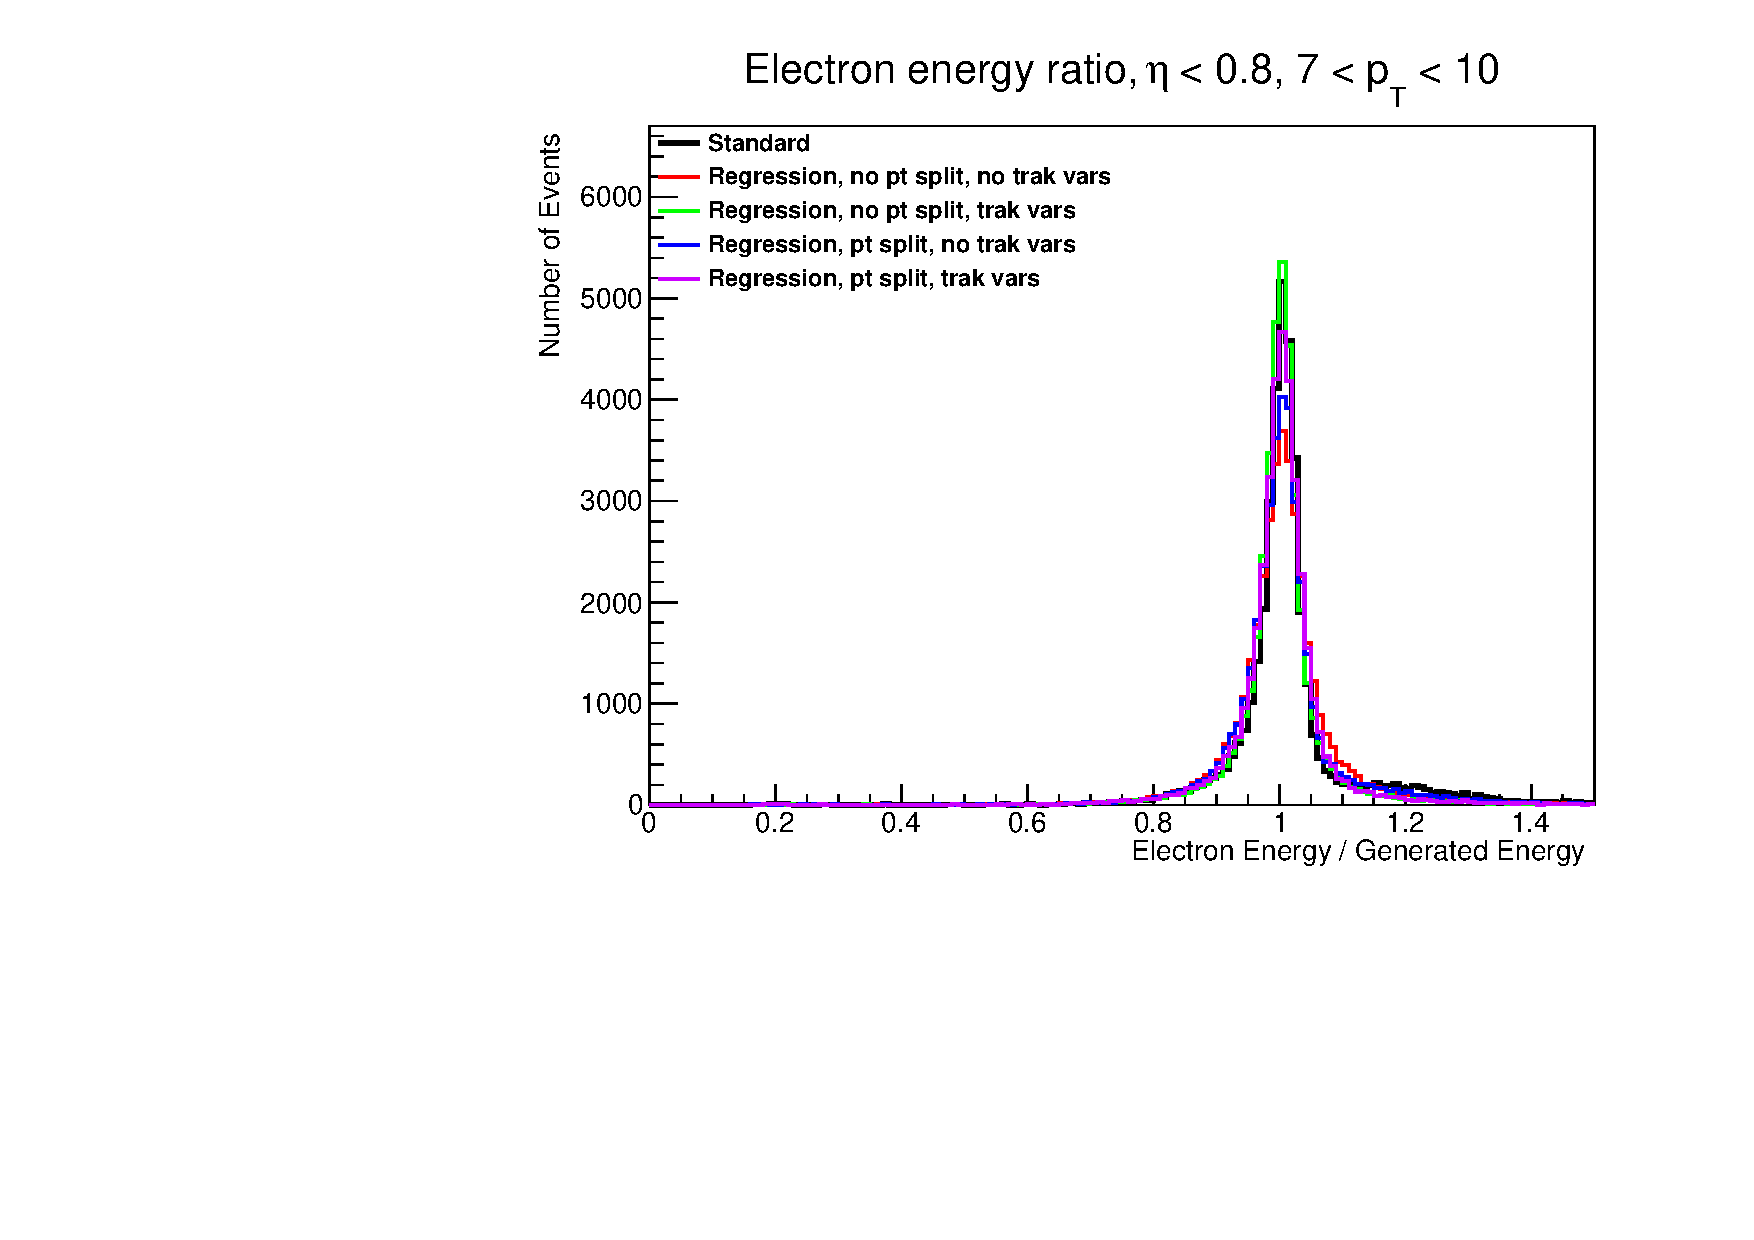
\includegraphics[width=0.6\textwidth]{figures/HZZ4l/EnergyResponse_allversions_binOption0.pdf}
		} \\
		\subfigure[]{
			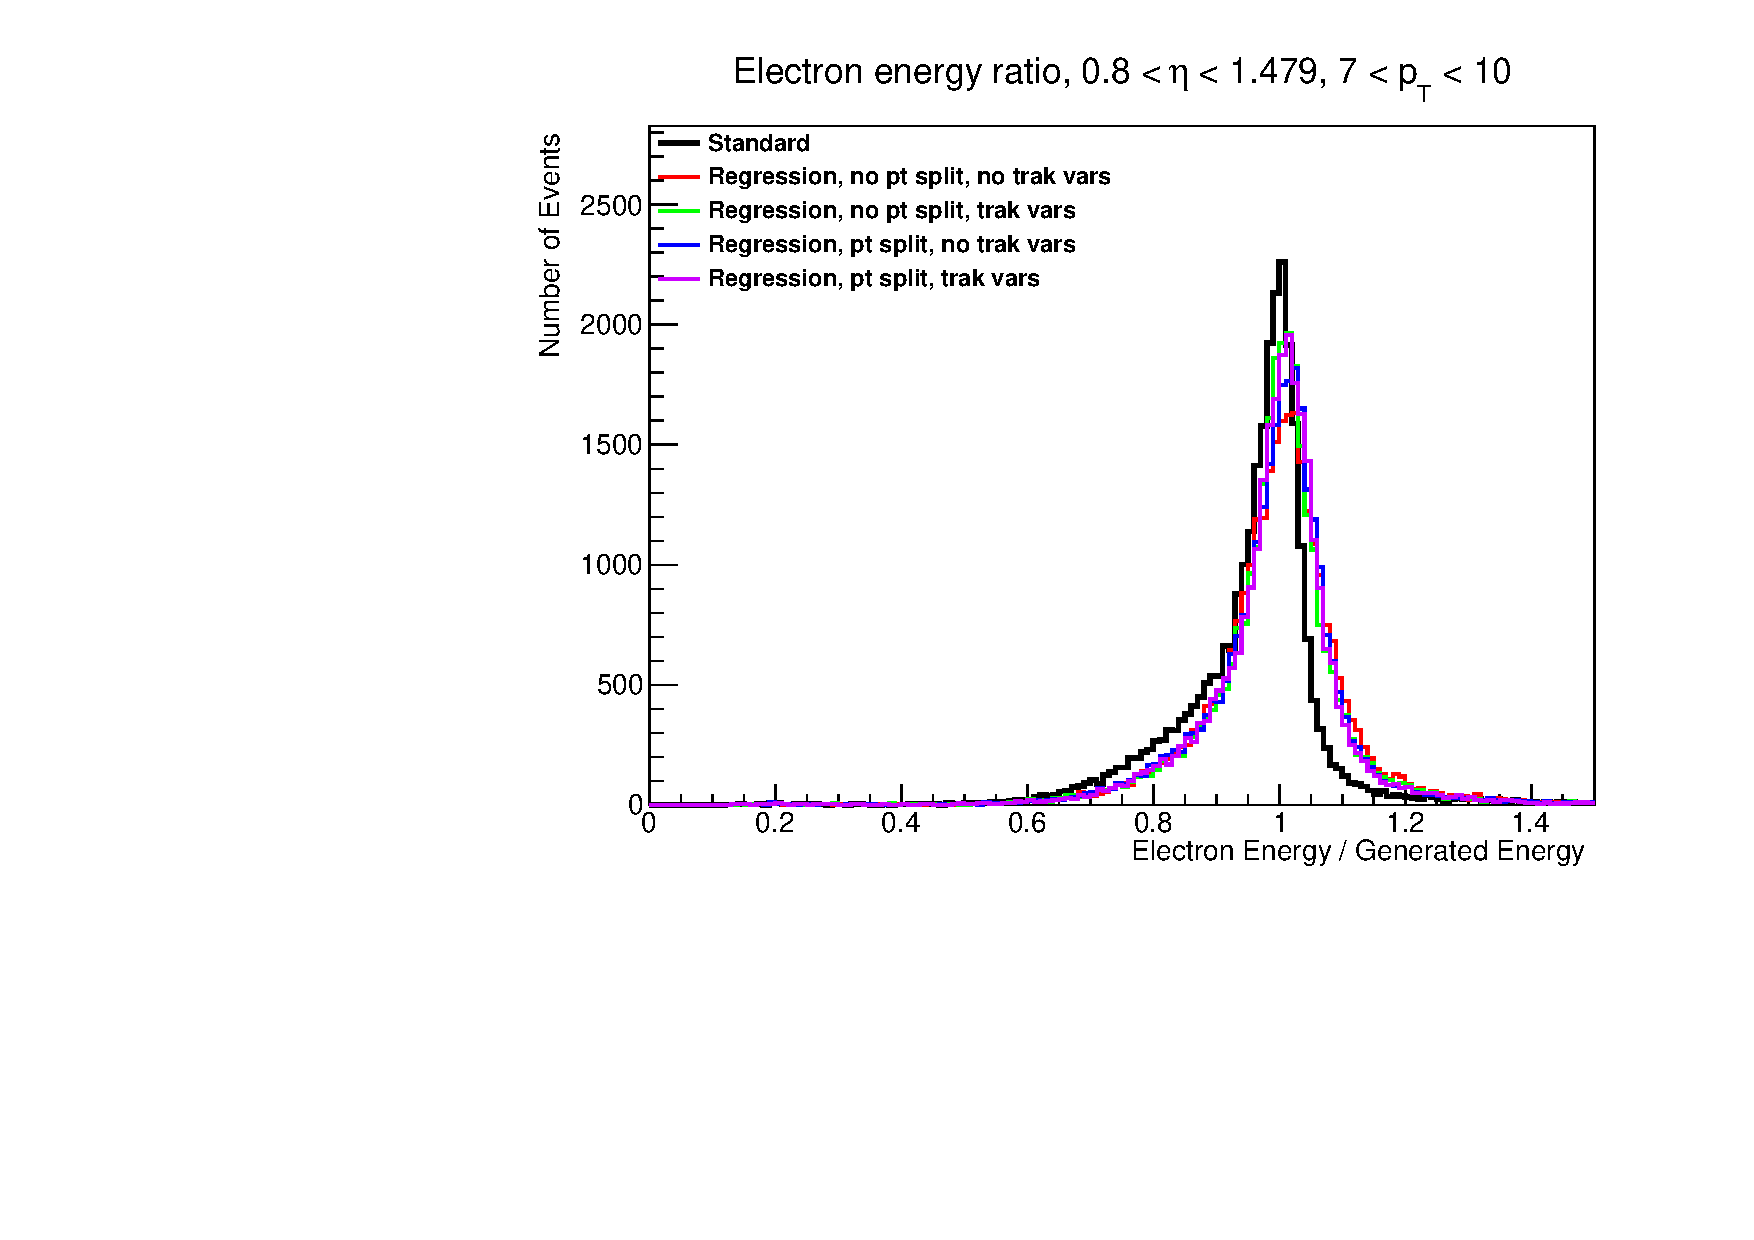
\includegraphics[width=0.6\textwidth]{figures/HZZ4l/EnergyResponse_allversions_binOption1.pdf}
		} \\
		\subfigure[]{
			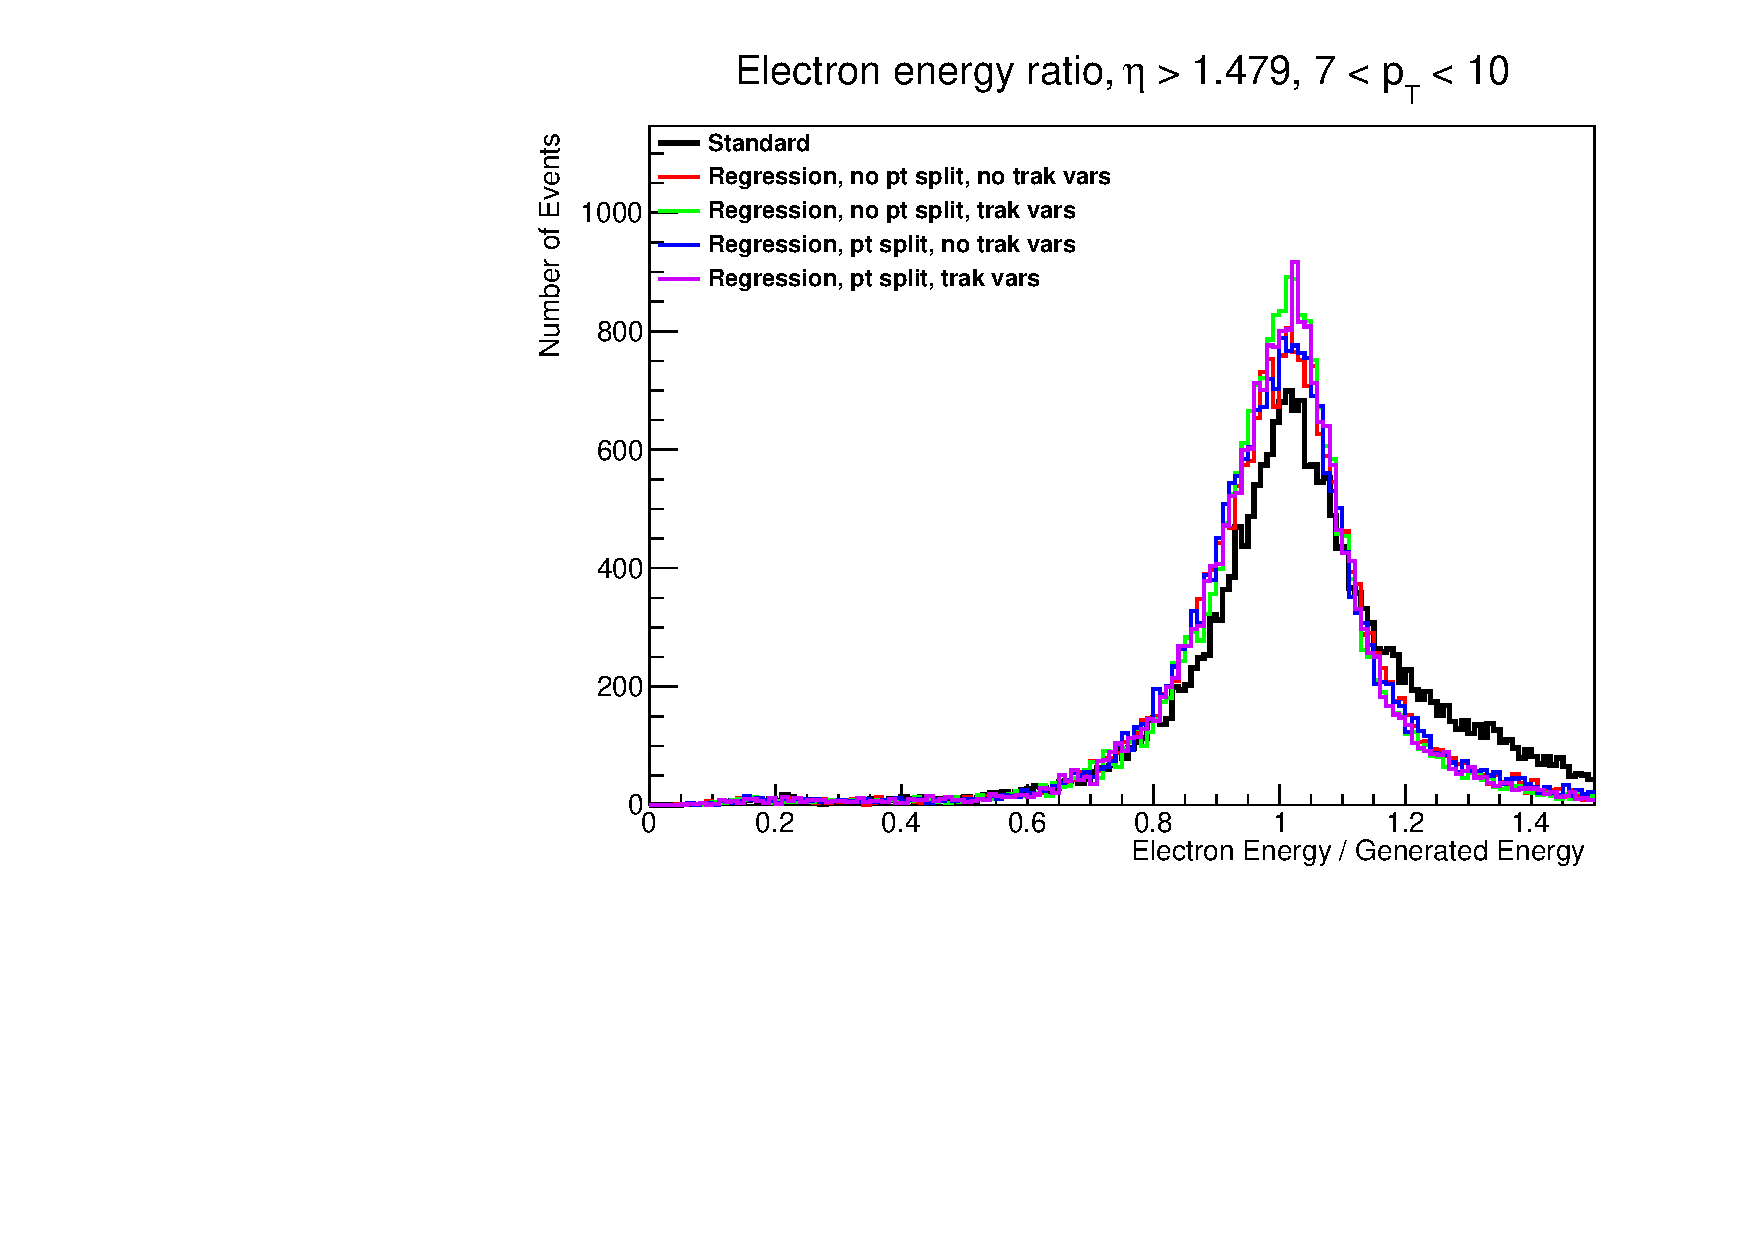
\includegraphics[width=0.6\textwidth]{figures/HZZ4l/EnergyResponse_allversions_binOption2.pdf}
		}
		\caption{Performance on Higgs Signal sample, low $p_T$ bins}
		\label{fig:higgssignalEnergyResponse1}
\end{figure}

\begin{figure}[h]
\centering
		\subfigure[]{
			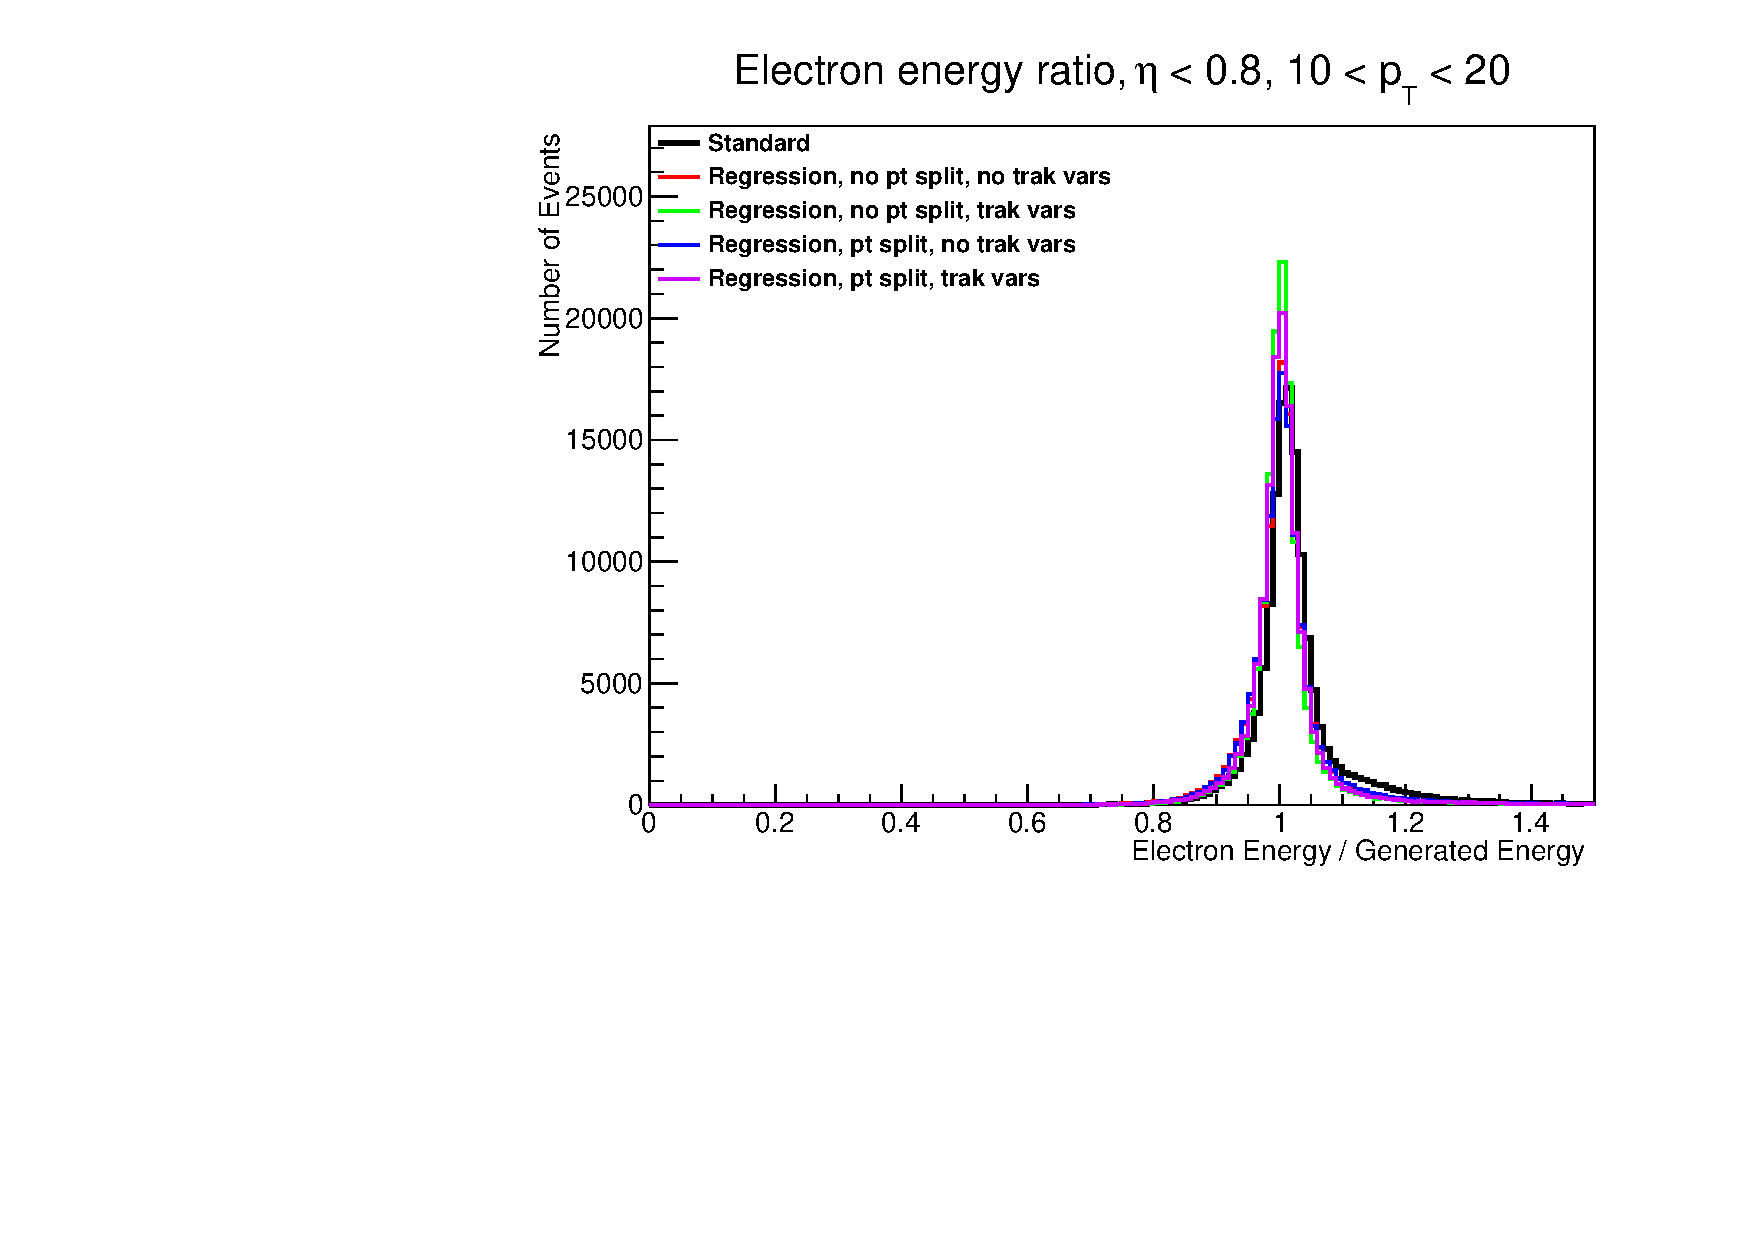
\includegraphics[width=0.6\textwidth]{figures/HZZ4l/EnergyResponse_allversions_binOption3.pdf}
		} \\
		\subfigure[]{
			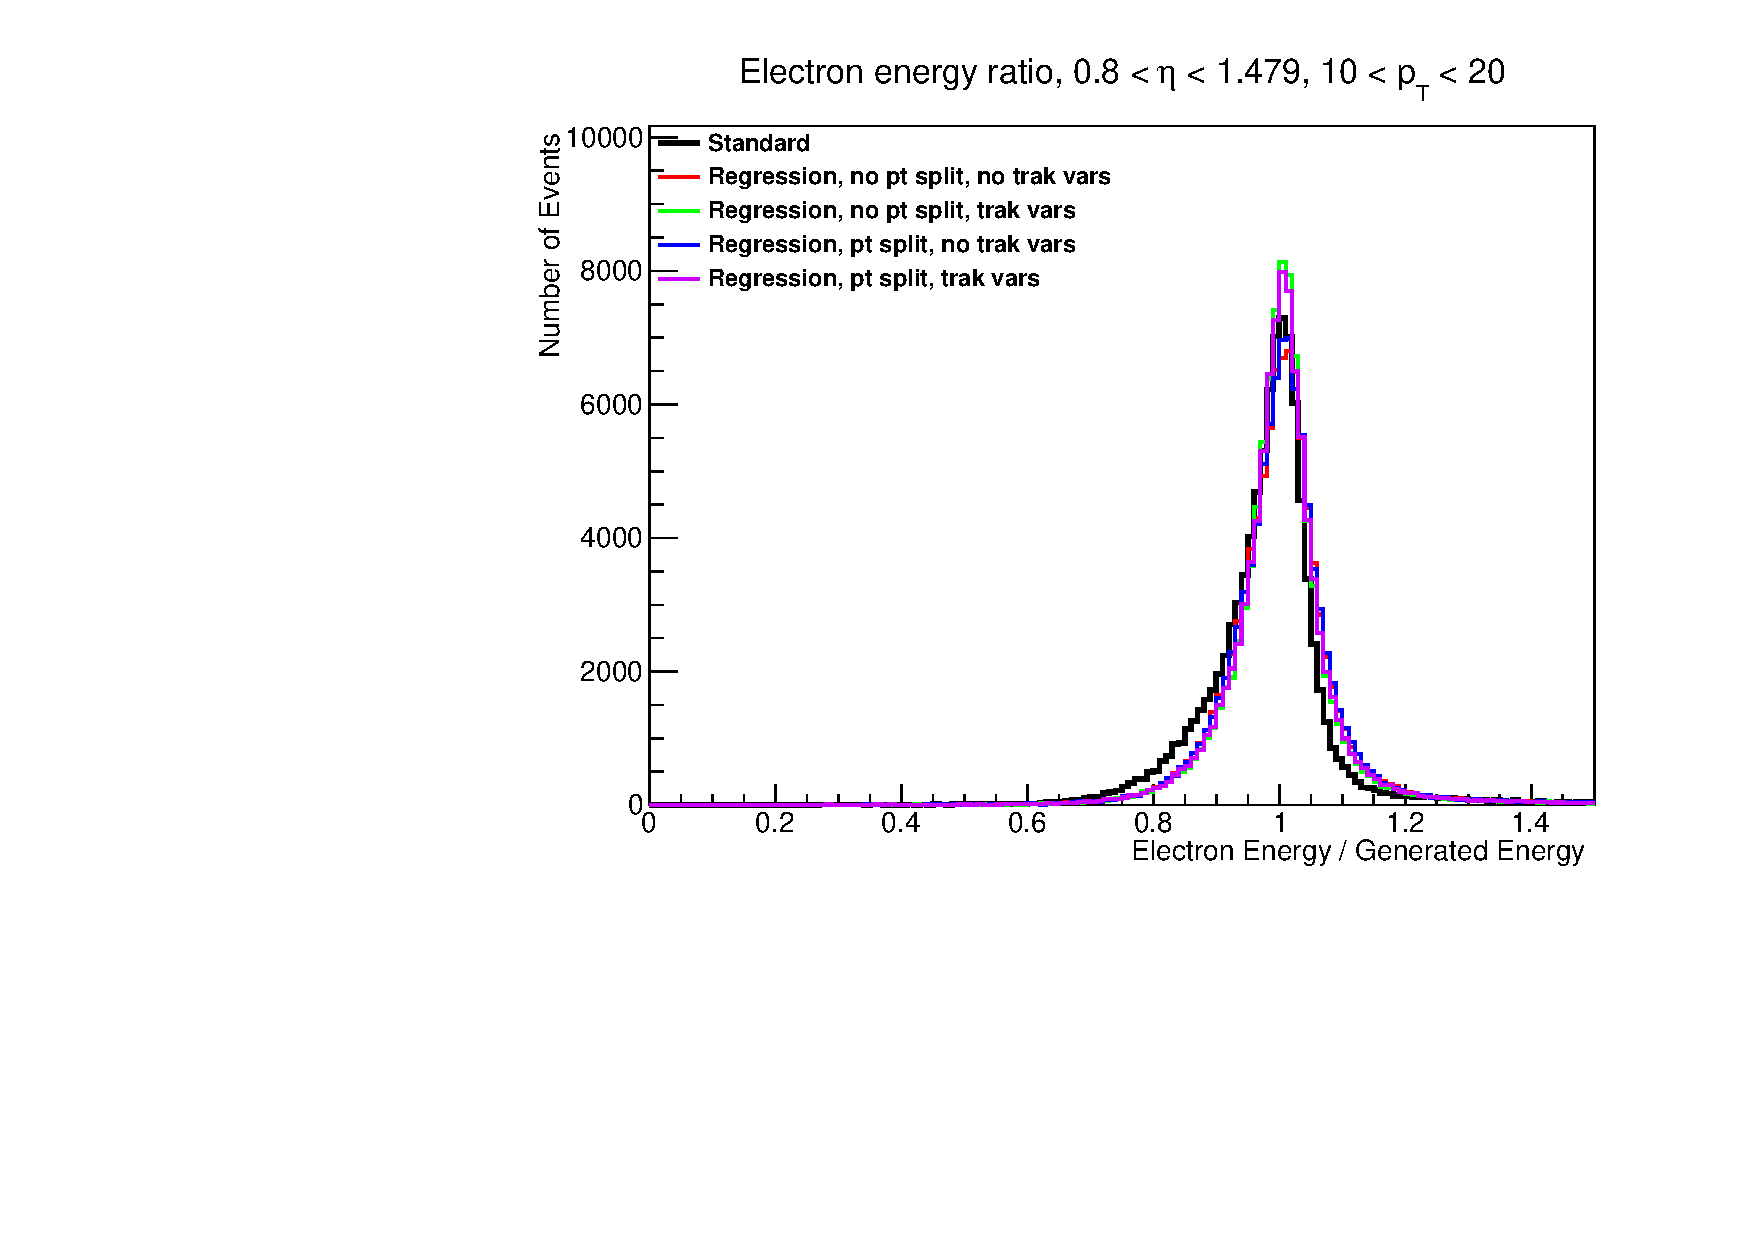
\includegraphics[width=0.6\textwidth]{figures/HZZ4l/EnergyResponse_allversions_binOption4.pdf}
		} \\
		\subfigure[]{
			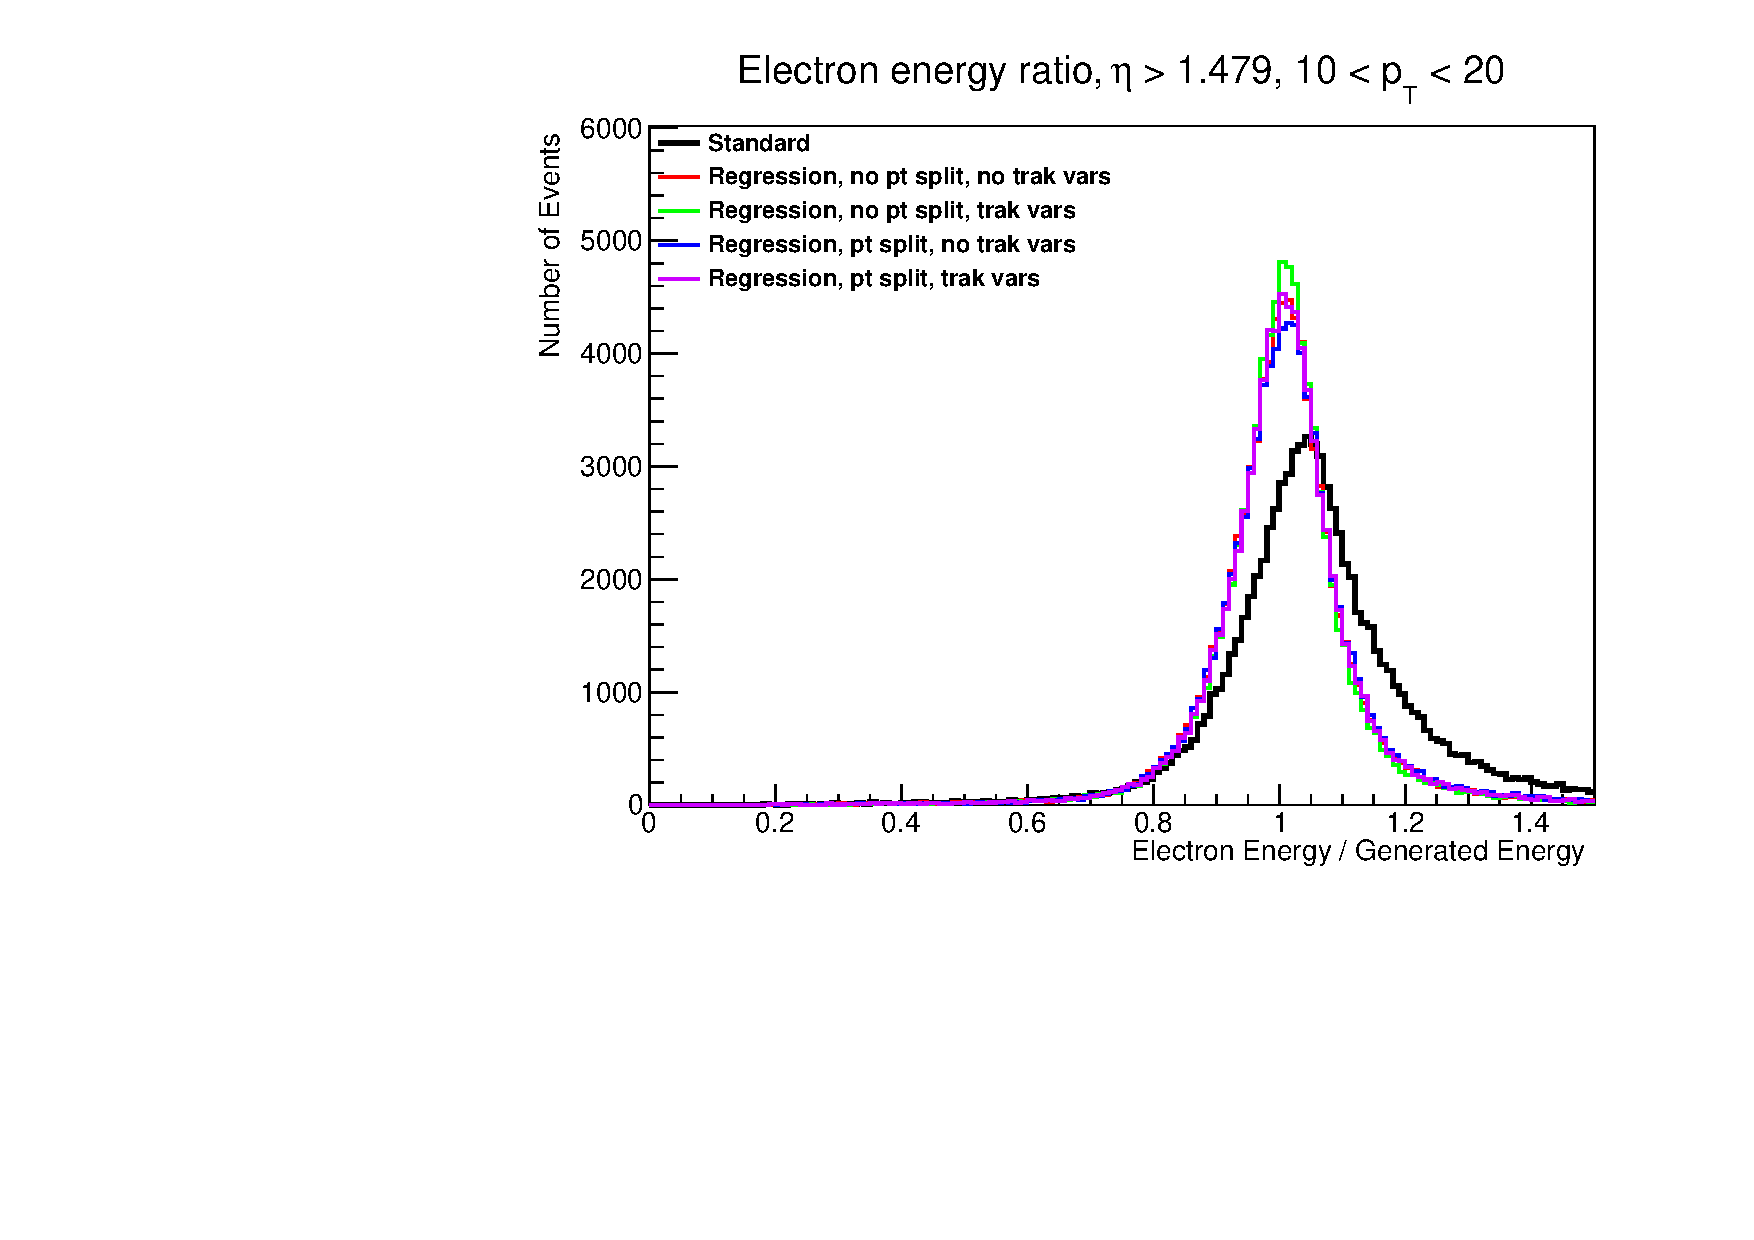
\includegraphics[width=0.6\textwidth]{figures/HZZ4l/EnergyResponse_allversions_binOption5.pdf}
		}
		\caption{Performance on Higgs Signal sample, medium $p_T$ bins}
		\label{fig:higgssignalEnergyResponse2}
\end{figure}

\begin{figure}[h]
\centering
		\subfigure[]{
			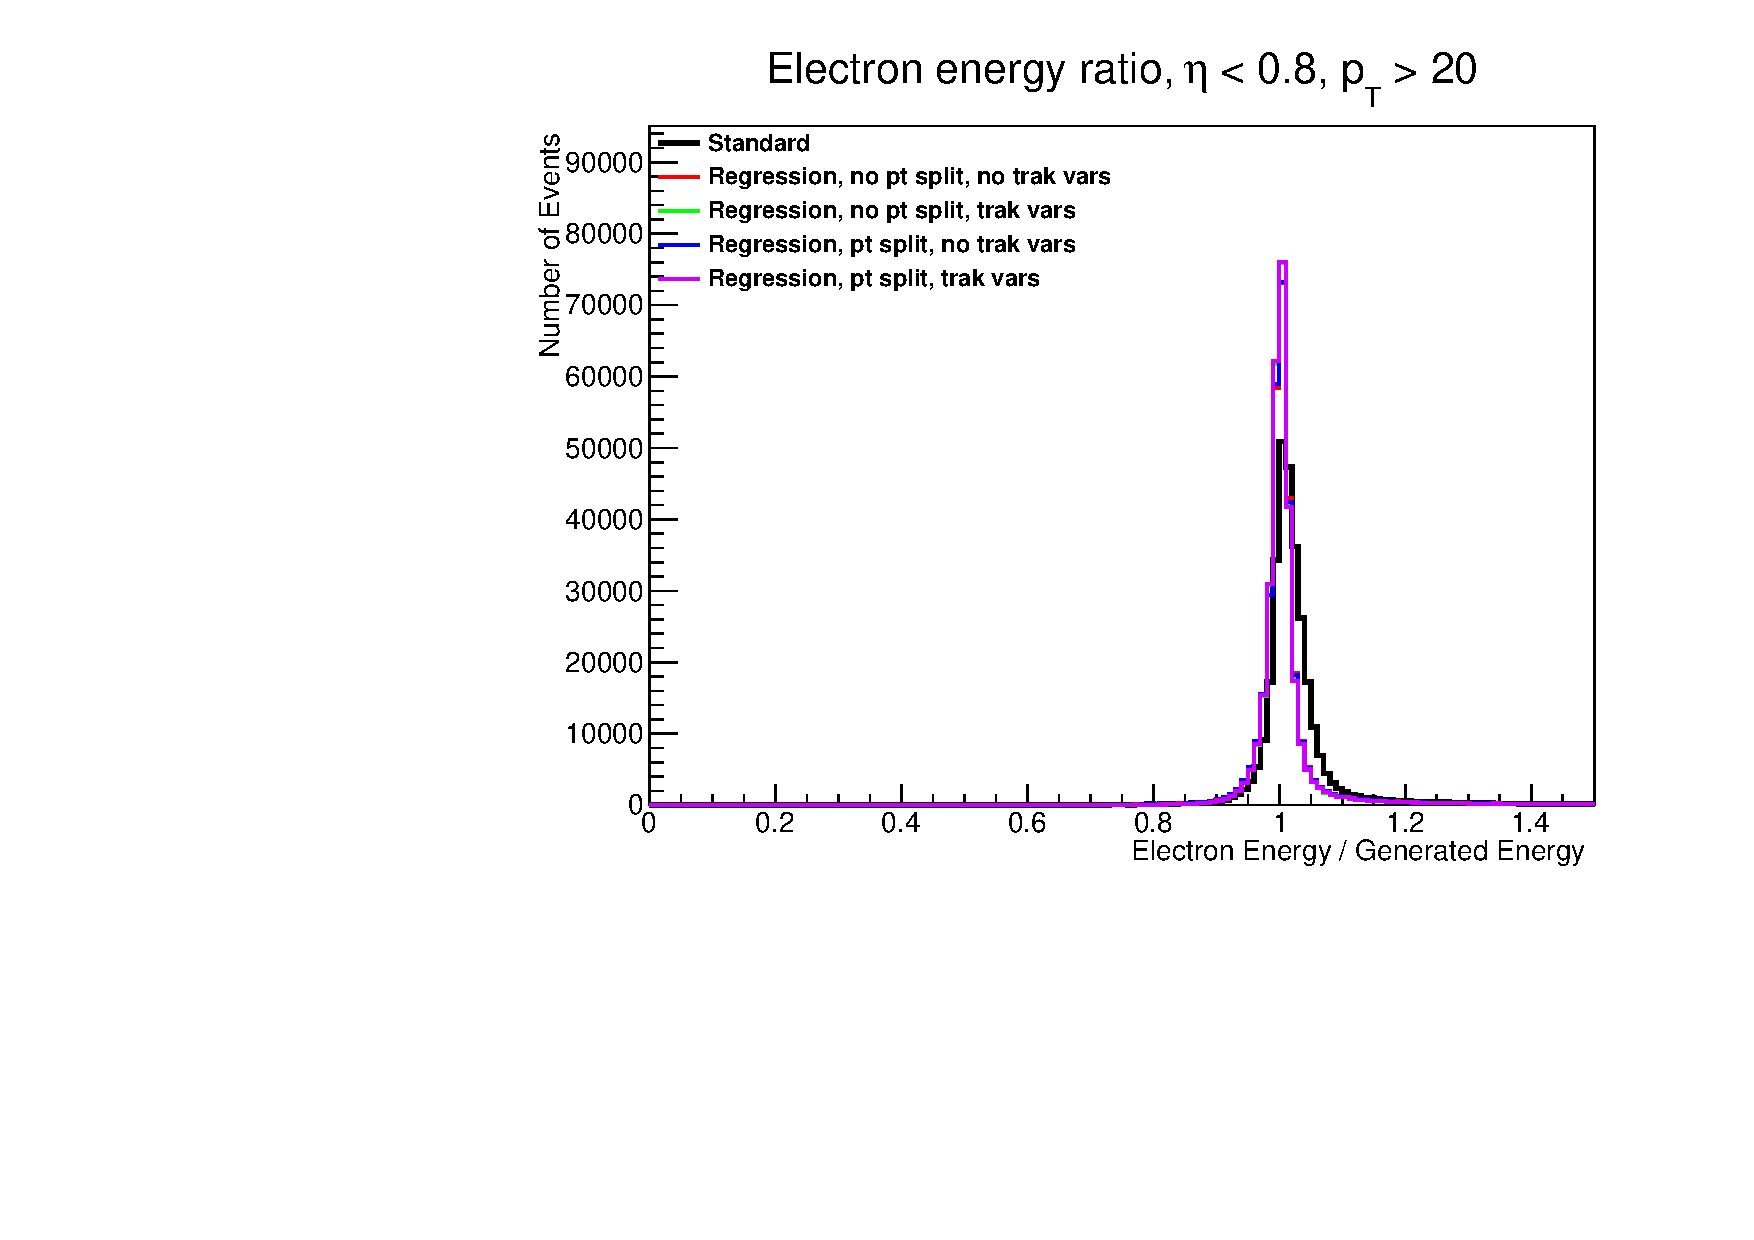
\includegraphics[width=0.6\textwidth]{figures/HZZ4l/EnergyResponse_allversions_binOption6.pdf}
		} \\
		\subfigure[]{
			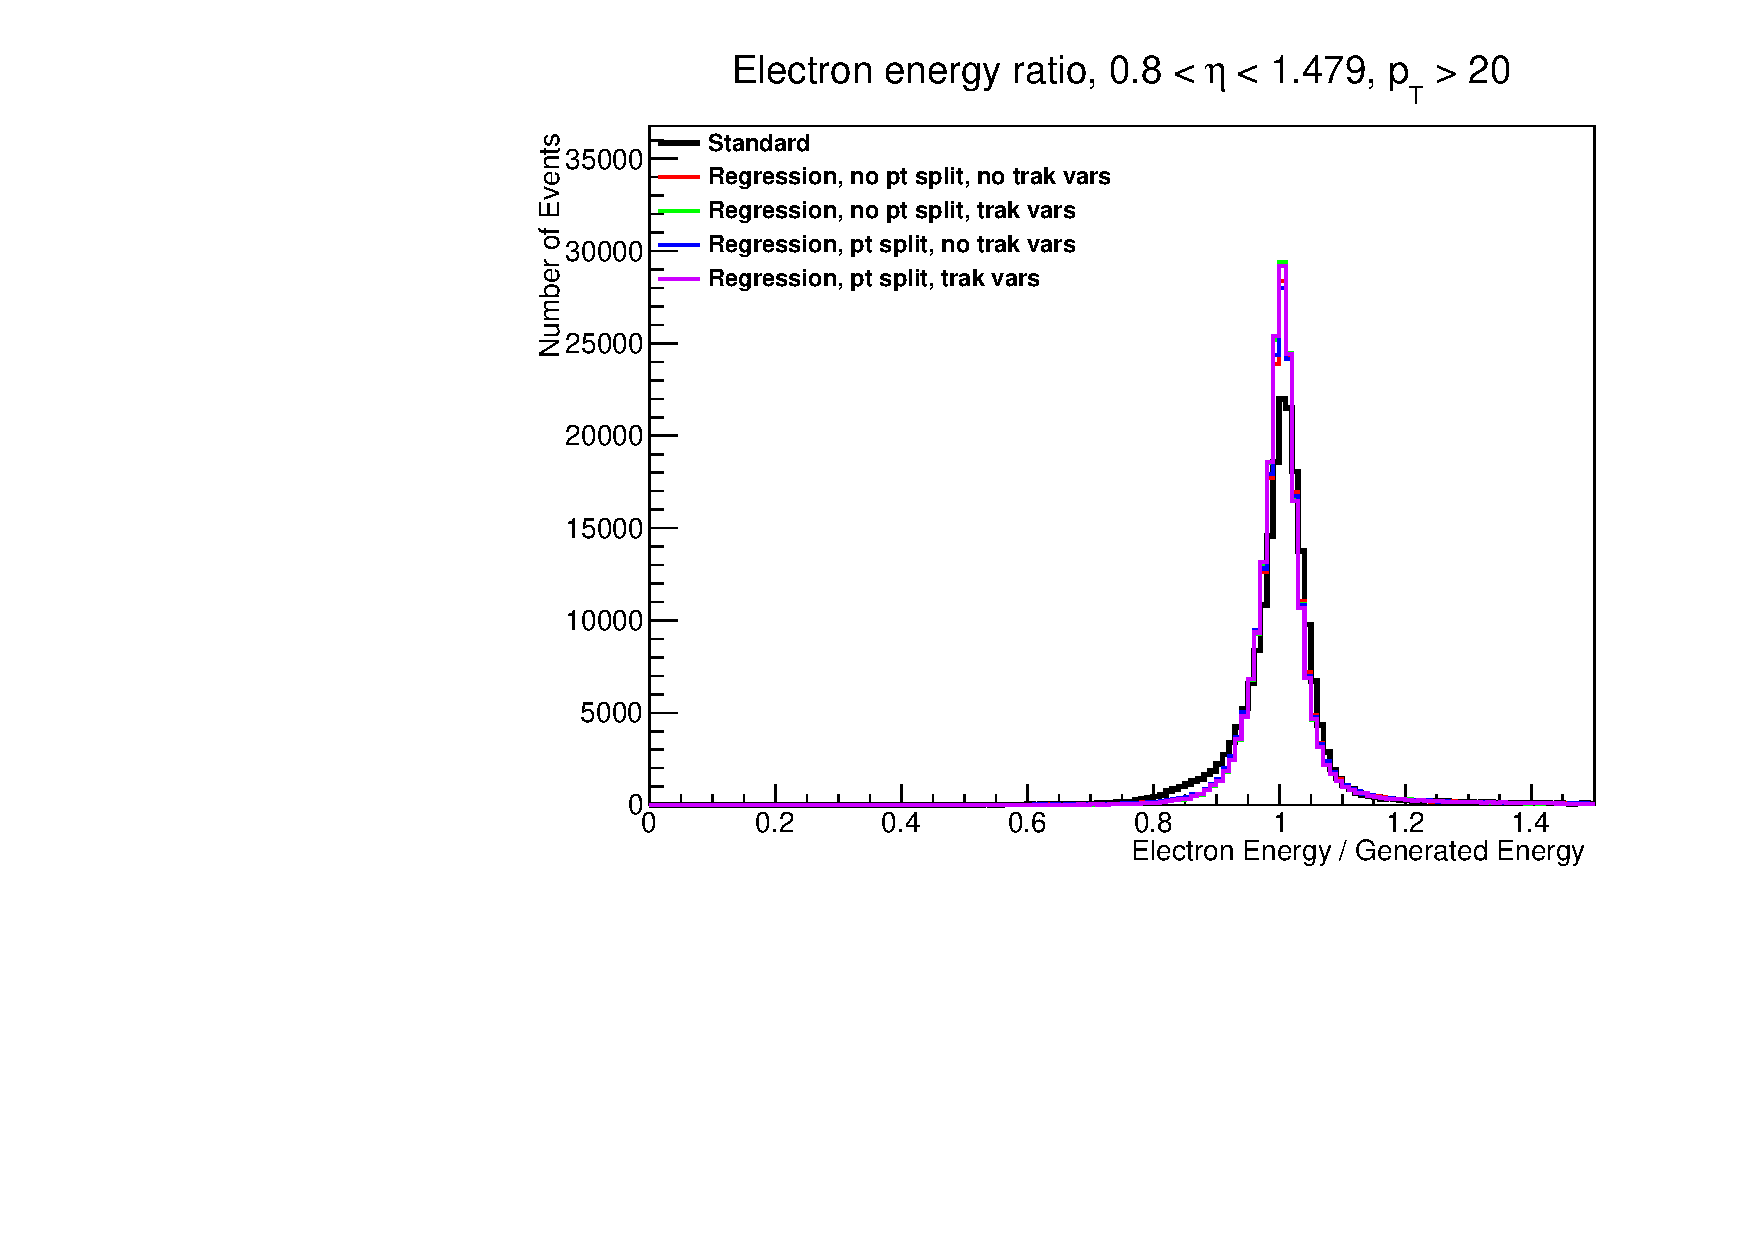
\includegraphics[width=0.6\textwidth]{figures/HZZ4l/EnergyResponse_allversions_binOption7.pdf}
		} \\
		\subfigure[]{
			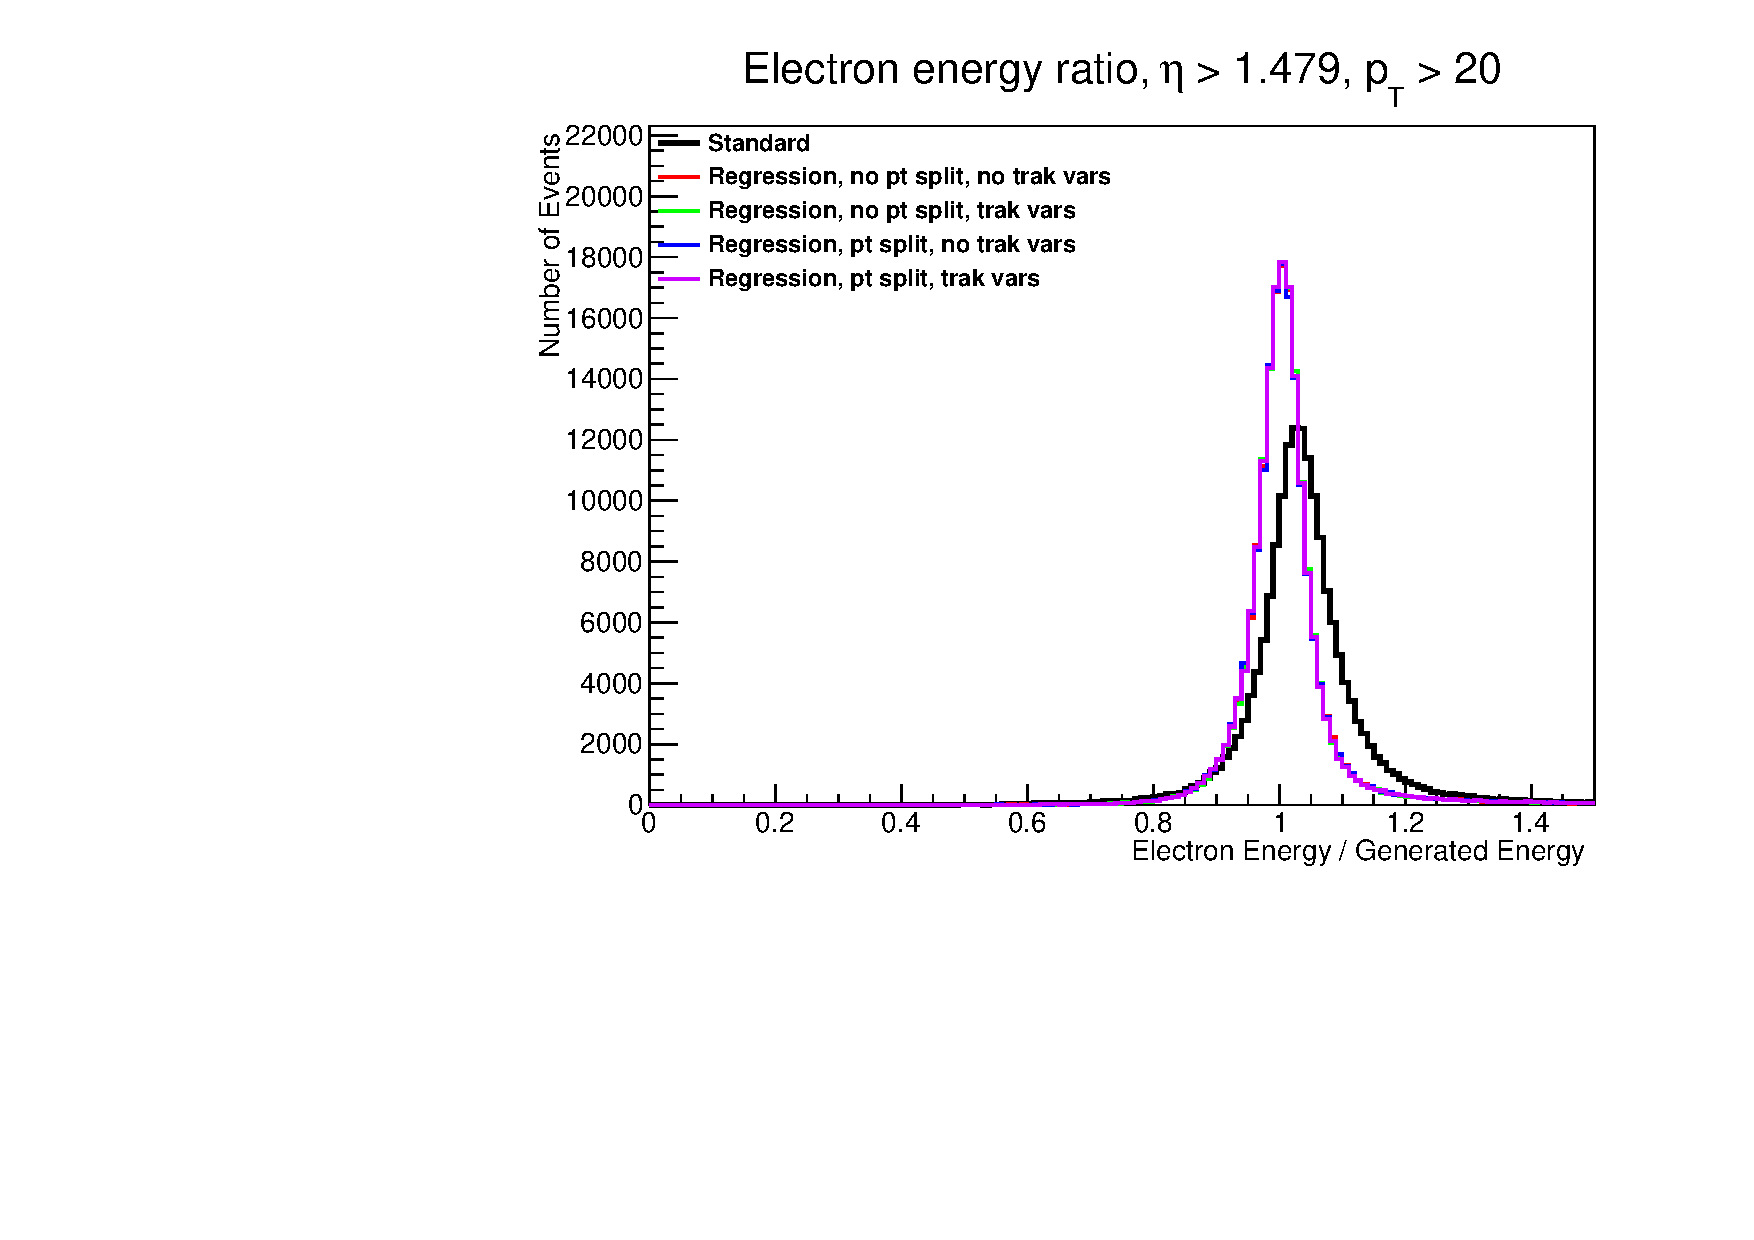
\includegraphics[width=0.6\textwidth]{figures/HZZ4l/EnergyResponse_allversions_binOption8.pdf}
		}
		\caption{Performance on Higgs Signal sample, high $p_T$ bins}
		\label{fig:higgssignalEnergyResponse3}
\end{figure}

%% Figures for Drell-Yan
\begin{figure}[h]
\centering
		\subfigure[]{
			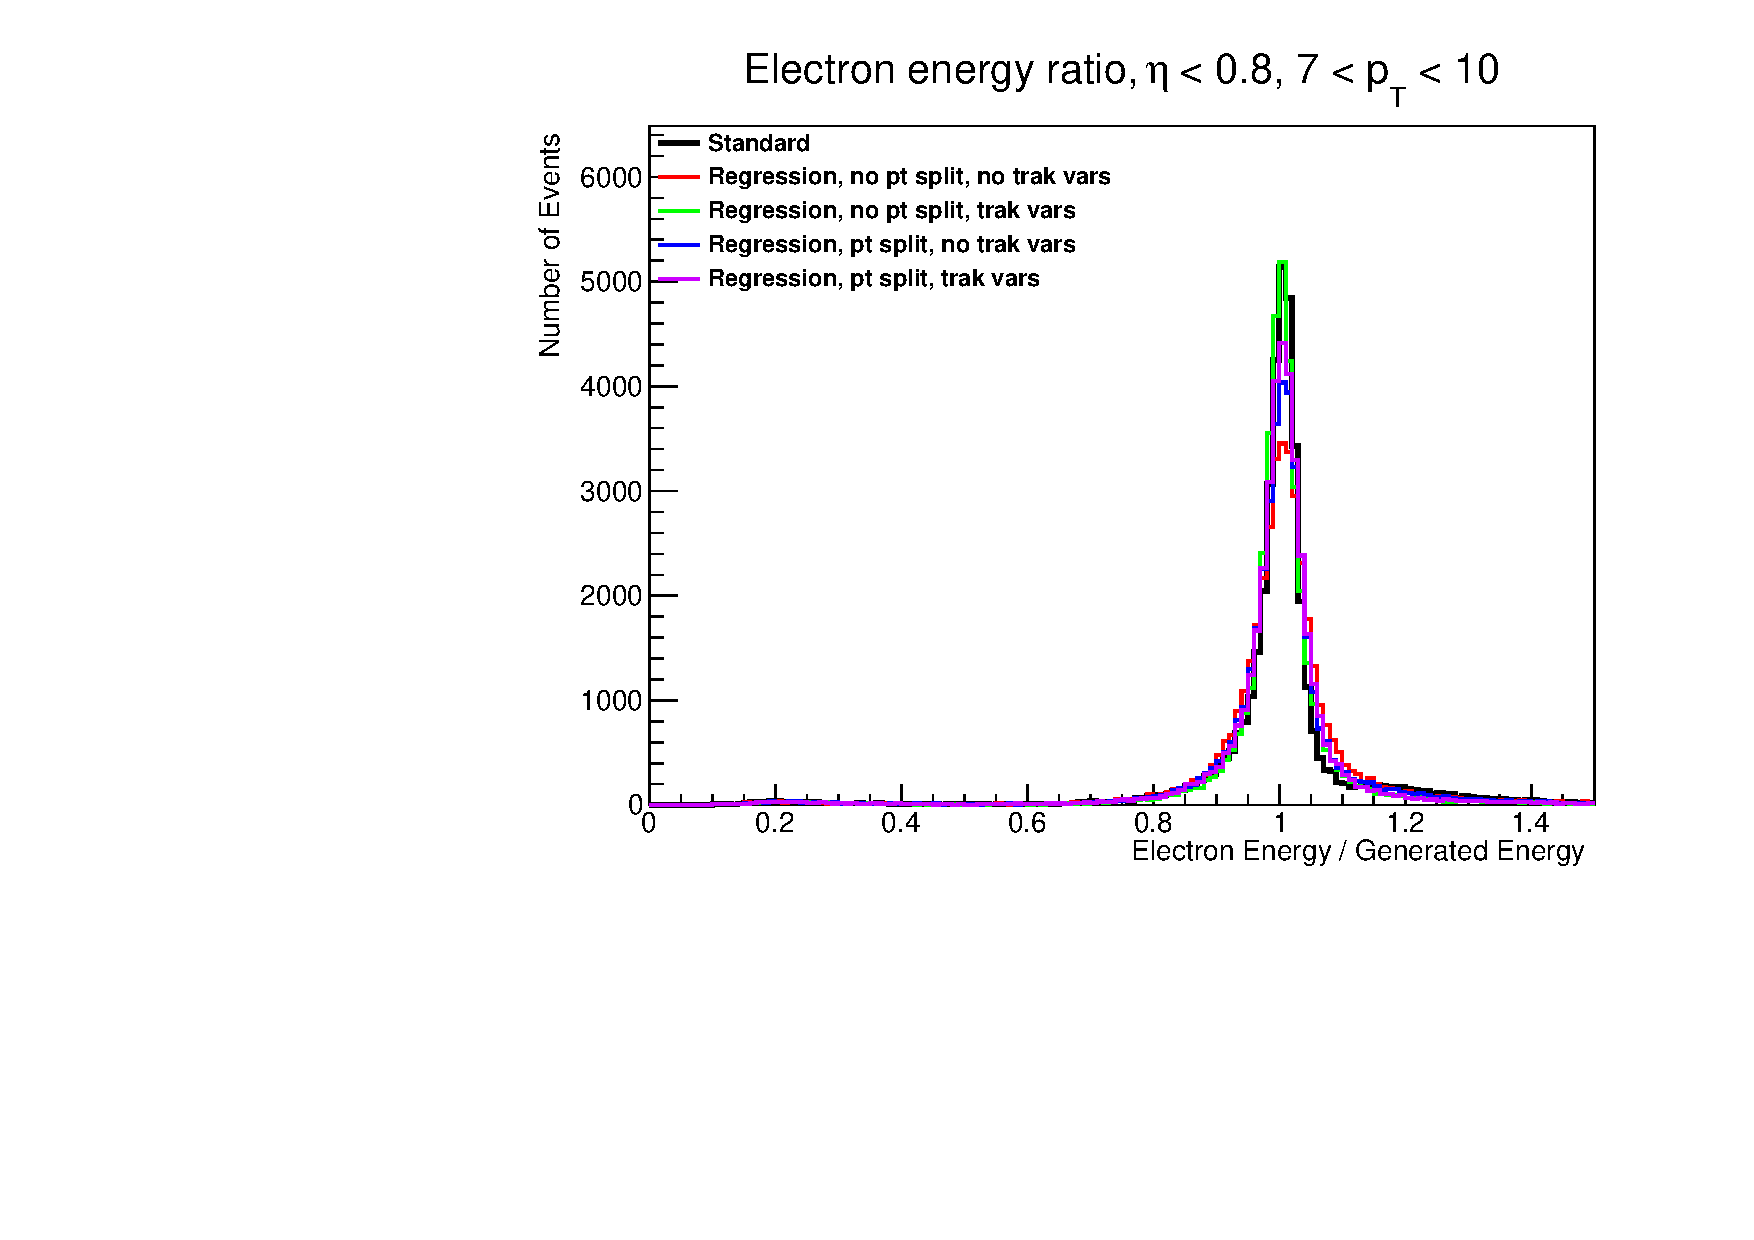
\includegraphics[width=0.6\textwidth]{figures/DY/EnergyResponse_allversions_binOption0.pdf}
		} \\
		\subfigure[]{
			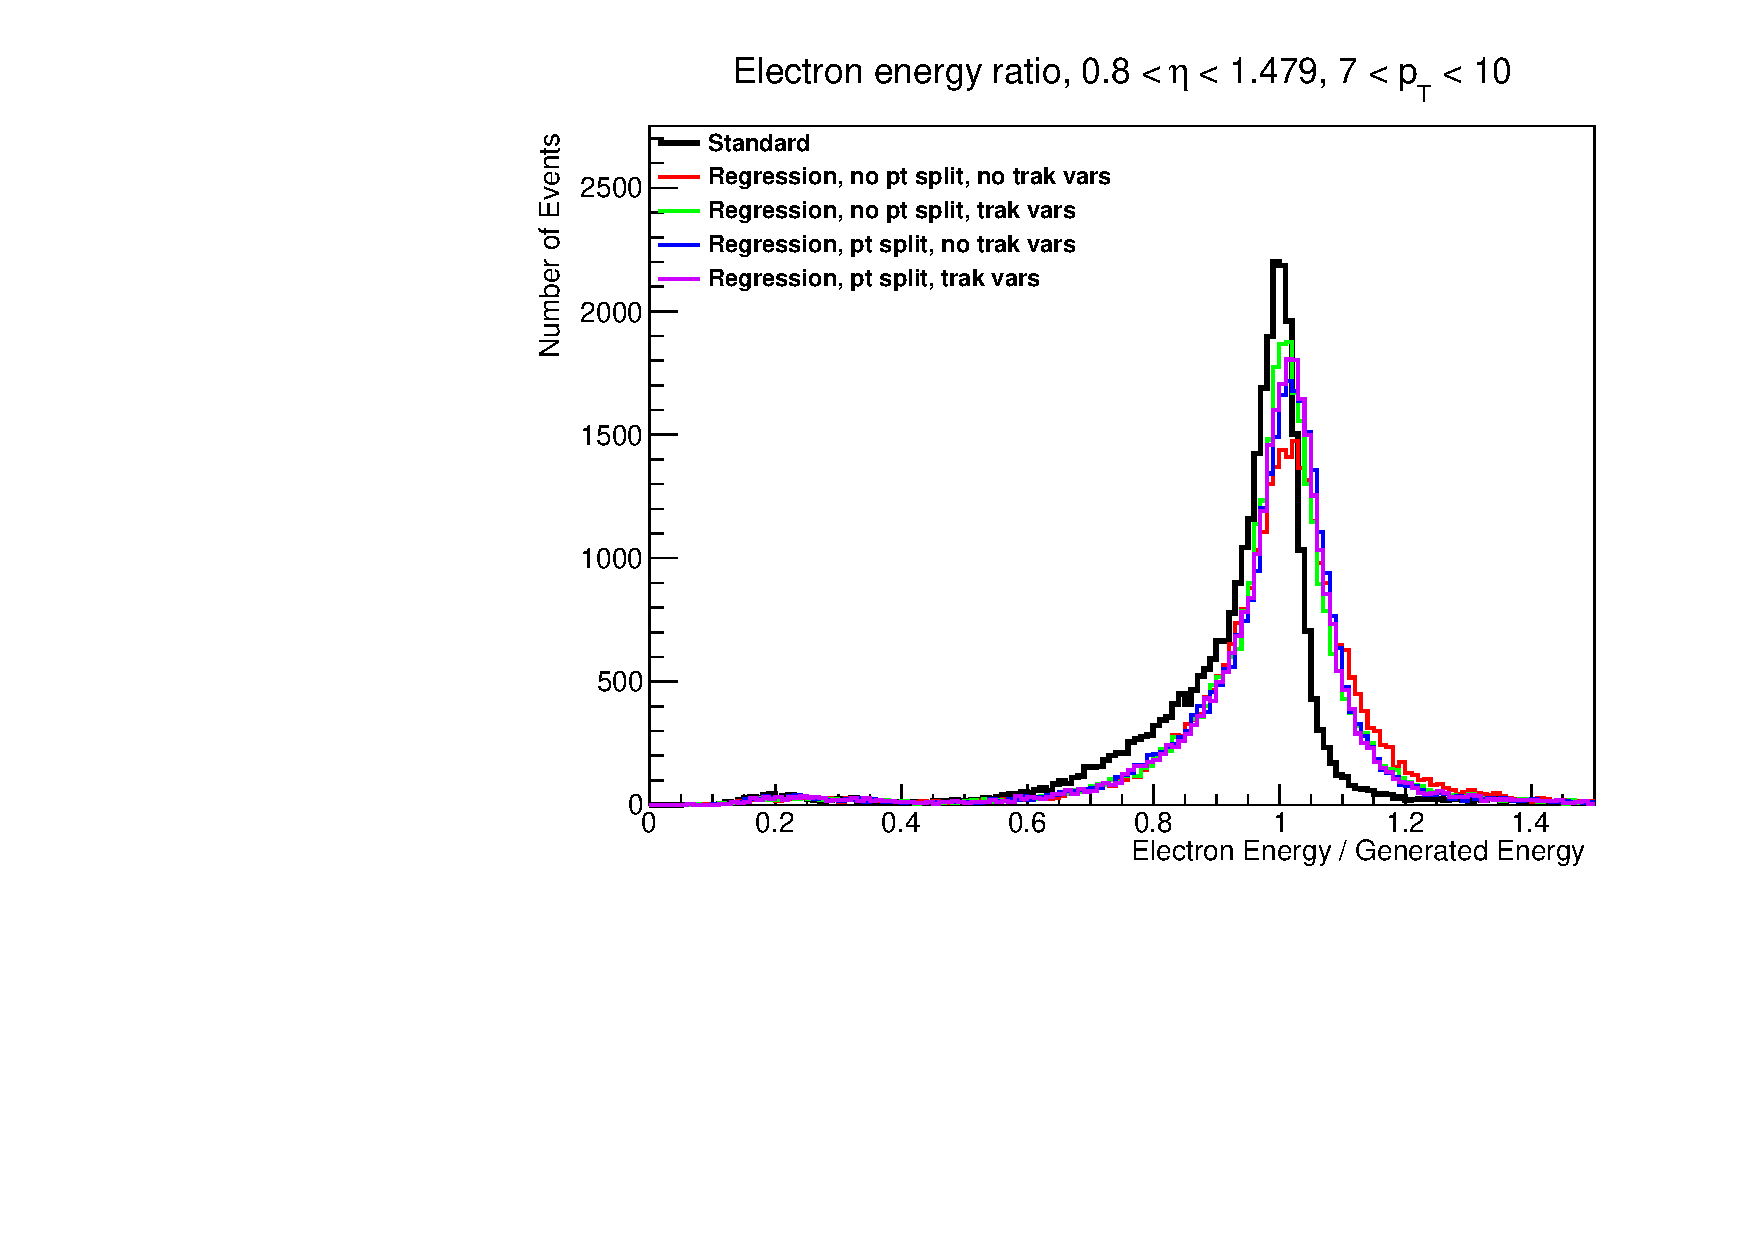
\includegraphics[width=0.6\textwidth]{figures/DY/EnergyResponse_allversions_binOption1.pdf}
		} \\
		\subfigure[]{
			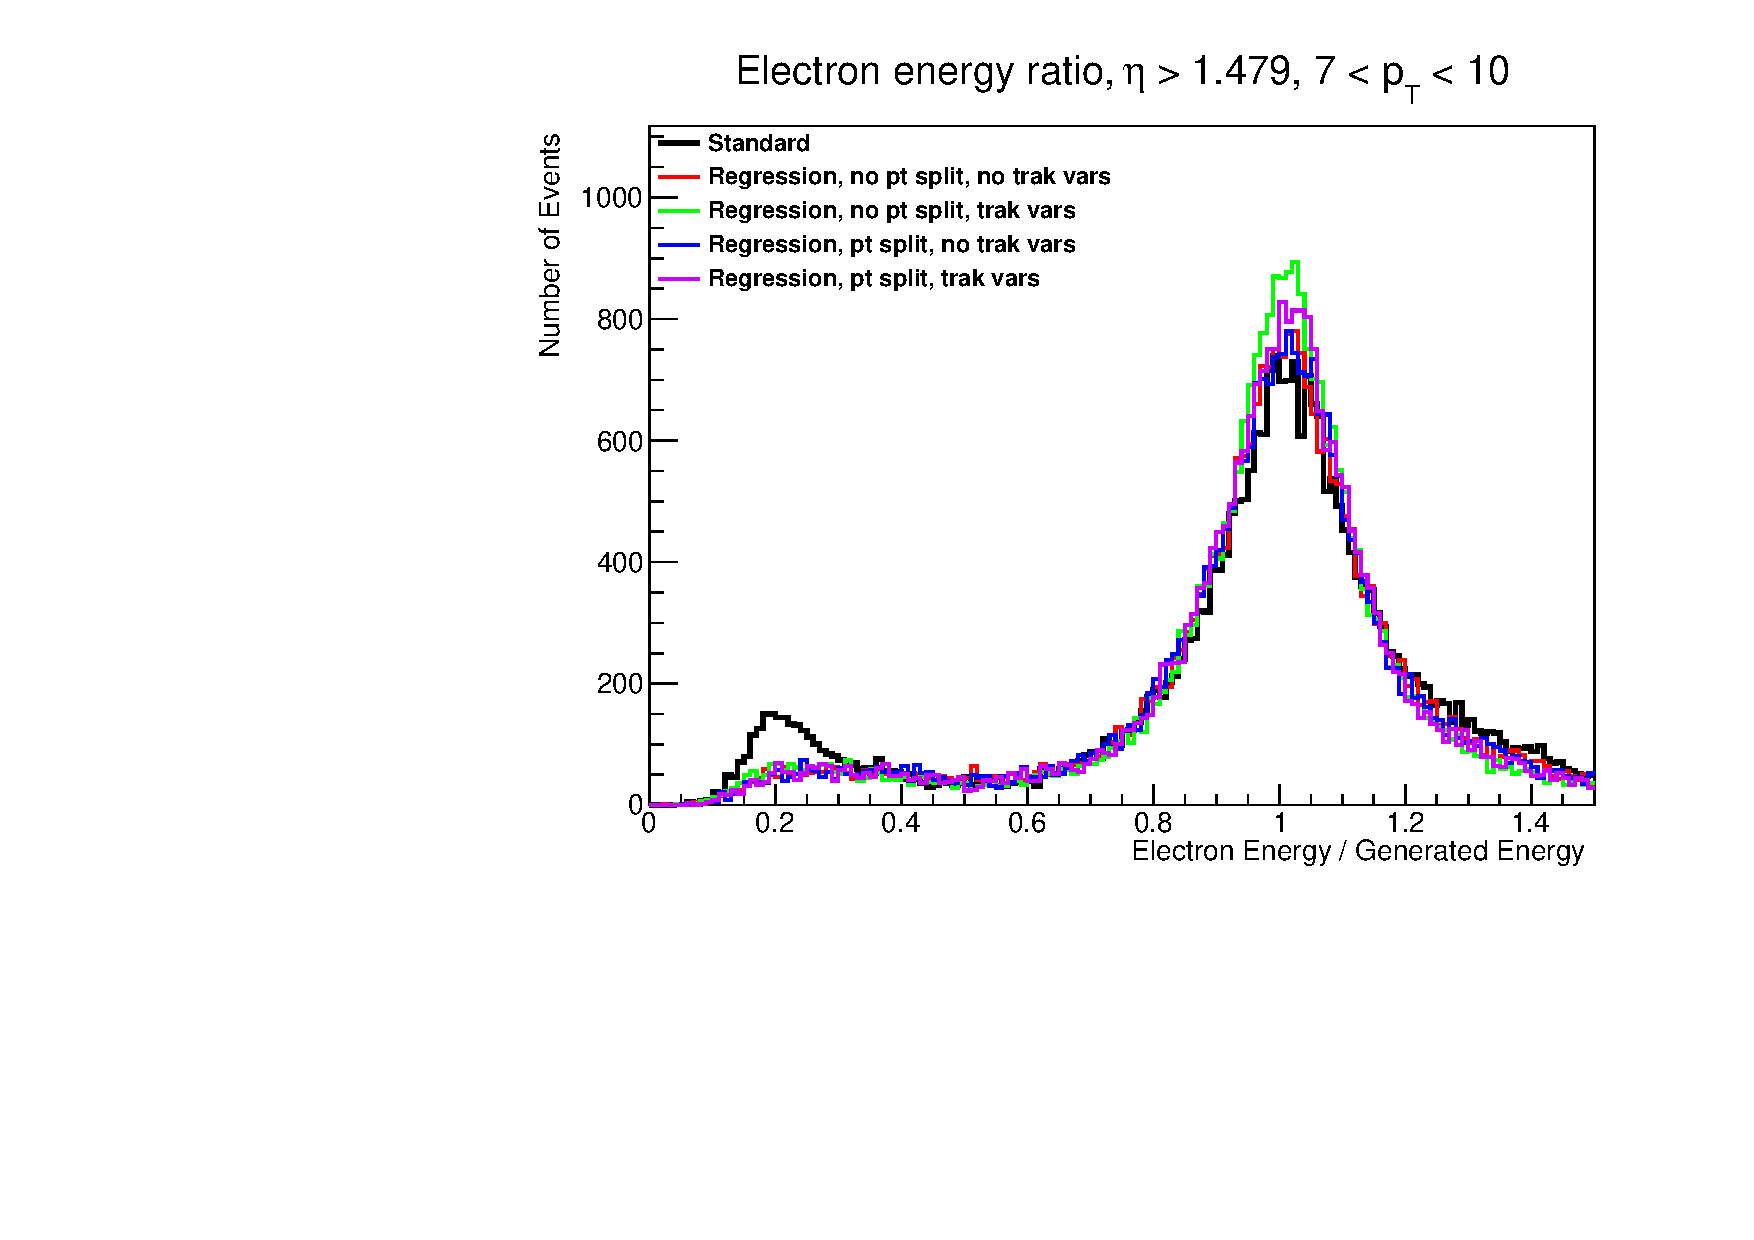
\includegraphics[width=0.6\textwidth]{figures/DY/EnergyResponse_allversions_binOption2.pdf}
		}
		\caption{Performance on Drell-Yan sample, low $p_T$ bins}
		\label{fig:drellyanEnergyResponse1}
\end{figure}

\begin{figure}[h]
\centering
		\subfigure[]{
			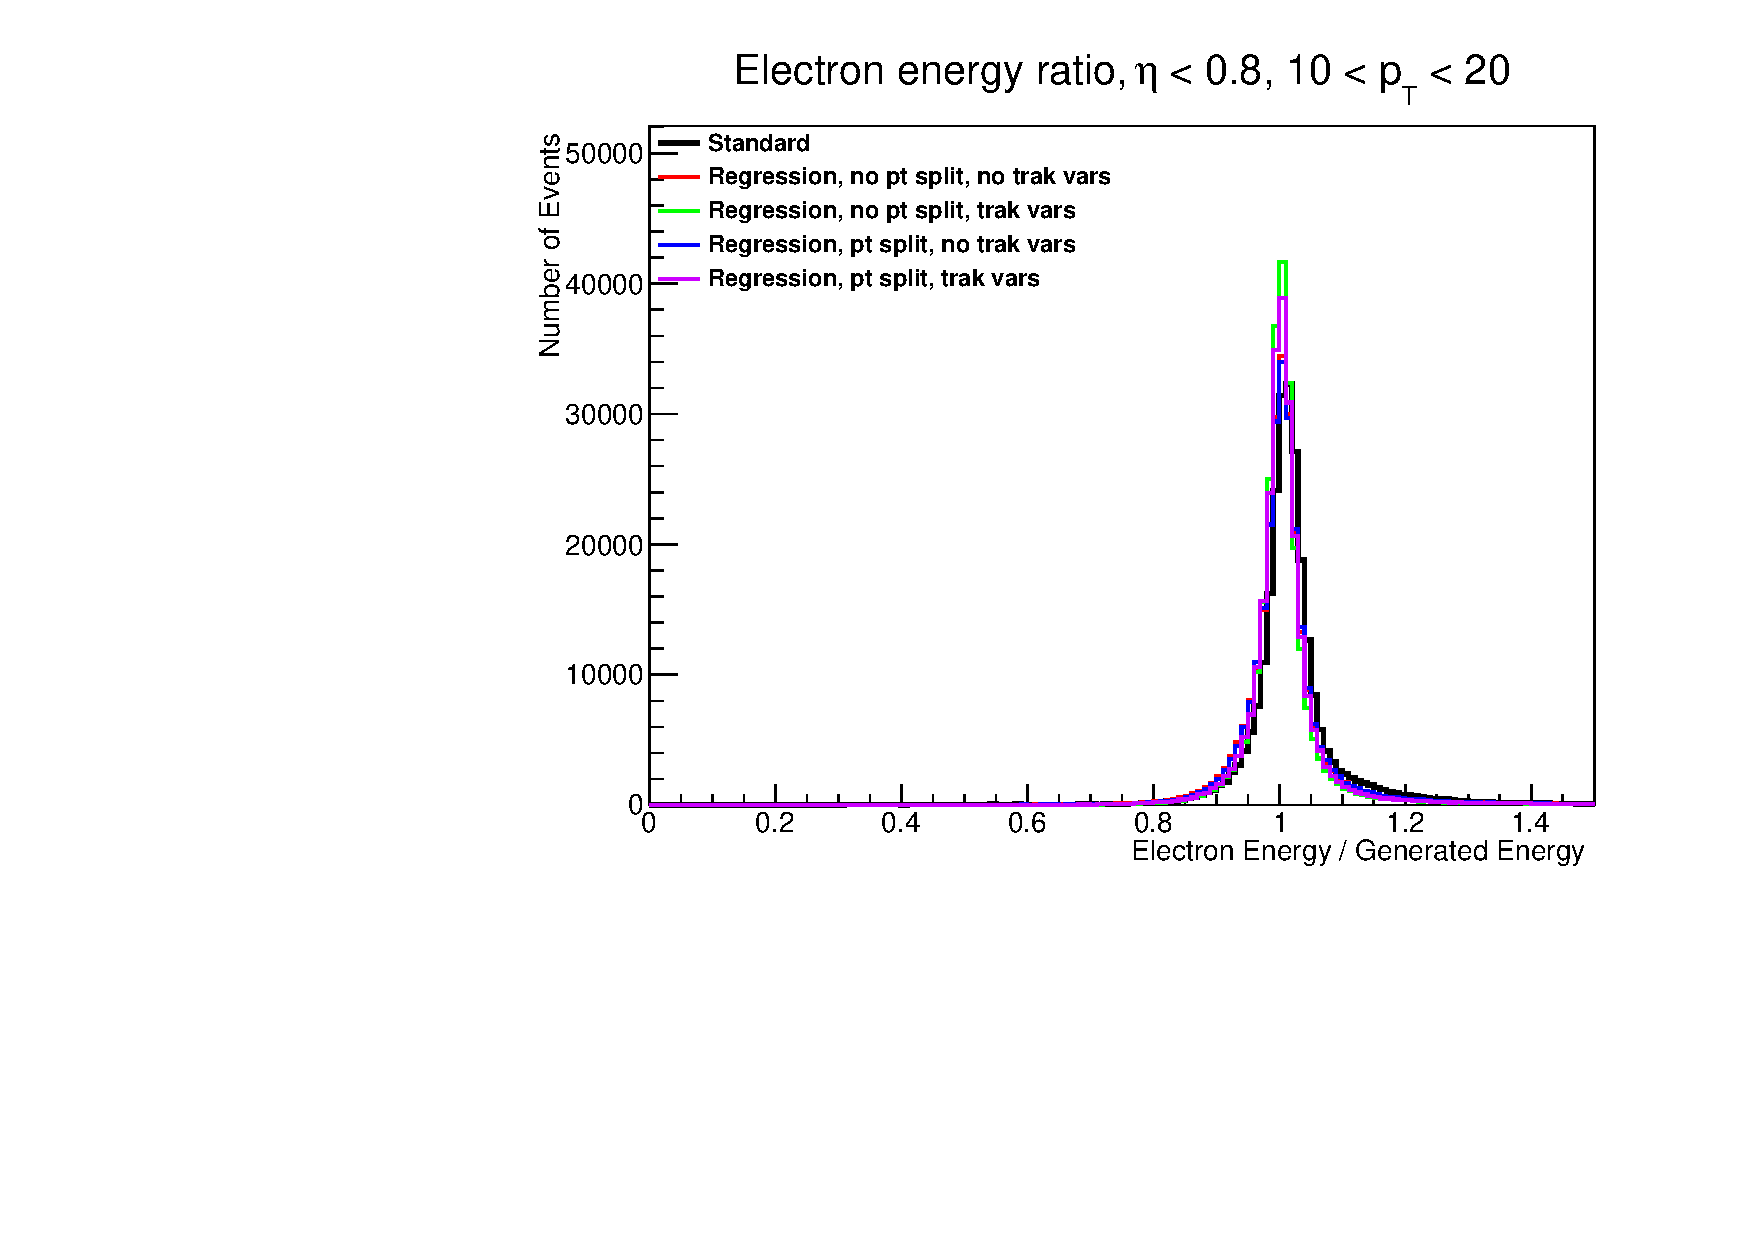
\includegraphics[width=0.6\textwidth]{figures/DY/EnergyResponse_allversions_binOption3.pdf}
		} \\
		\subfigure[]{
			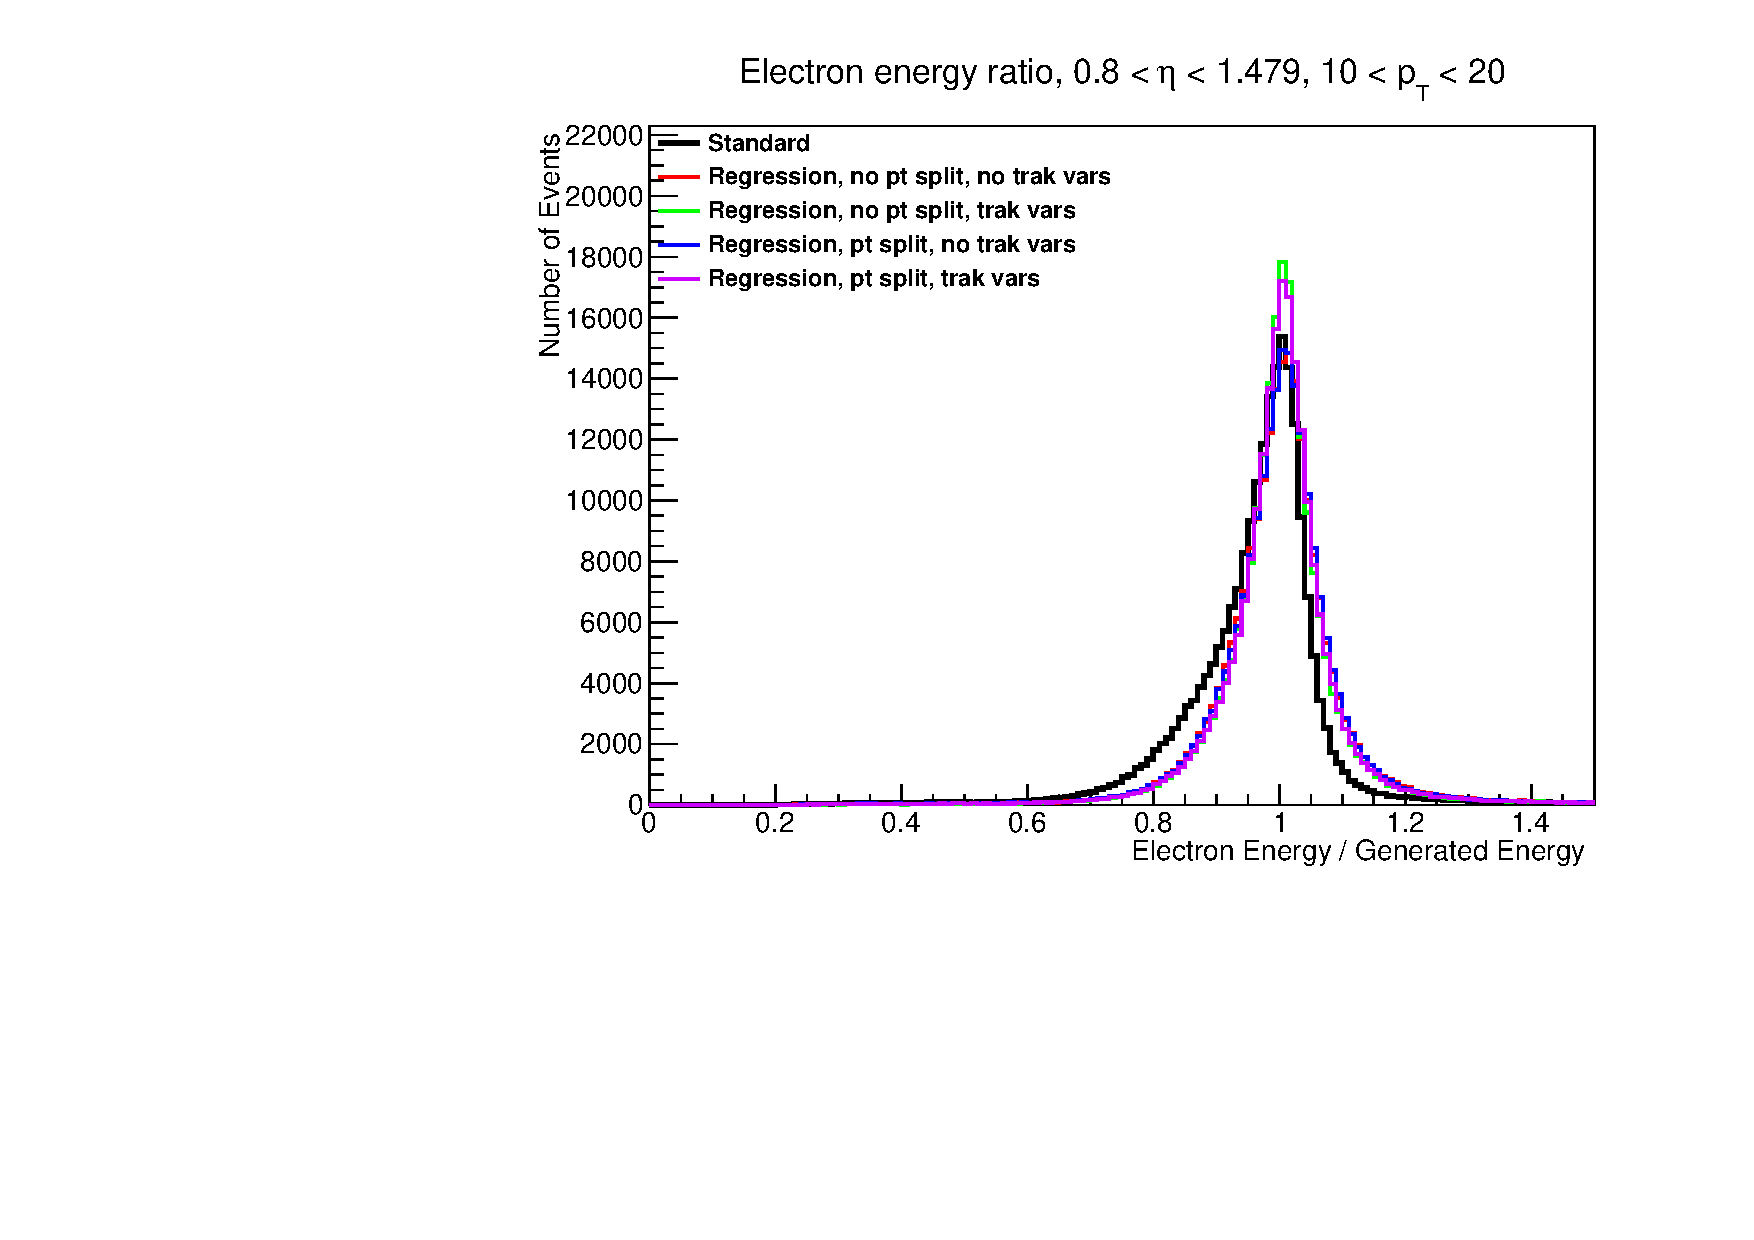
\includegraphics[width=0.6\textwidth]{figures/DY/EnergyResponse_allversions_binOption4.pdf}
		} \\
		\subfigure[]{
			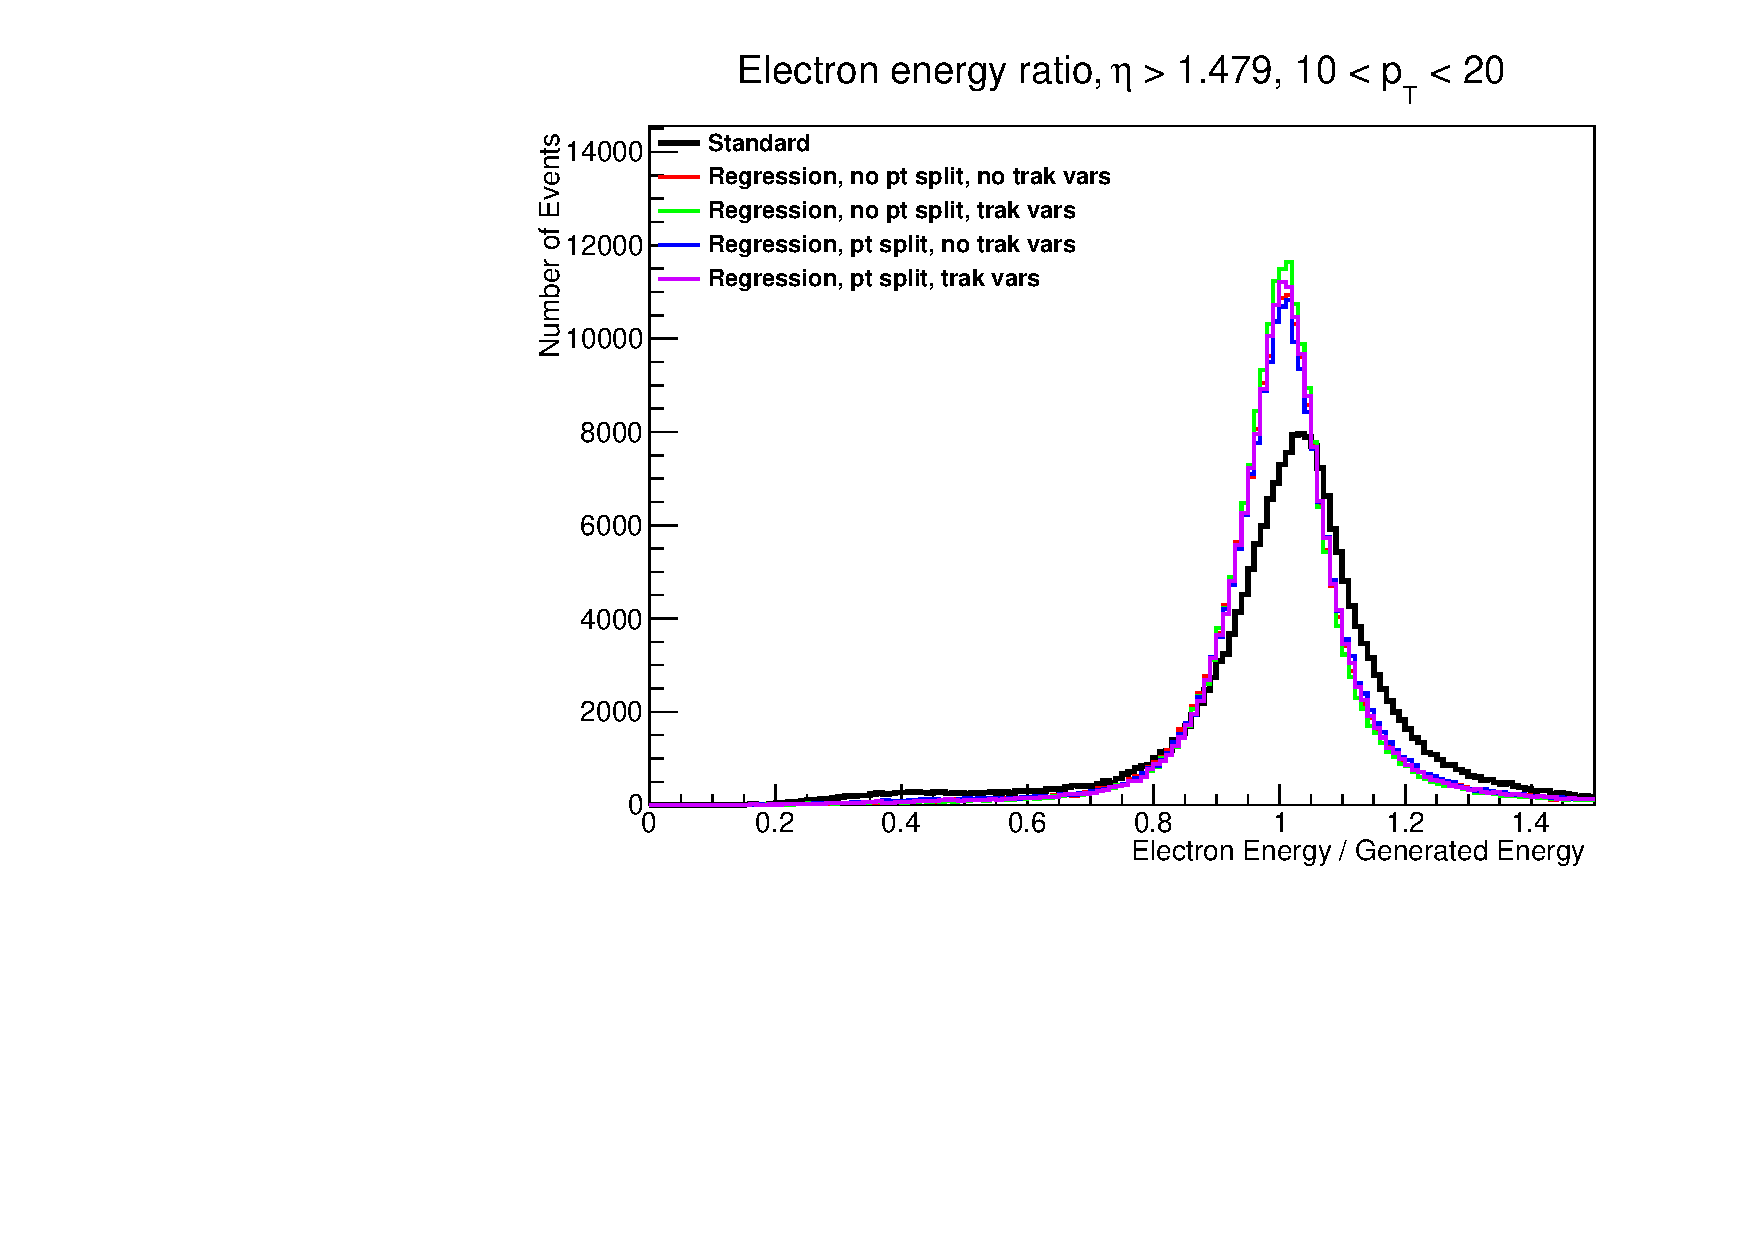
\includegraphics[width=0.6\textwidth]{figures/DY/EnergyResponse_allversions_binOption5.pdf}
		}
		\caption{Performance on Drell-Yan sample, medium $p_T$ bins}
		\label{fig:drellyanEnergyResponse2}
\end{figure}

\begin{figure}[h]
\centering
		\subfigure[]{
			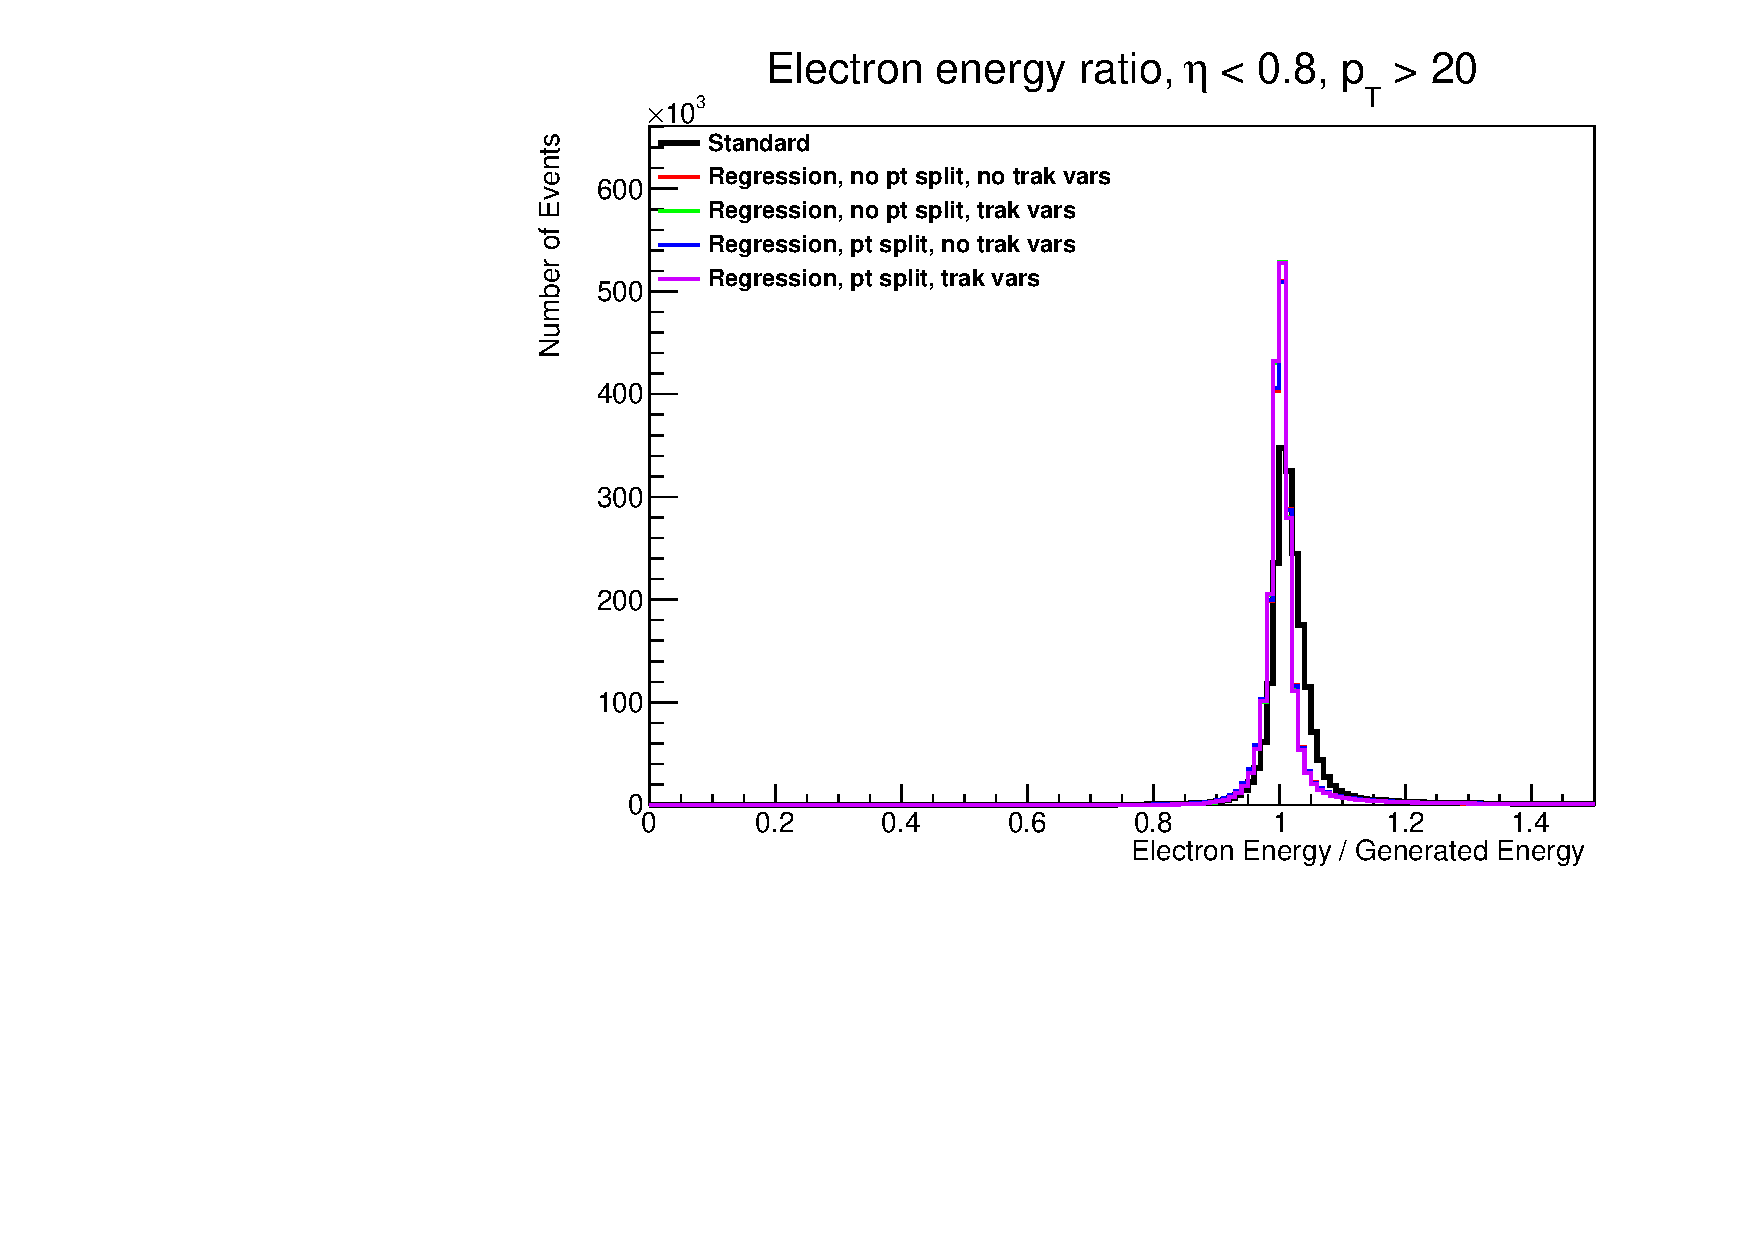
\includegraphics[width=0.6\textwidth]{figures/DY/EnergyResponse_allversions_binOption6.pdf}
		} \\
		\subfigure[]{
			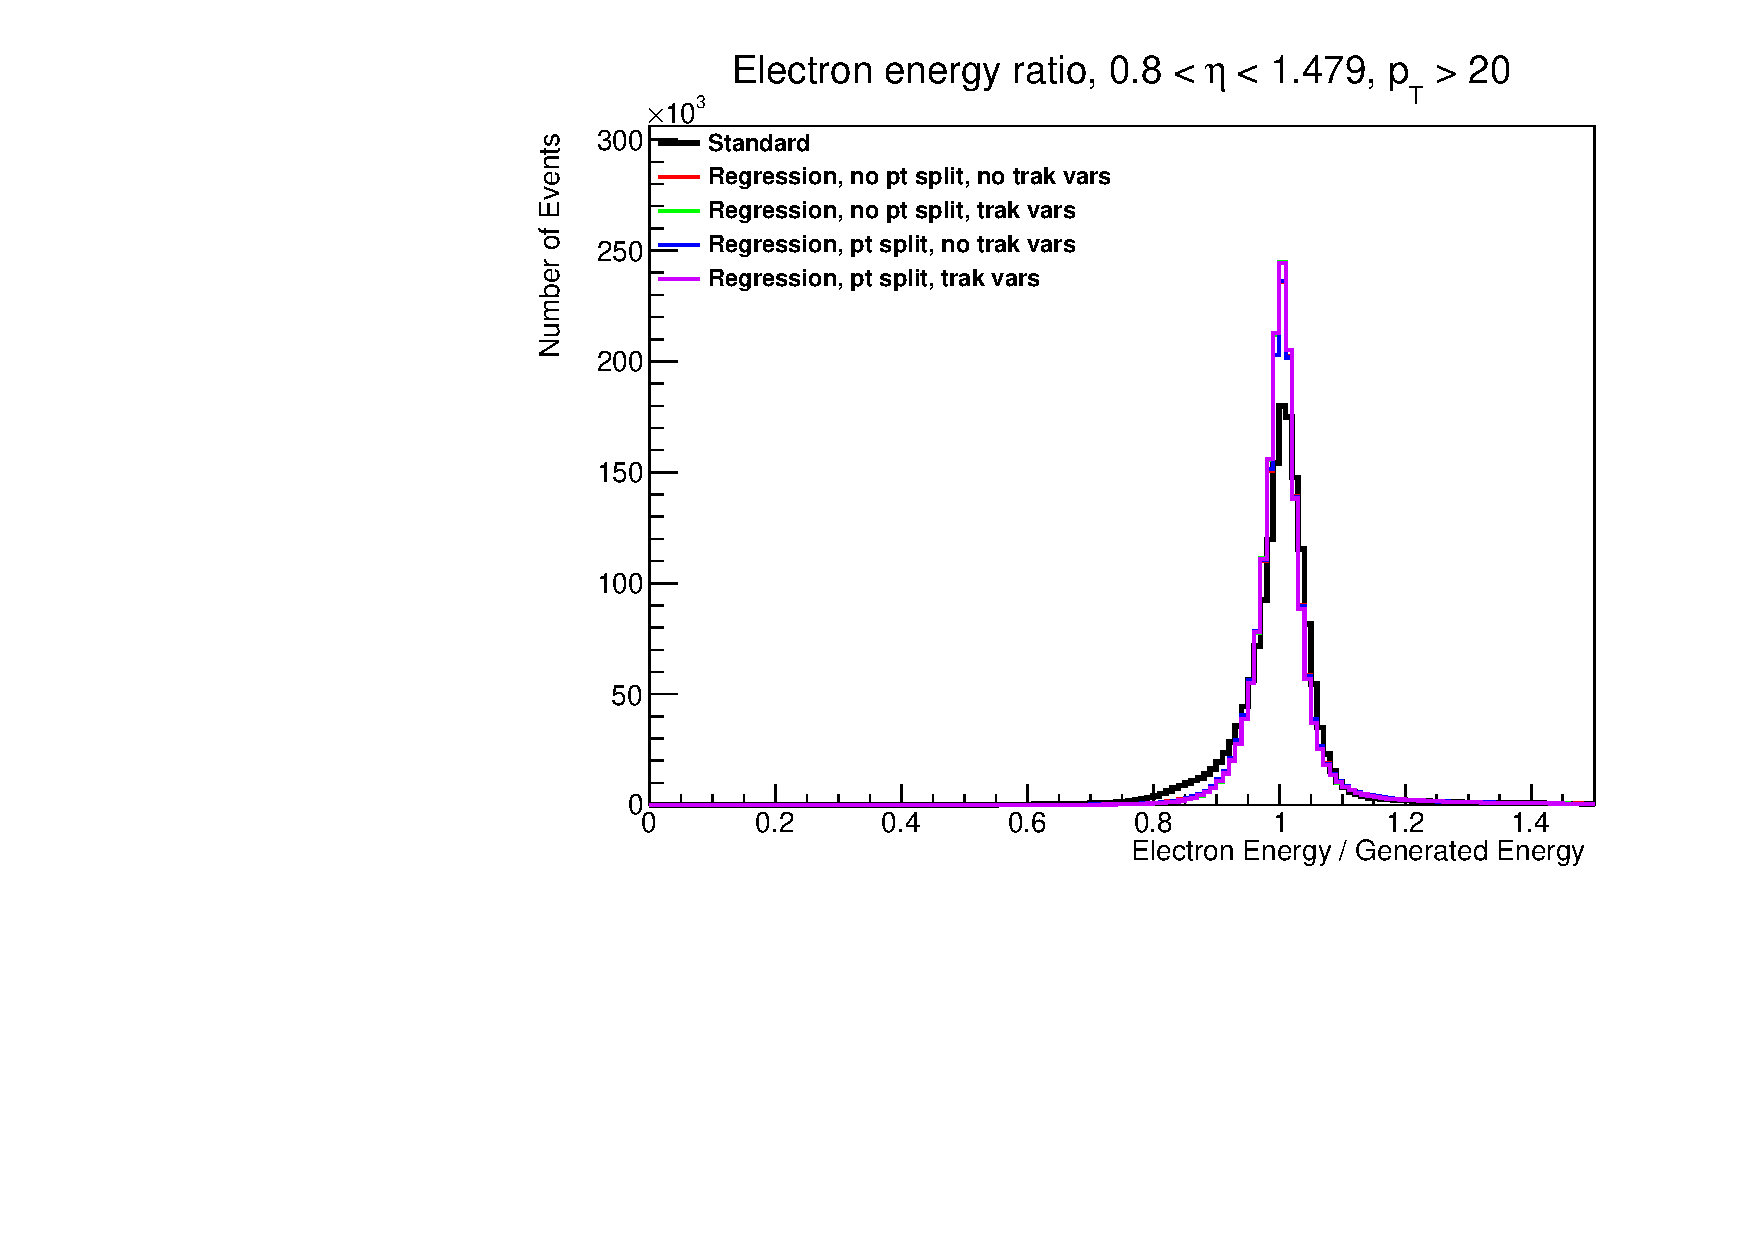
\includegraphics[width=0.6\textwidth]{figures/DY/EnergyResponse_allversions_binOption7.pdf}
		} \\
		\subfigure[]{
			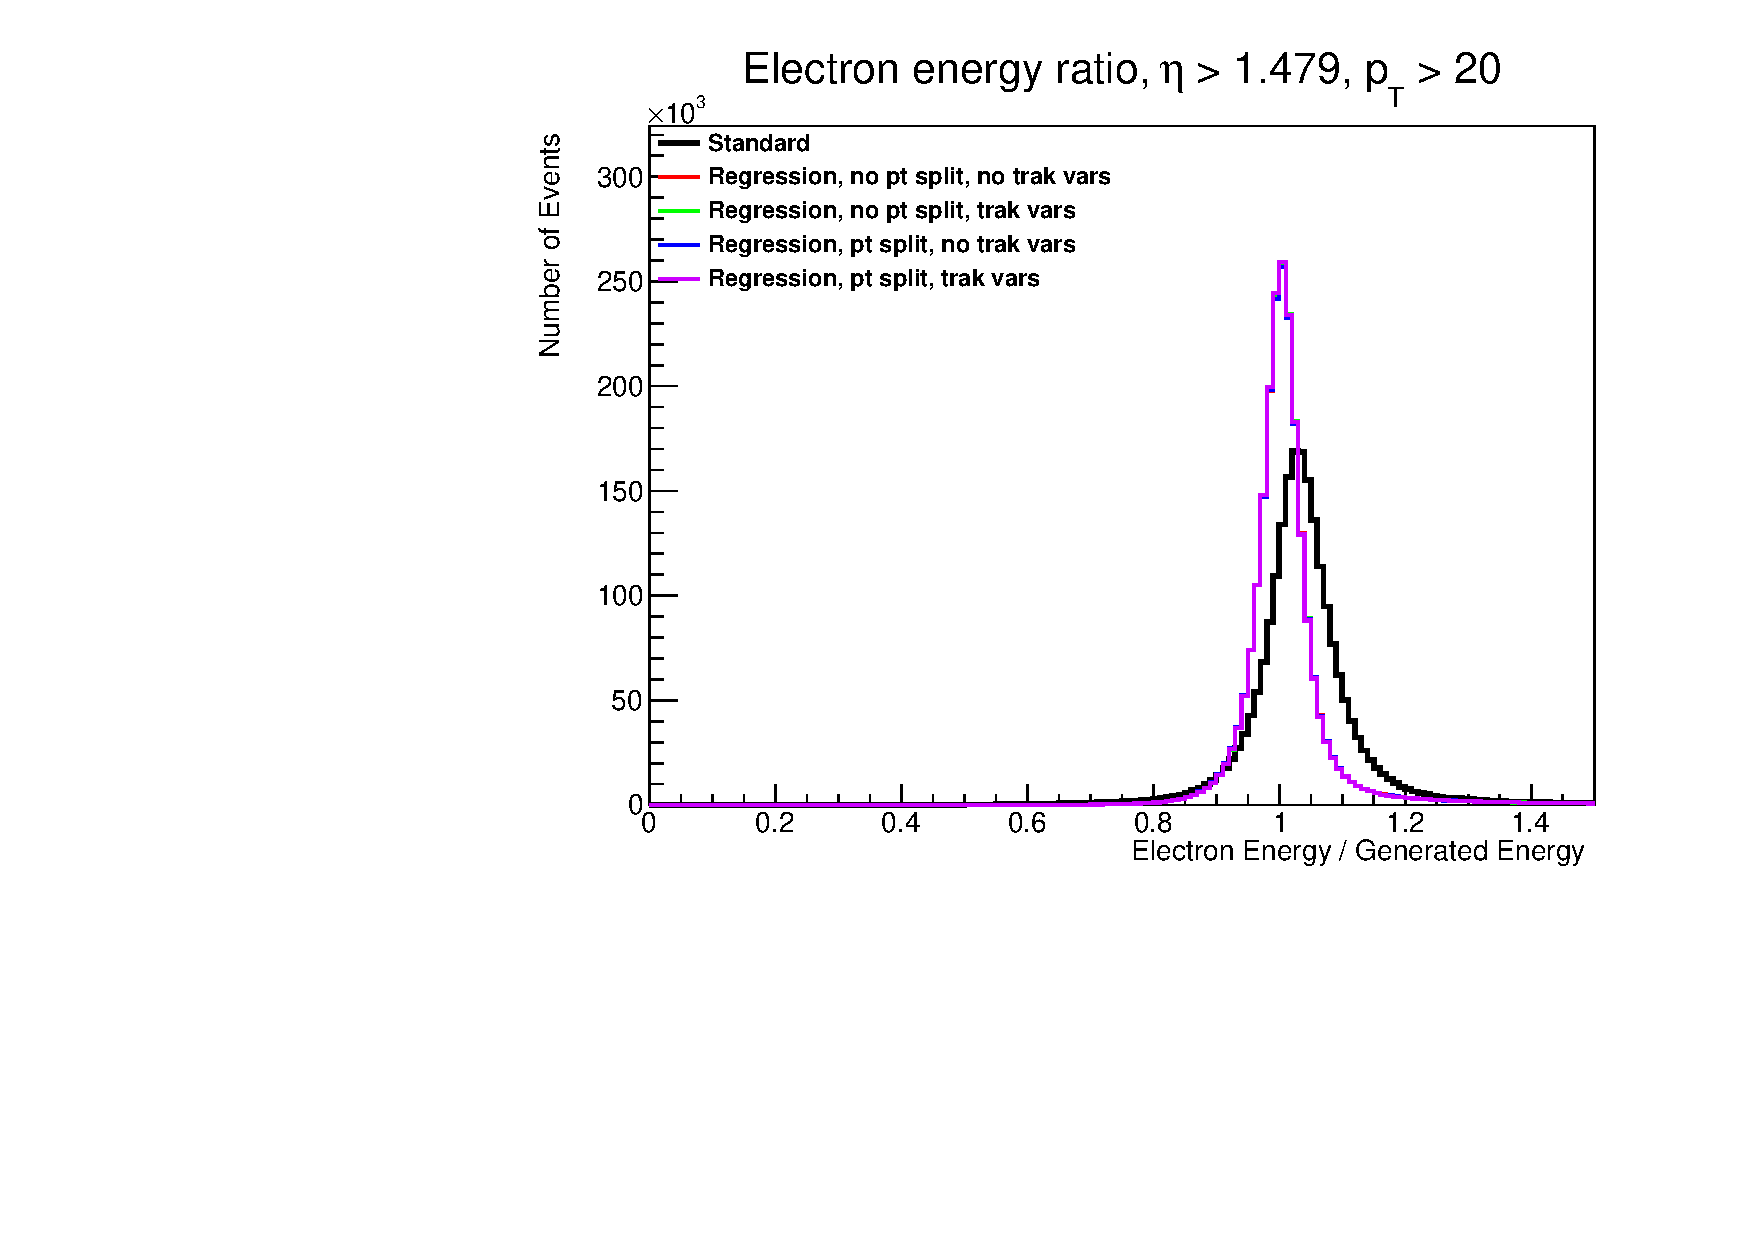
\includegraphics[width=0.6\textwidth]{figures/DY/EnergyResponse_allversions_binOption8.pdf}
		}
		\caption{Performance on Drell-Yan sample, high $p_T$ bins}
		\label{fig:drellyanEnergyResponse3}
\end{figure}


A number of general conclusions can be drawn from these comparisons. We observe that the regression energy calculation
significantly improves the energy resolution over the standard electron momentum reconstruction in all kinematic
regions with the exception of the barrel electrons in the lowest $p_{T}$ bin, where the inclusion of the momentum
uncertainty in the standard reconstruction may be yielding additional information not used in the regression. 
For the endcap, the standard reconstruction appears to systematically overestimate the electron energy, which
is corrected by the regression. We also observe that the inclusion of the
track-related variables in the regression significantly improves the energy resolution. 

Similar conclusions are drawn for the comparison using the Drell-Yan sample. 
The most significant additional feature is in the low-$p_T$, high-$\eta$ bins where
we observe a secondary peak and a significantly larger tail at low values of the
energy response. We hypothesize that these are highly radiative electrons, which are 
enhanced in the Drell-Yan sample by the fact that we are selecting a very specific
kinematic bin. 

We also observe that the regressions trained with two $p_T$ bins does not result in any 
significant improvement to the resolution, in almost all kinematic bins. The only
case where any improvement is observed is in the lowest $p_{T}$ barrel bin, without
the inclusion of track-related variables, where it is most likely that the difference
in the amount of bremstrahlung between low $p_{T}$ electrons and high $p_{T}$ electrons 
are partially captured by the explicit binning. The fact that no improvement is
observed when we use two $p_{T}$ bins in the case where track-related variables are 
included suggests that the multivariate regression algorithm is able to successfully
categorize these electrons and internally correct for any differences between electrons
in different $p_{T}$ regions.


In order to evaluate the sensitivity of the regression on sample composition, we also evaluated the performance
of the regression on a sample that is different from the one with which it was trained. The plots for the 
regressions trained on Higgs Signal and evaluated on Drell-Yan samples are shown in 
Figures \ref{fig:higgssignalCrossDrellyanEnergyResponse1}, \ref{fig:higgssignalCrossDrellyanEnergyResponse2}, and
\ref{fig:higgssignalCrossDrellyanEnergyResponse3}, and the plots for the regressions trained on the Drell-Yan sample
and evaluated on the \HiggsToZZ\ signal sample are shown in Figures \ref{fig:drellyanCrossHiggssignalPlots1},
\ref{fig:drellyanCrossHiggssignalPlots2}, and \ref{fig:drellyanCrossHiggssignalPlots3}. From these plots, we observe
that the performance of the regression is very similar when applied to an alternative Monte Carlo sample. This 
suggests that the performance of the regression is not particularly sensitive to the underlying physics process
which produce the electrons.  

%% Figures for cross HZZ4l x DY
\begin{figure}[h]
\centering
	\subfigure[]{
		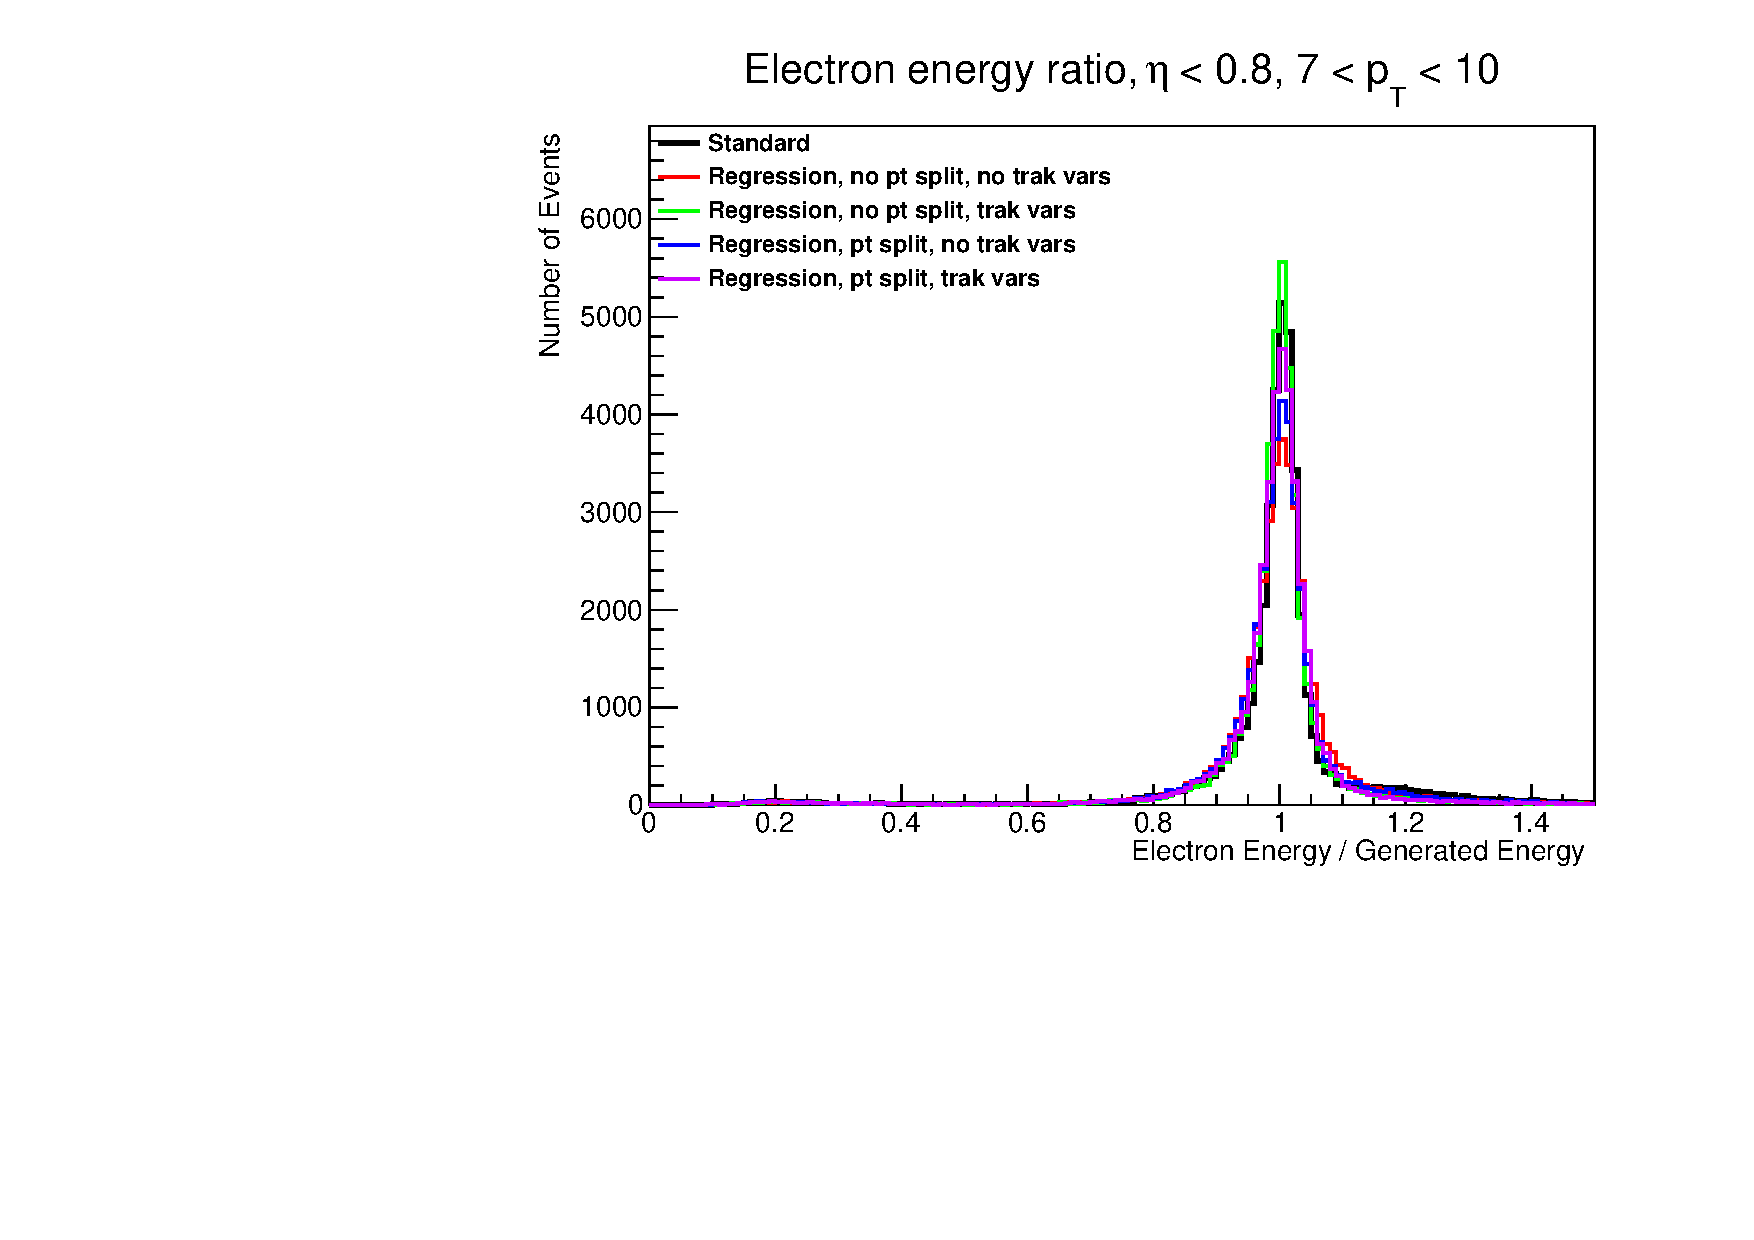
\includegraphics[width=0.6\textwidth]{figures/HZZ4l_cross_DY/EnergyResponse_allversions_binOption0.pdf}
	} \\
	\subfigure[]{
		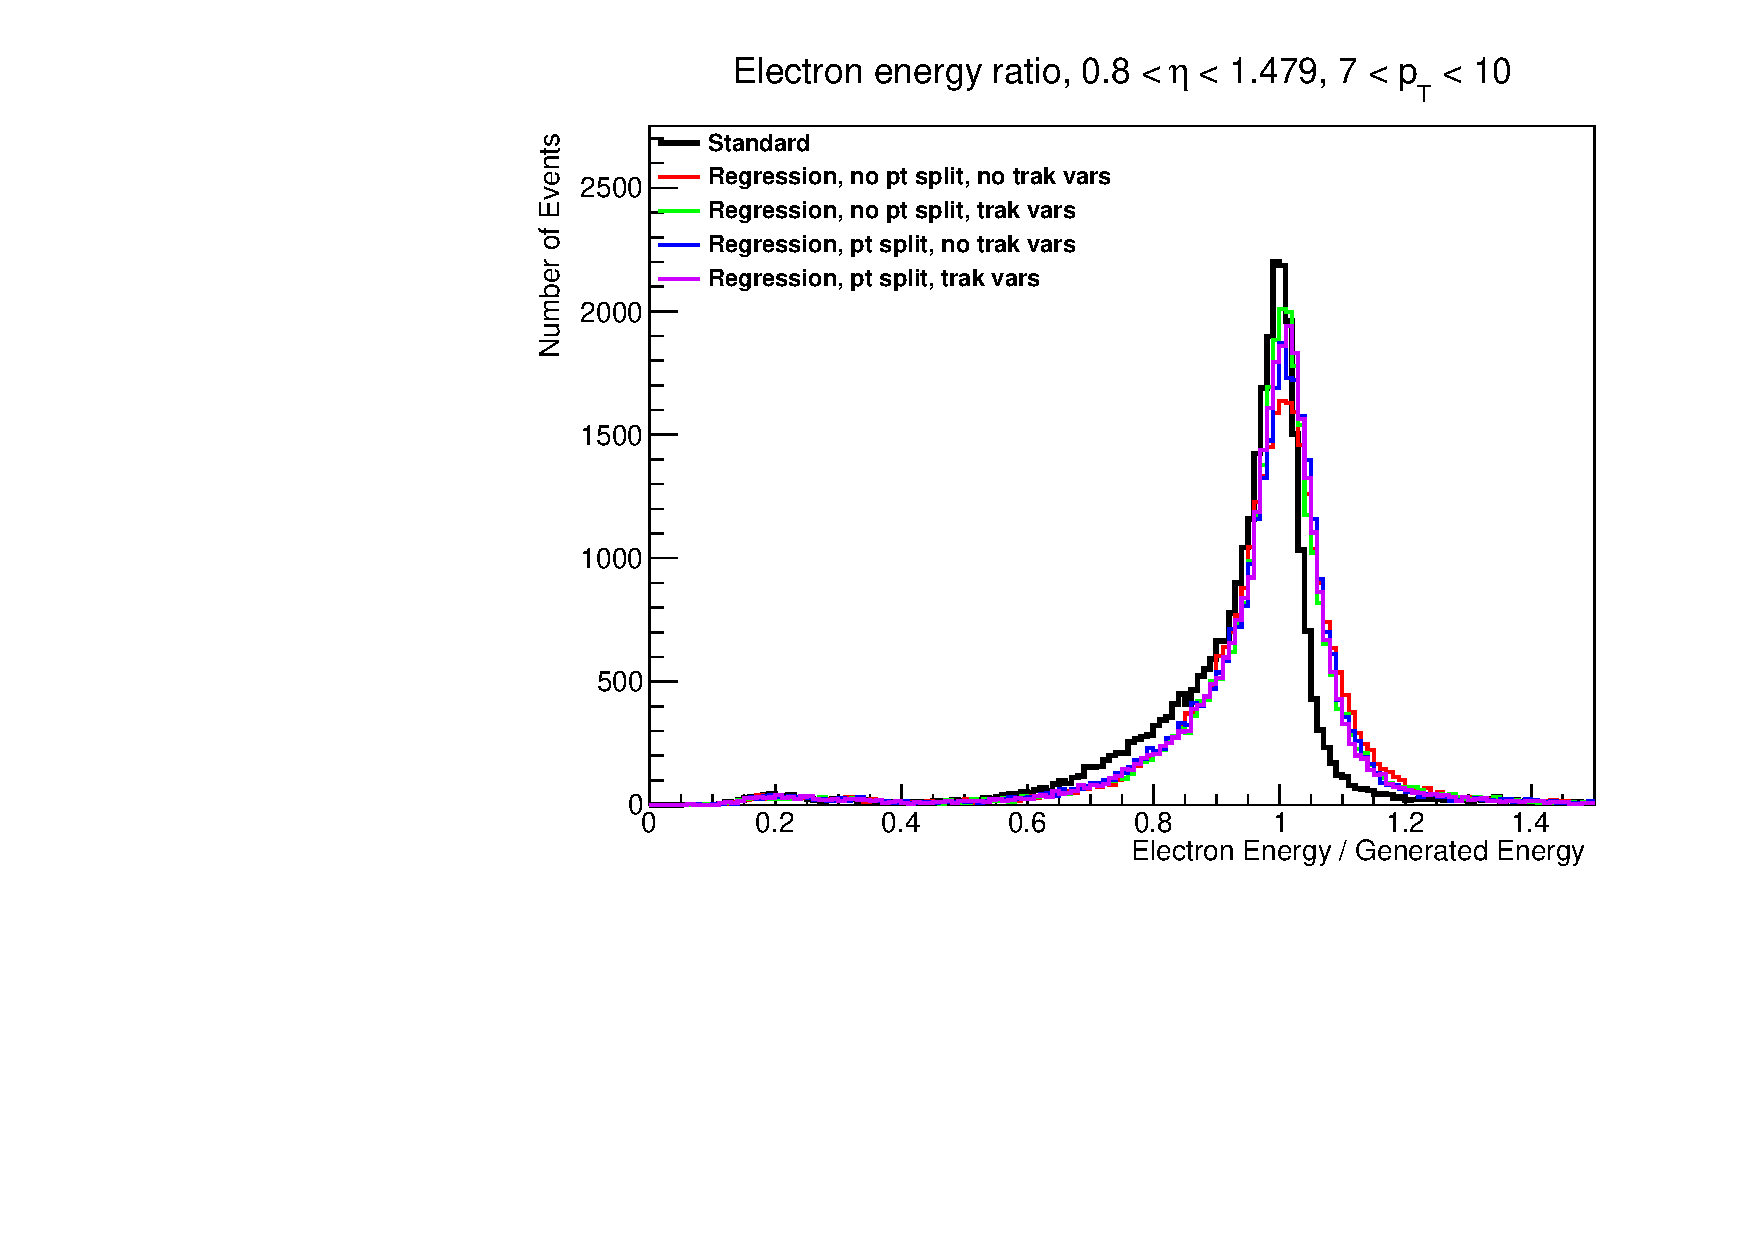
\includegraphics[width=0.6\textwidth]{figures/HZZ4l_cross_DY/EnergyResponse_allversions_binOption1.pdf}
	} \\
	\subfigure[]{
		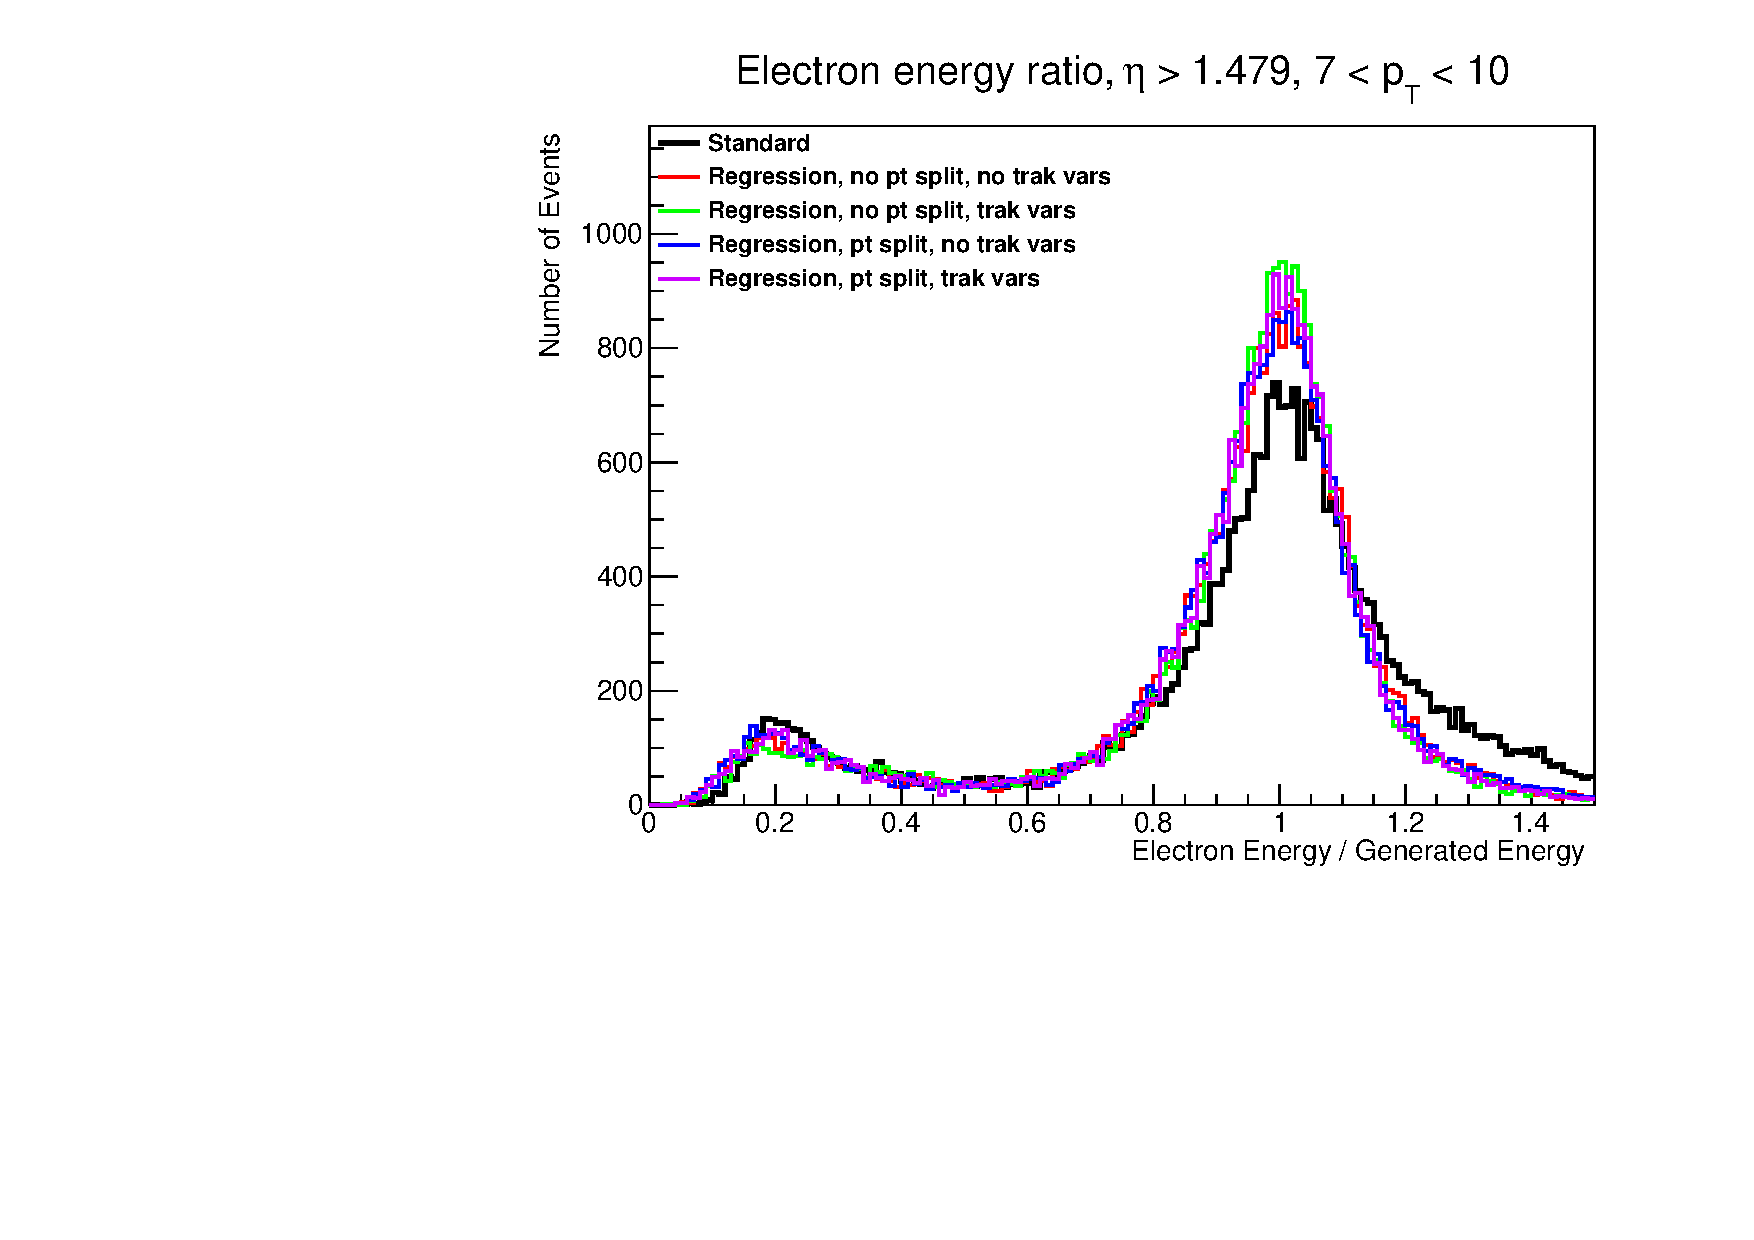
\includegraphics[width=0.6\textwidth]{figures/HZZ4l_cross_DY/EnergyResponse_allversions_binOption2.pdf}
	}
	\caption{Performance of regression trained on Higgs Signal and evaluated on Drell-Yan, low $p_T$ bins}
	\label{fig:higgssignalCrossDrellyanEnergyResponse1}
\end{figure}

\begin{figure}[h]
\centering
	\subfigure[]{
		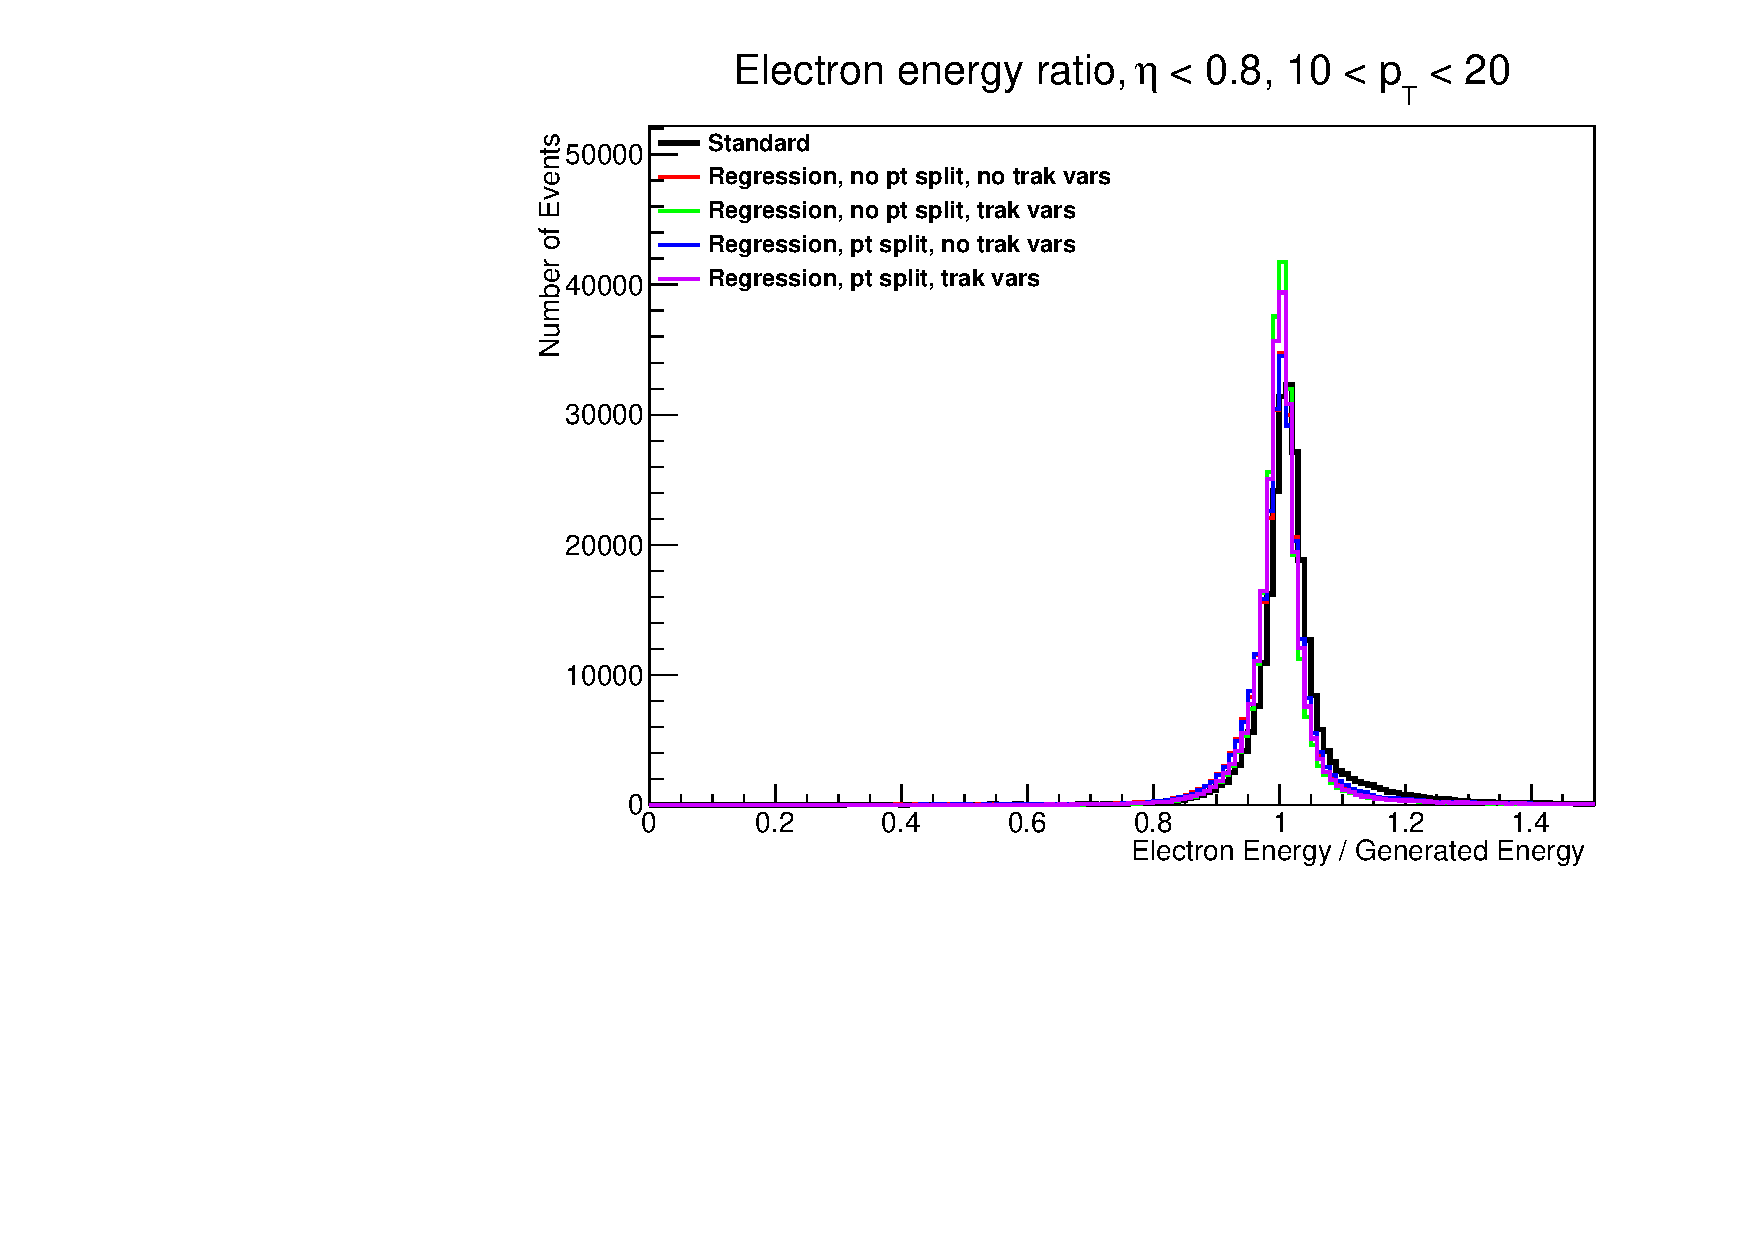
\includegraphics[width=0.6\textwidth]{figures/HZZ4l_cross_DY/EnergyResponse_allversions_binOption3.pdf}
	} \\
	\subfigure[]{
		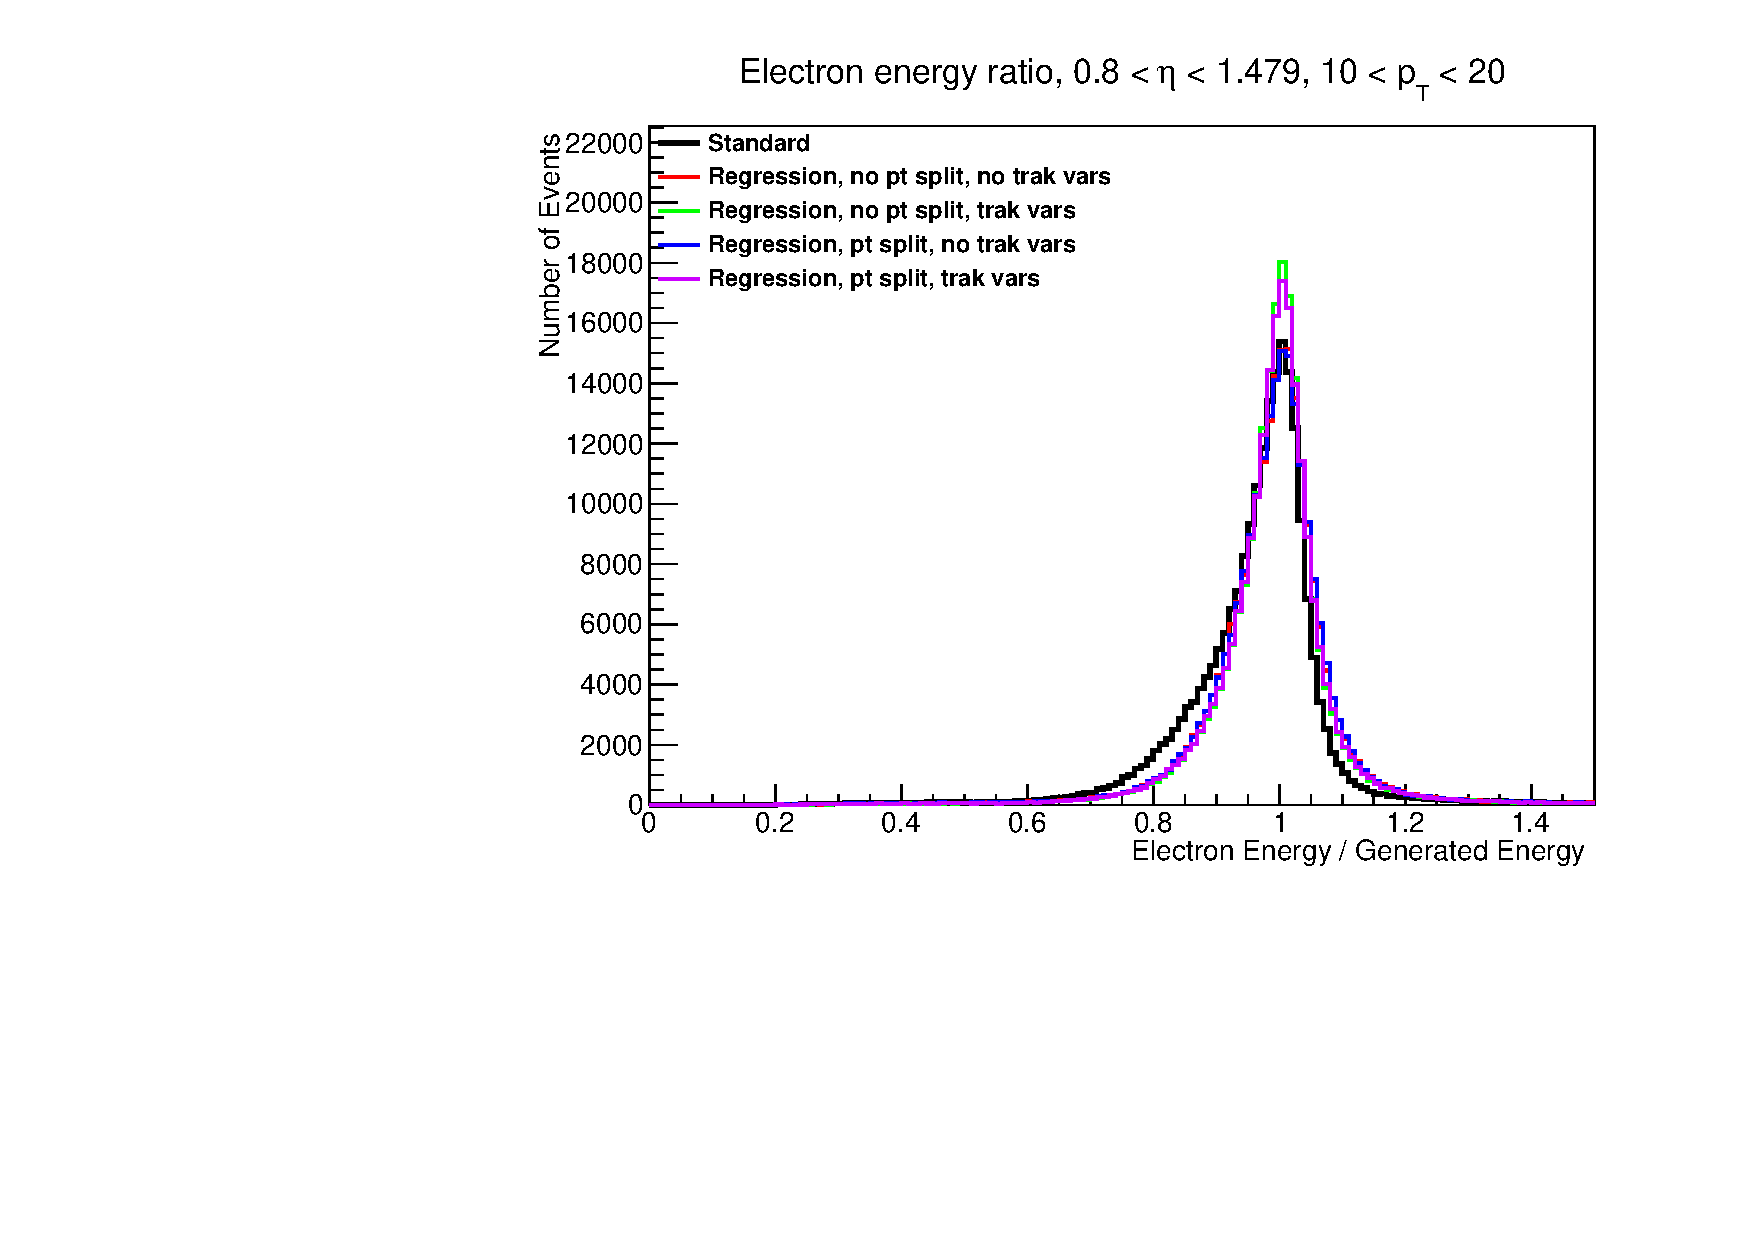
\includegraphics[width=0.6\textwidth]{figures/HZZ4l_cross_DY/EnergyResponse_allversions_binOption4.pdf}
	} \\
	\subfigure[]{
		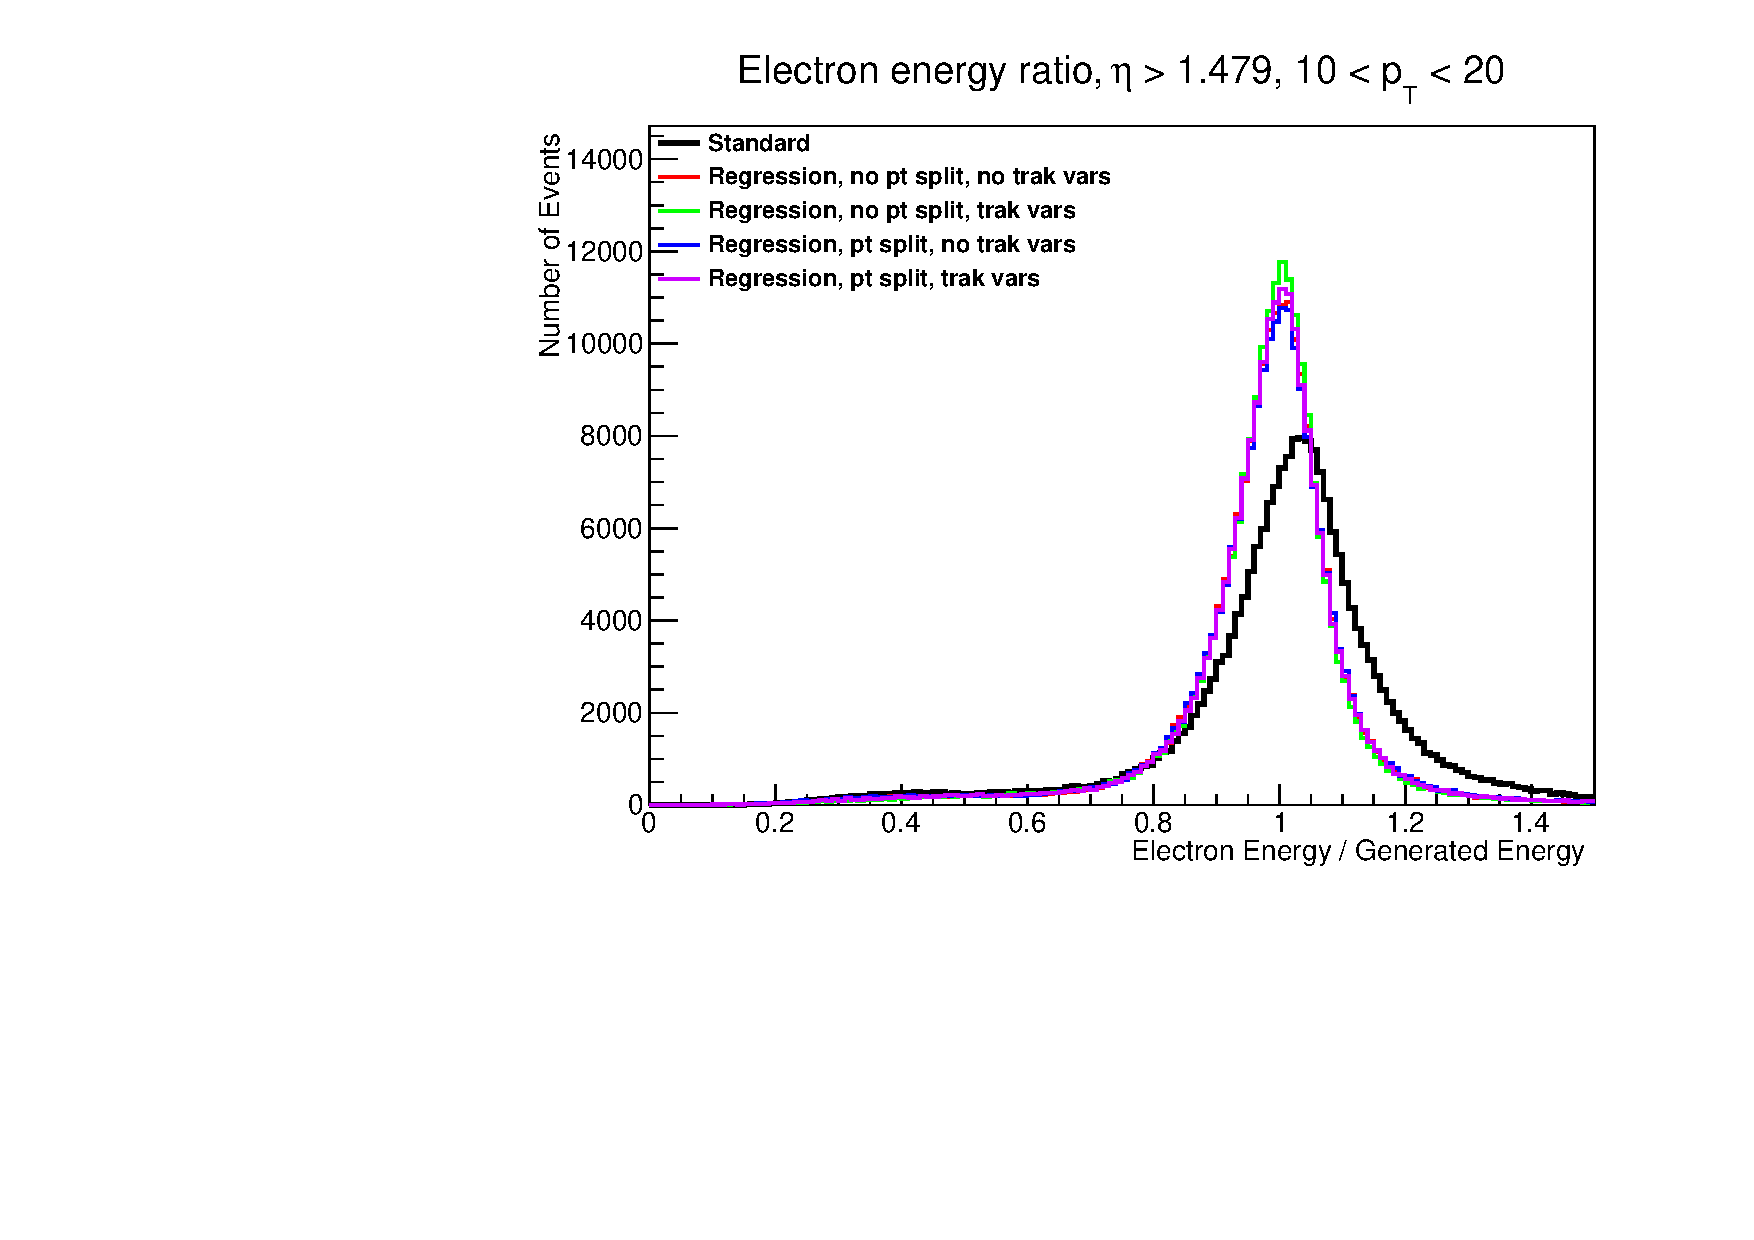
\includegraphics[width=0.6\textwidth]{figures/HZZ4l_cross_DY/EnergyResponse_allversions_binOption5.pdf}
	}
	\caption{Performance of regression trained on Higgs Signal and evaluated on Drell-Yan, medium $p_T$ bins}
	\label{fig:higgssignalCrossDrellyanEnergyResponse2}
\end{figure}

\begin{figure}[h]
\centering
	\subfigure[]{
		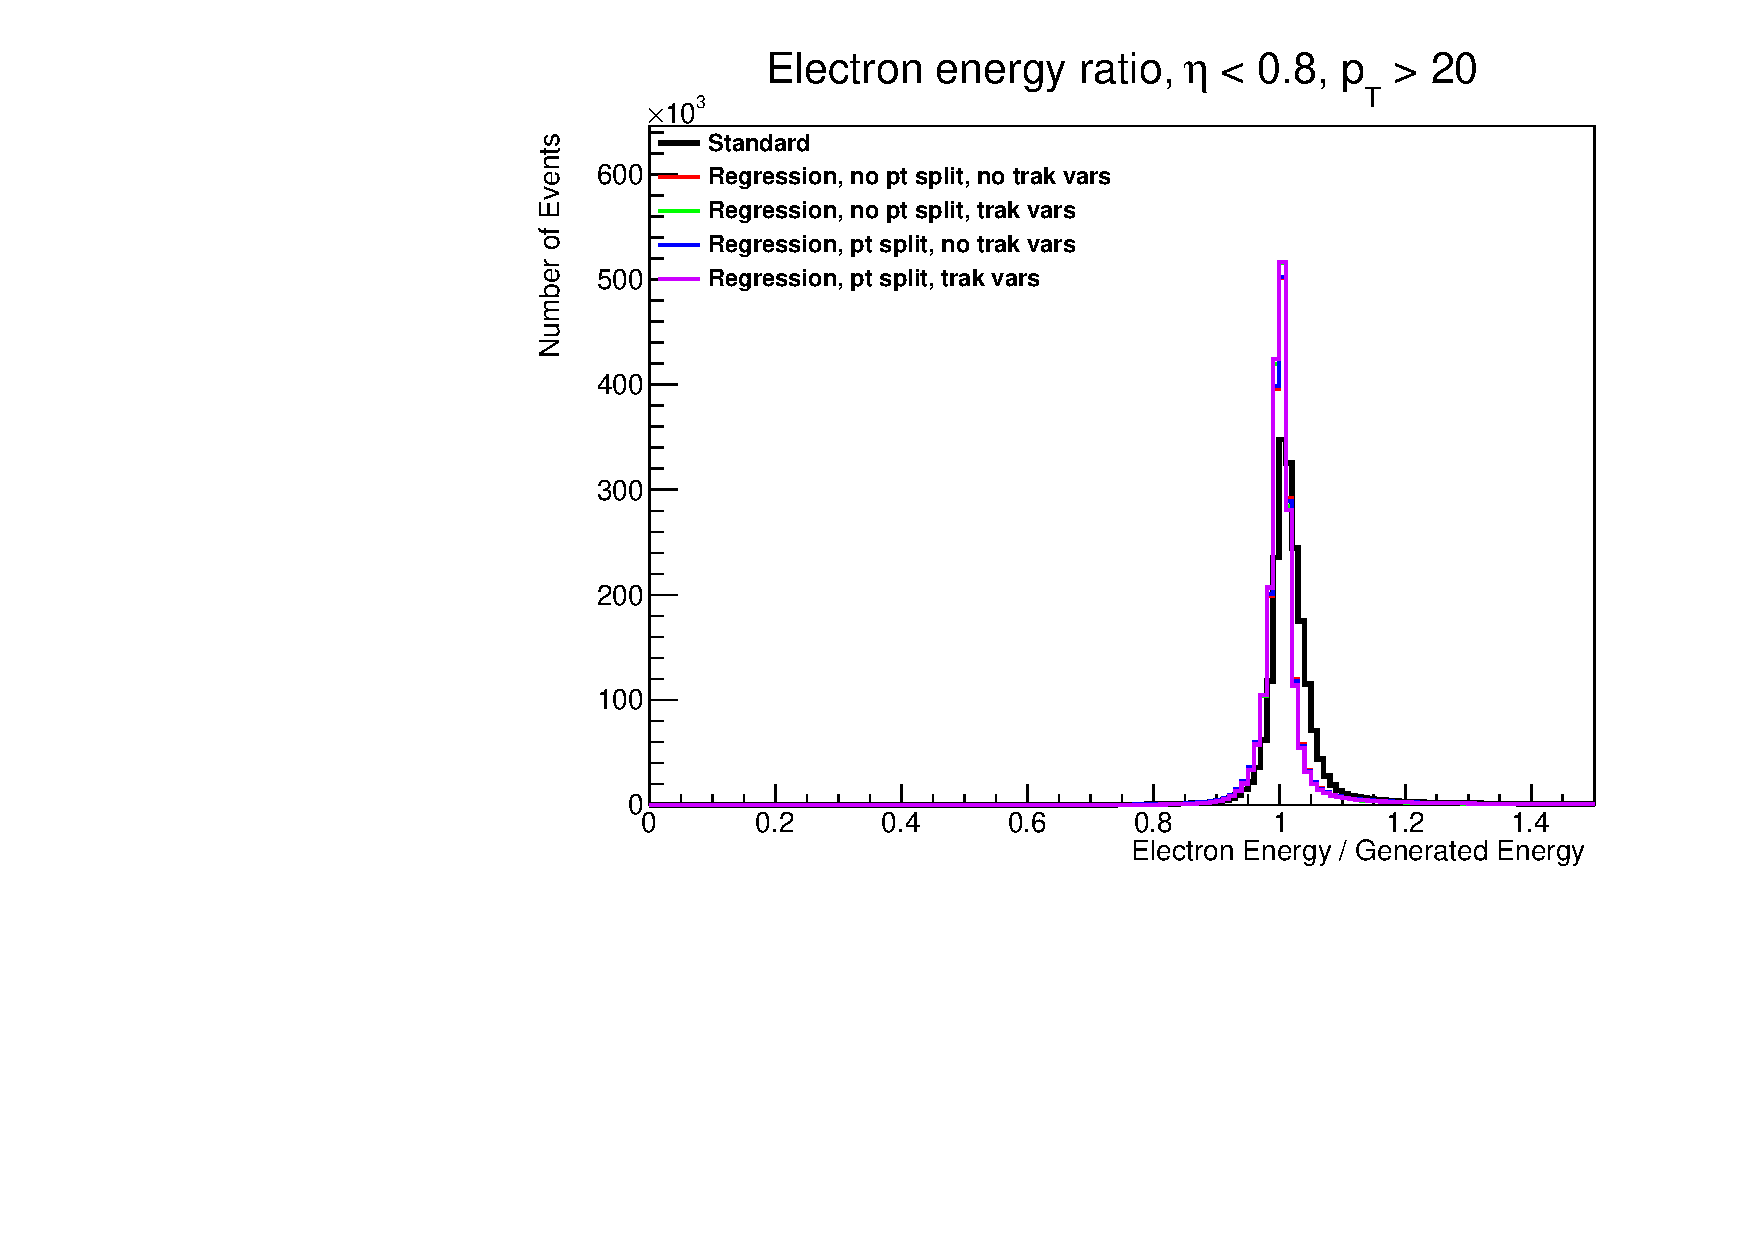
\includegraphics[width=0.6\textwidth]{figures/HZZ4l_cross_DY/EnergyResponse_allversions_binOption6.pdf}
	} \\
	\subfigure[]{
		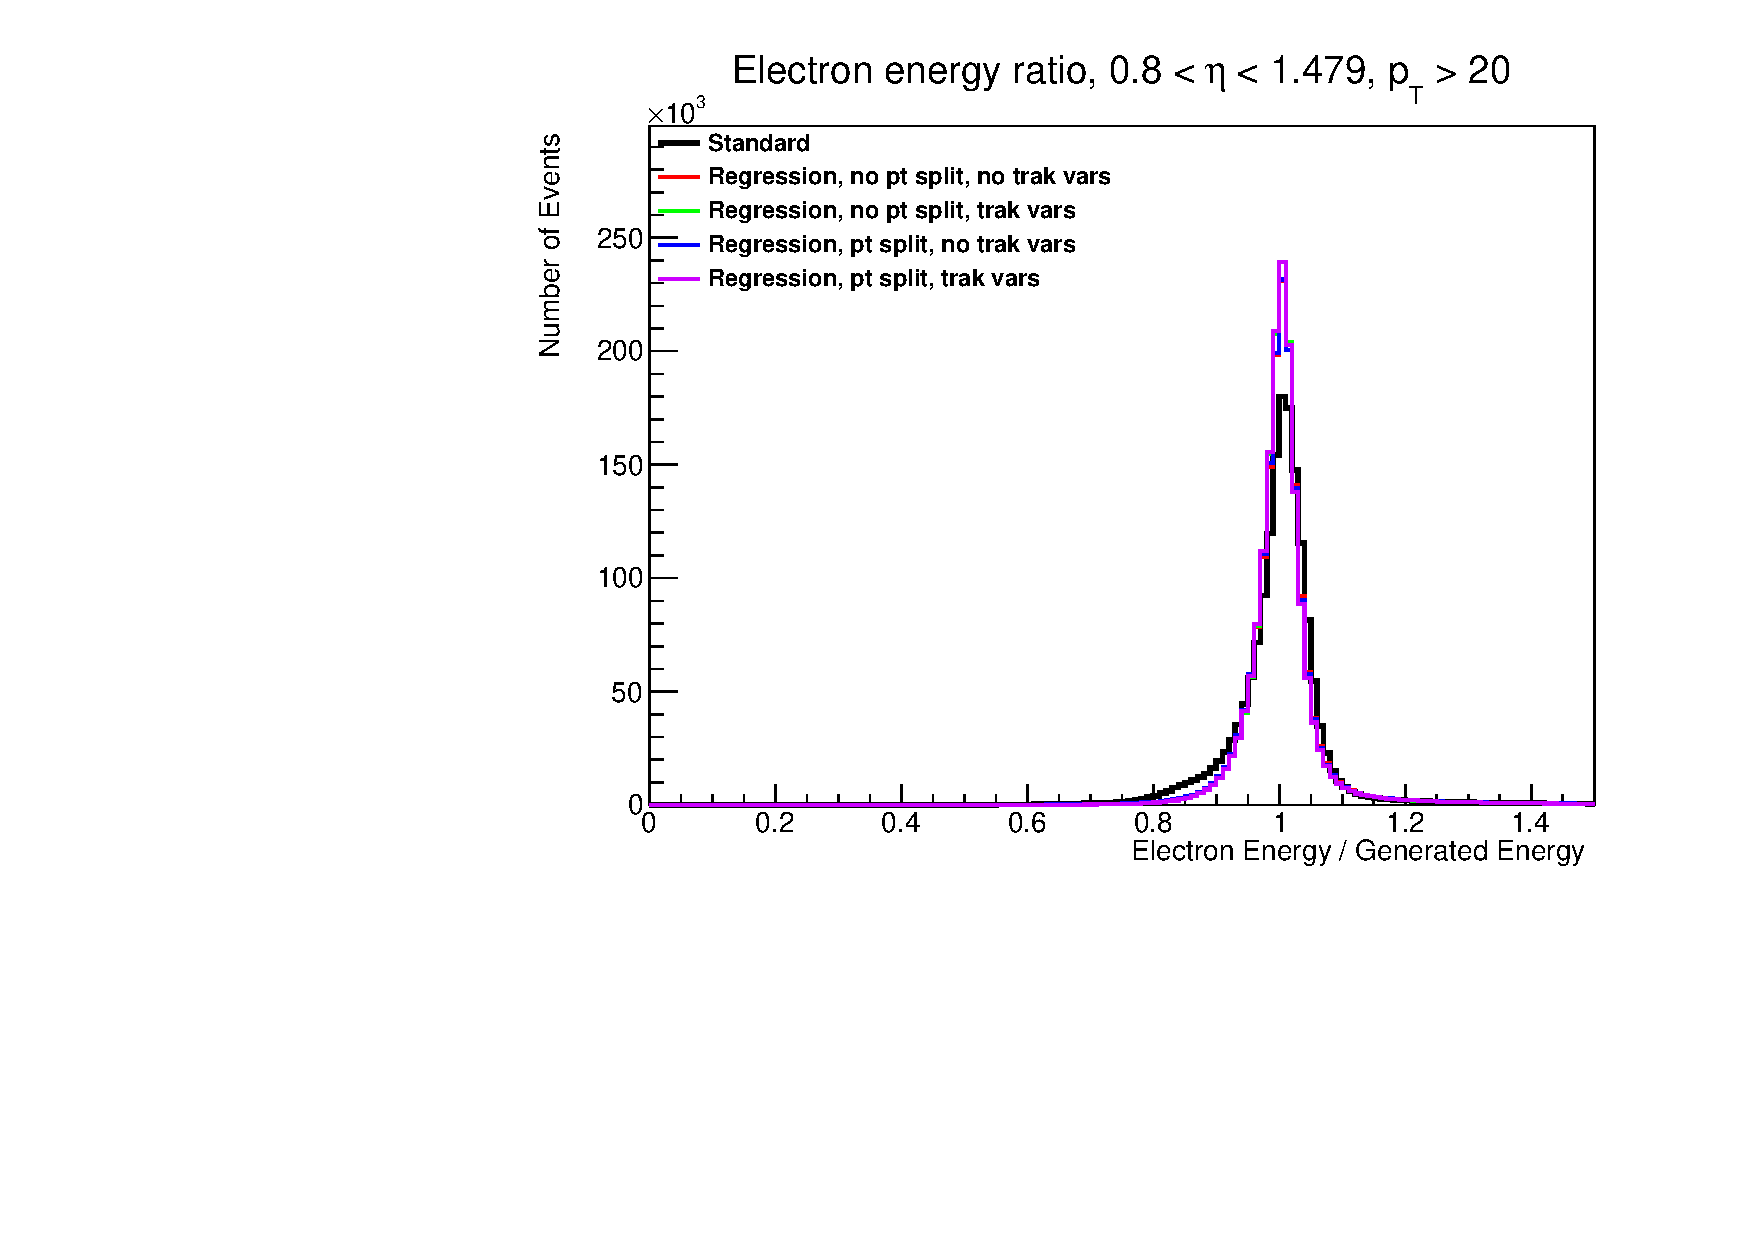
\includegraphics[width=0.6\textwidth]{figures/HZZ4l_cross_DY/EnergyResponse_allversions_binOption7.pdf}
	} \\
	\subfigure[]{
		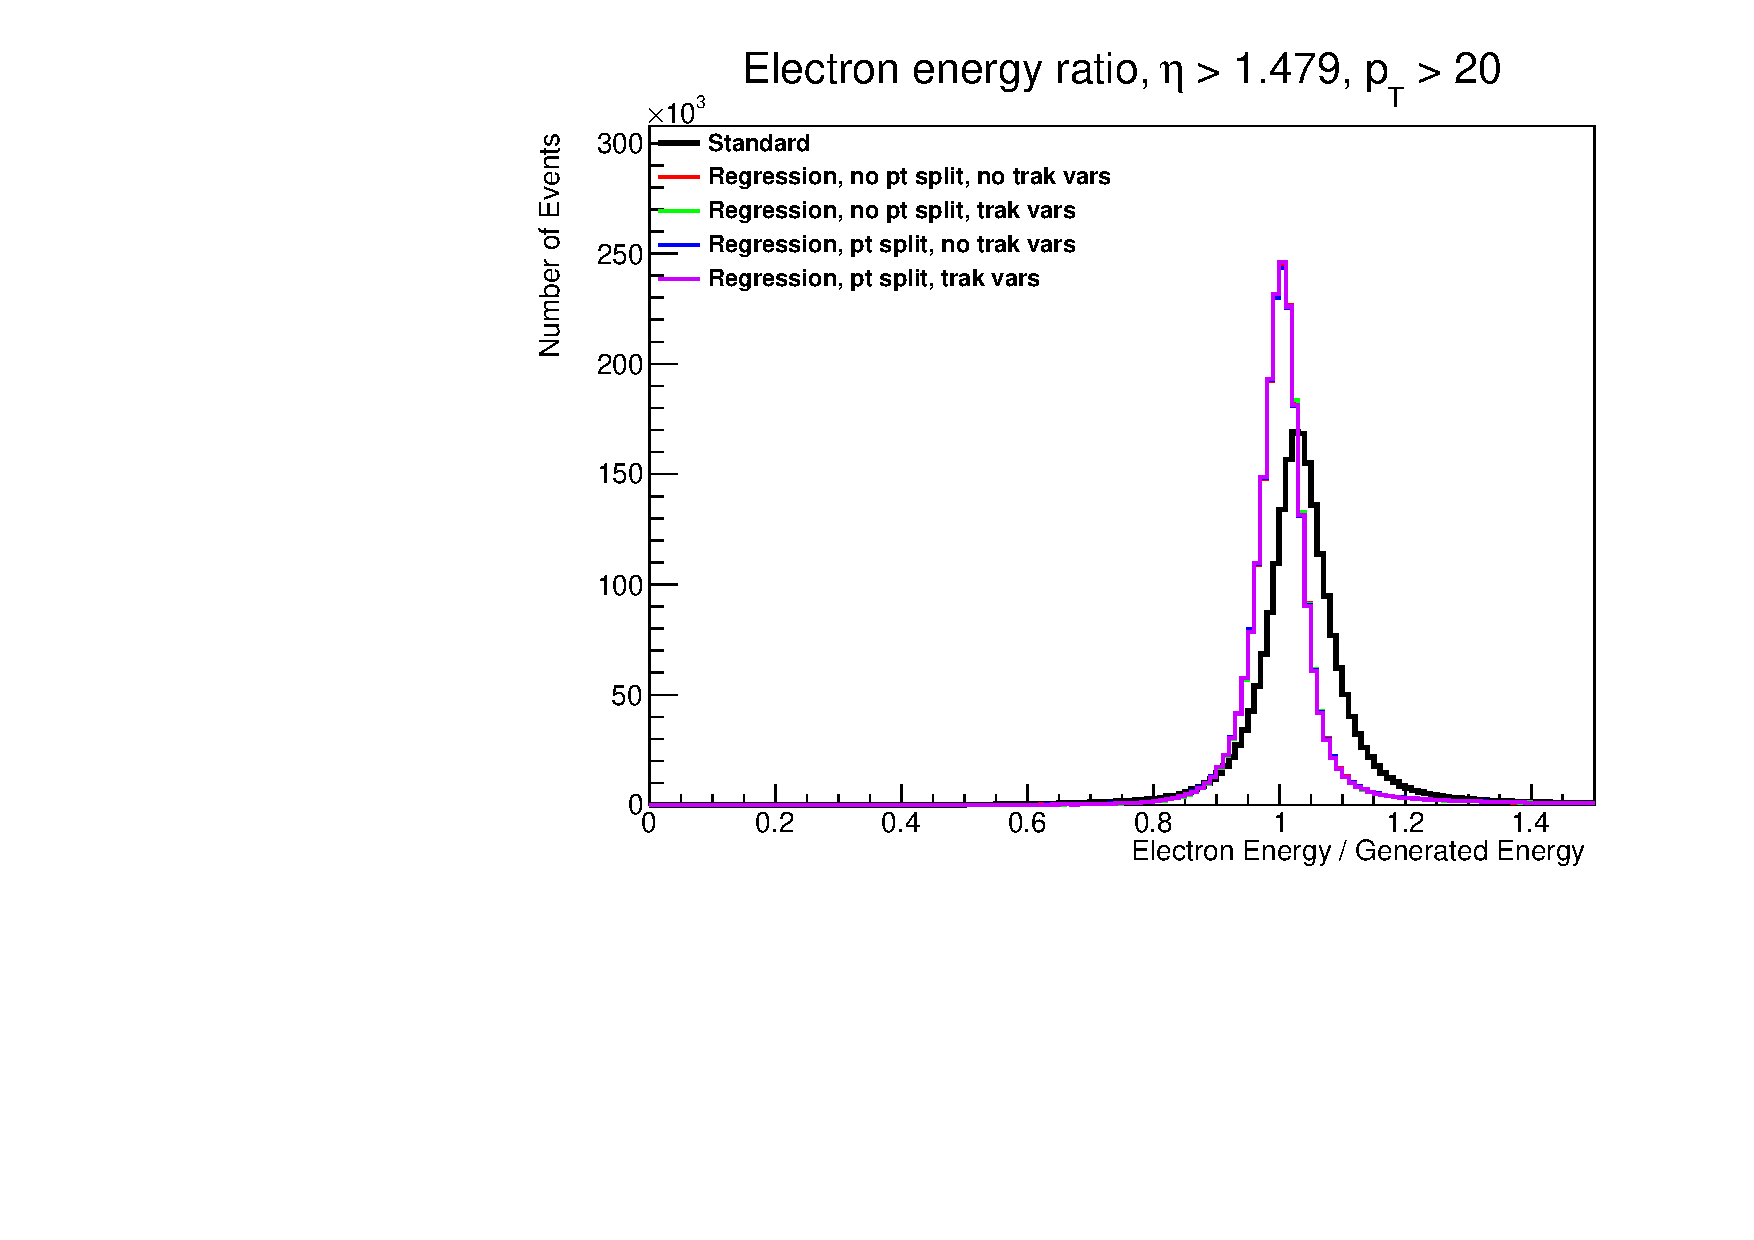
\includegraphics[width=0.6\textwidth]{figures/HZZ4l_cross_DY/EnergyResponse_allversions_binOption8.pdf}
	}
	\caption{Performance of regression trained on Higgs Signal and evaluated on Drell-Yan, high $p_T$ bins}
	\label{fig:higgssignalCrossDrellyanEnergyResponse3}
\end{figure}

%% Figures for cross DY x HZZ4l
\begin{figure}[h]
\centering
	\subfigure[]{
		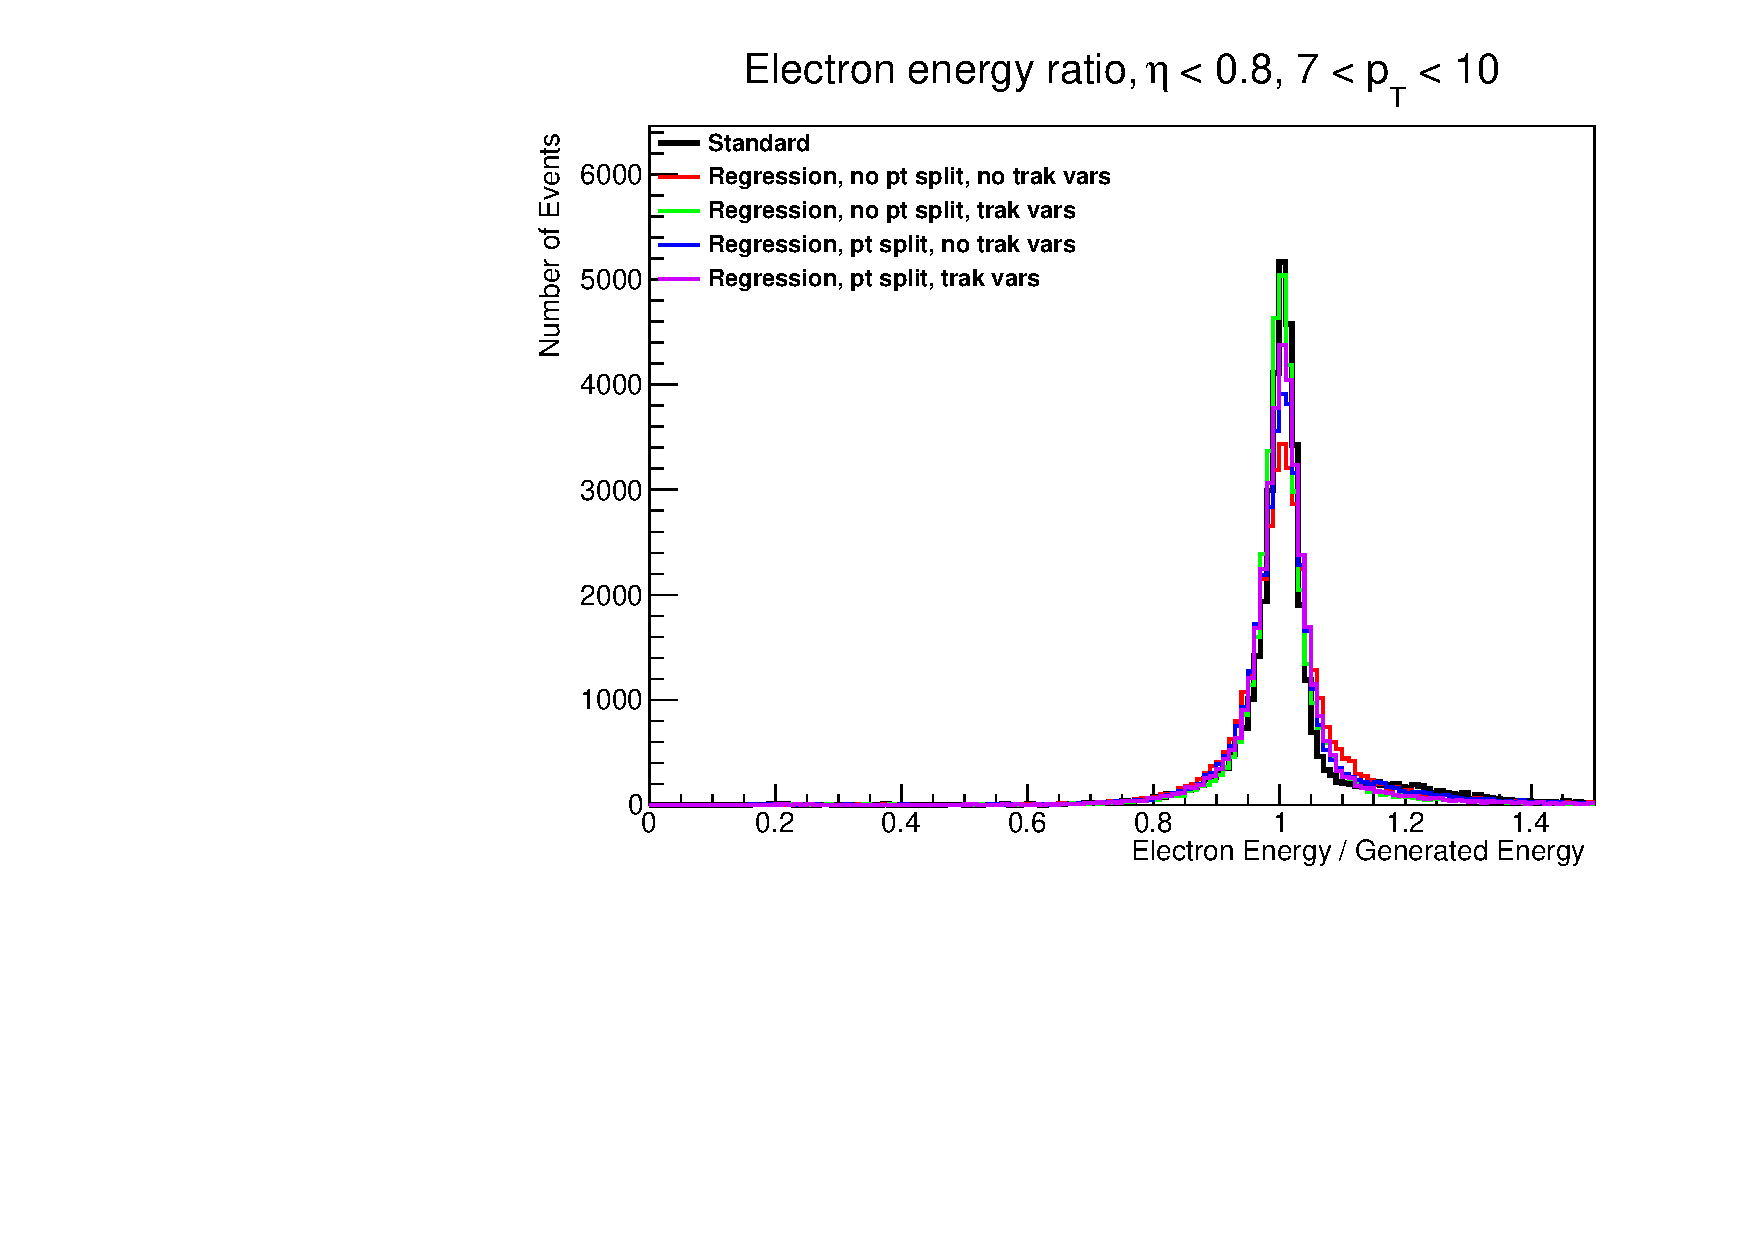
\includegraphics[width=0.6\textwidth]{figures/DY_cross_HZZ4l/EnergyResponse_allversions_binOption0.pdf}
	} \\
	\subfigure[]{
		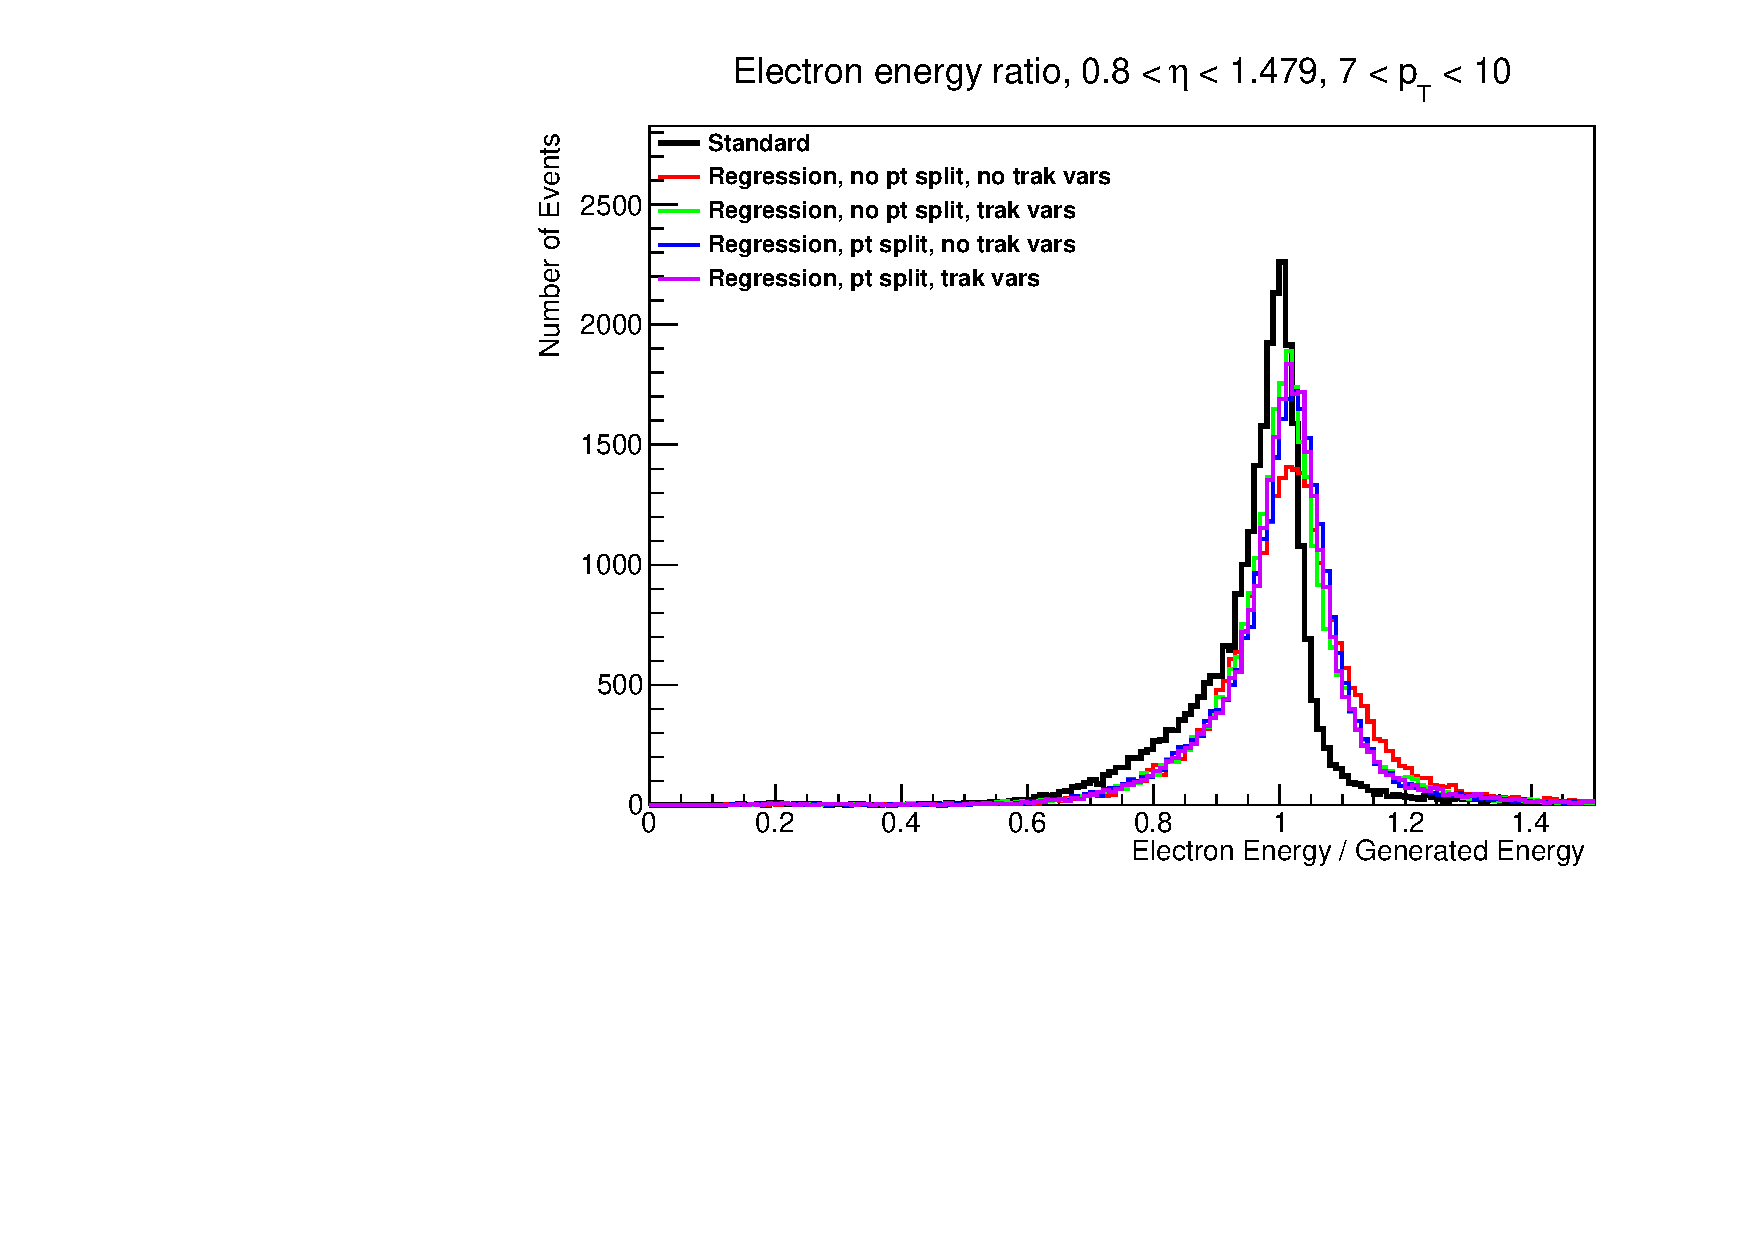
\includegraphics[width=0.6\textwidth]{figures/DY_cross_HZZ4l/EnergyResponse_allversions_binOption1.pdf}
	} \\
	\subfigure[]{
		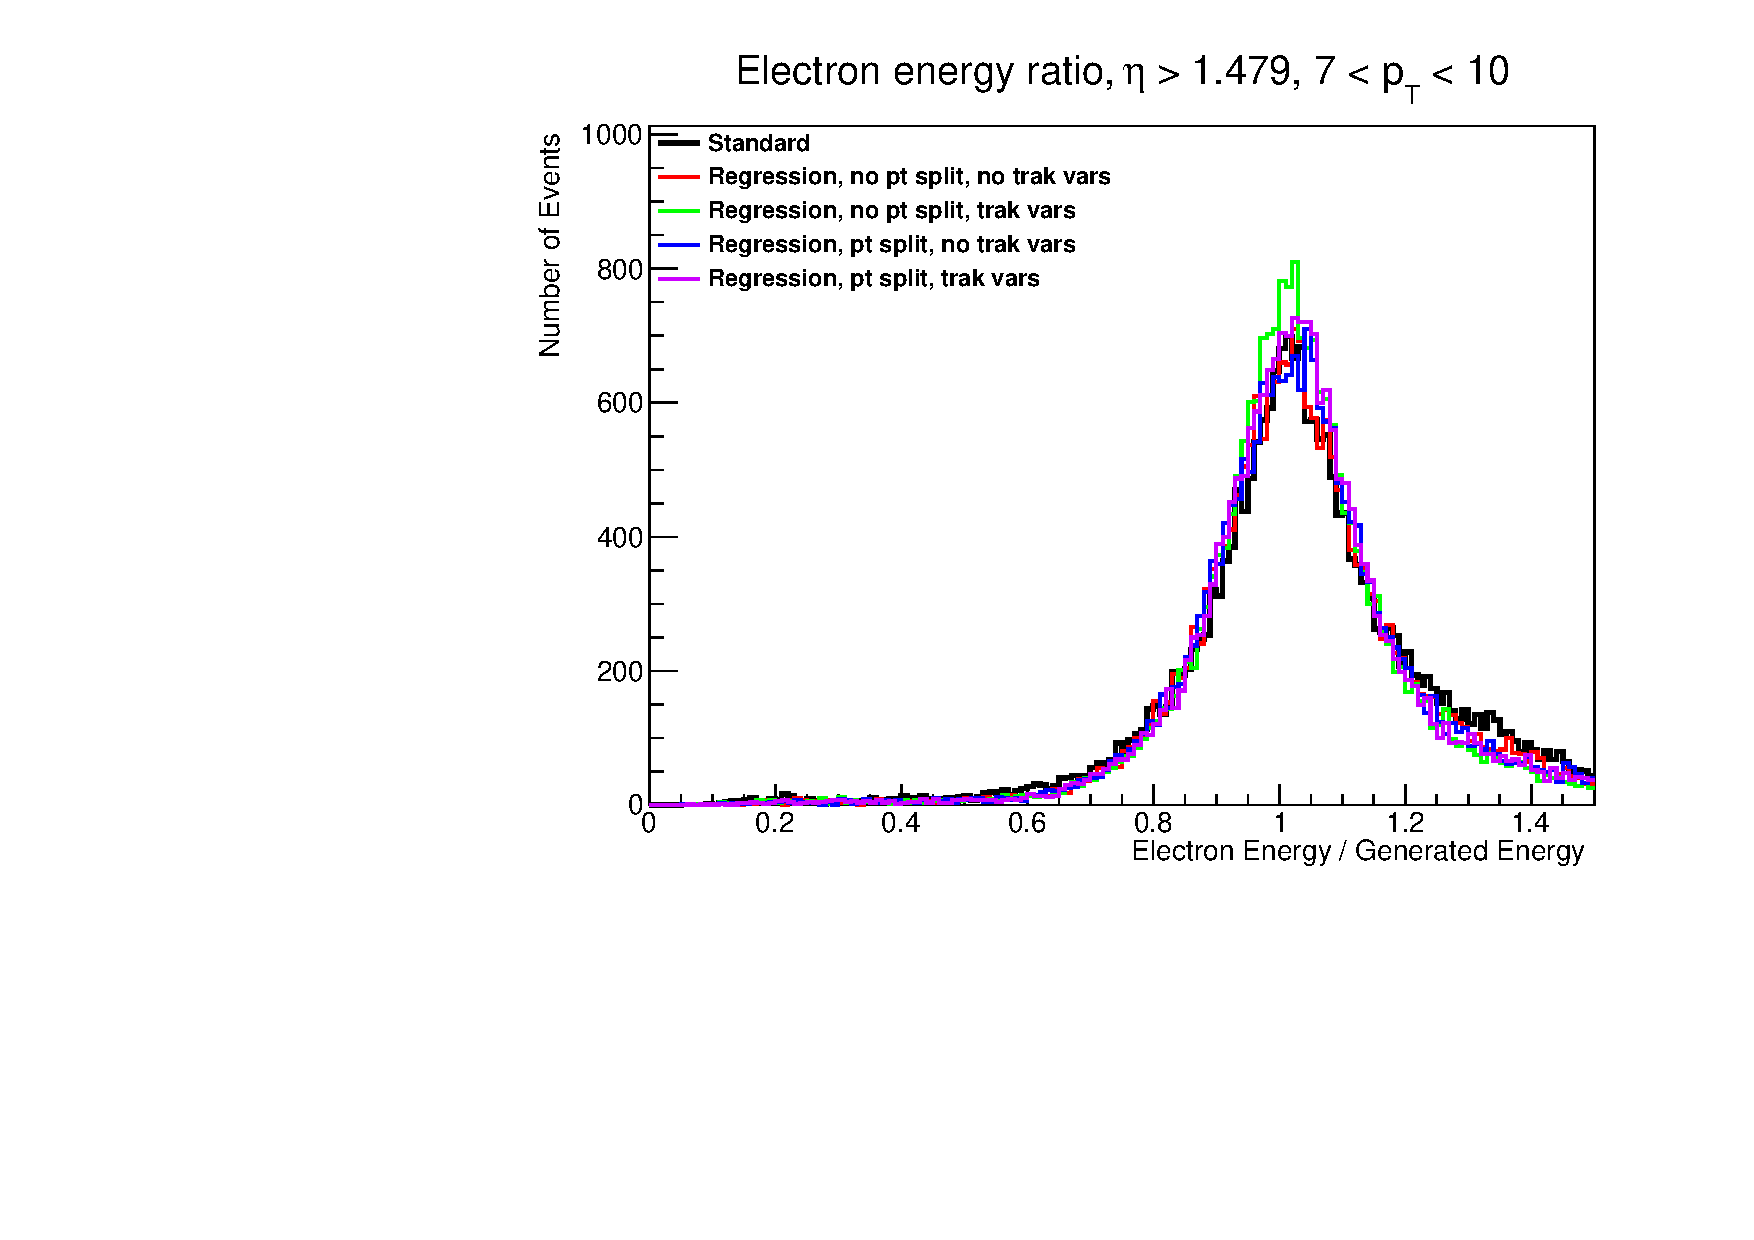
\includegraphics[width=0.6\textwidth]{figures/DY_cross_HZZ4l/EnergyResponse_allversions_binOption2.pdf}
	}
	\caption{Performance of regression trained on Drell-Yan and evaluated on Higgs Signal, low $p_T$ bins}
	\label{fig:drellyanCrossHiggssignalEnergyResponse1}
\end{figure}

\begin{figure}[h]
\centering
	\subfigure[]{
		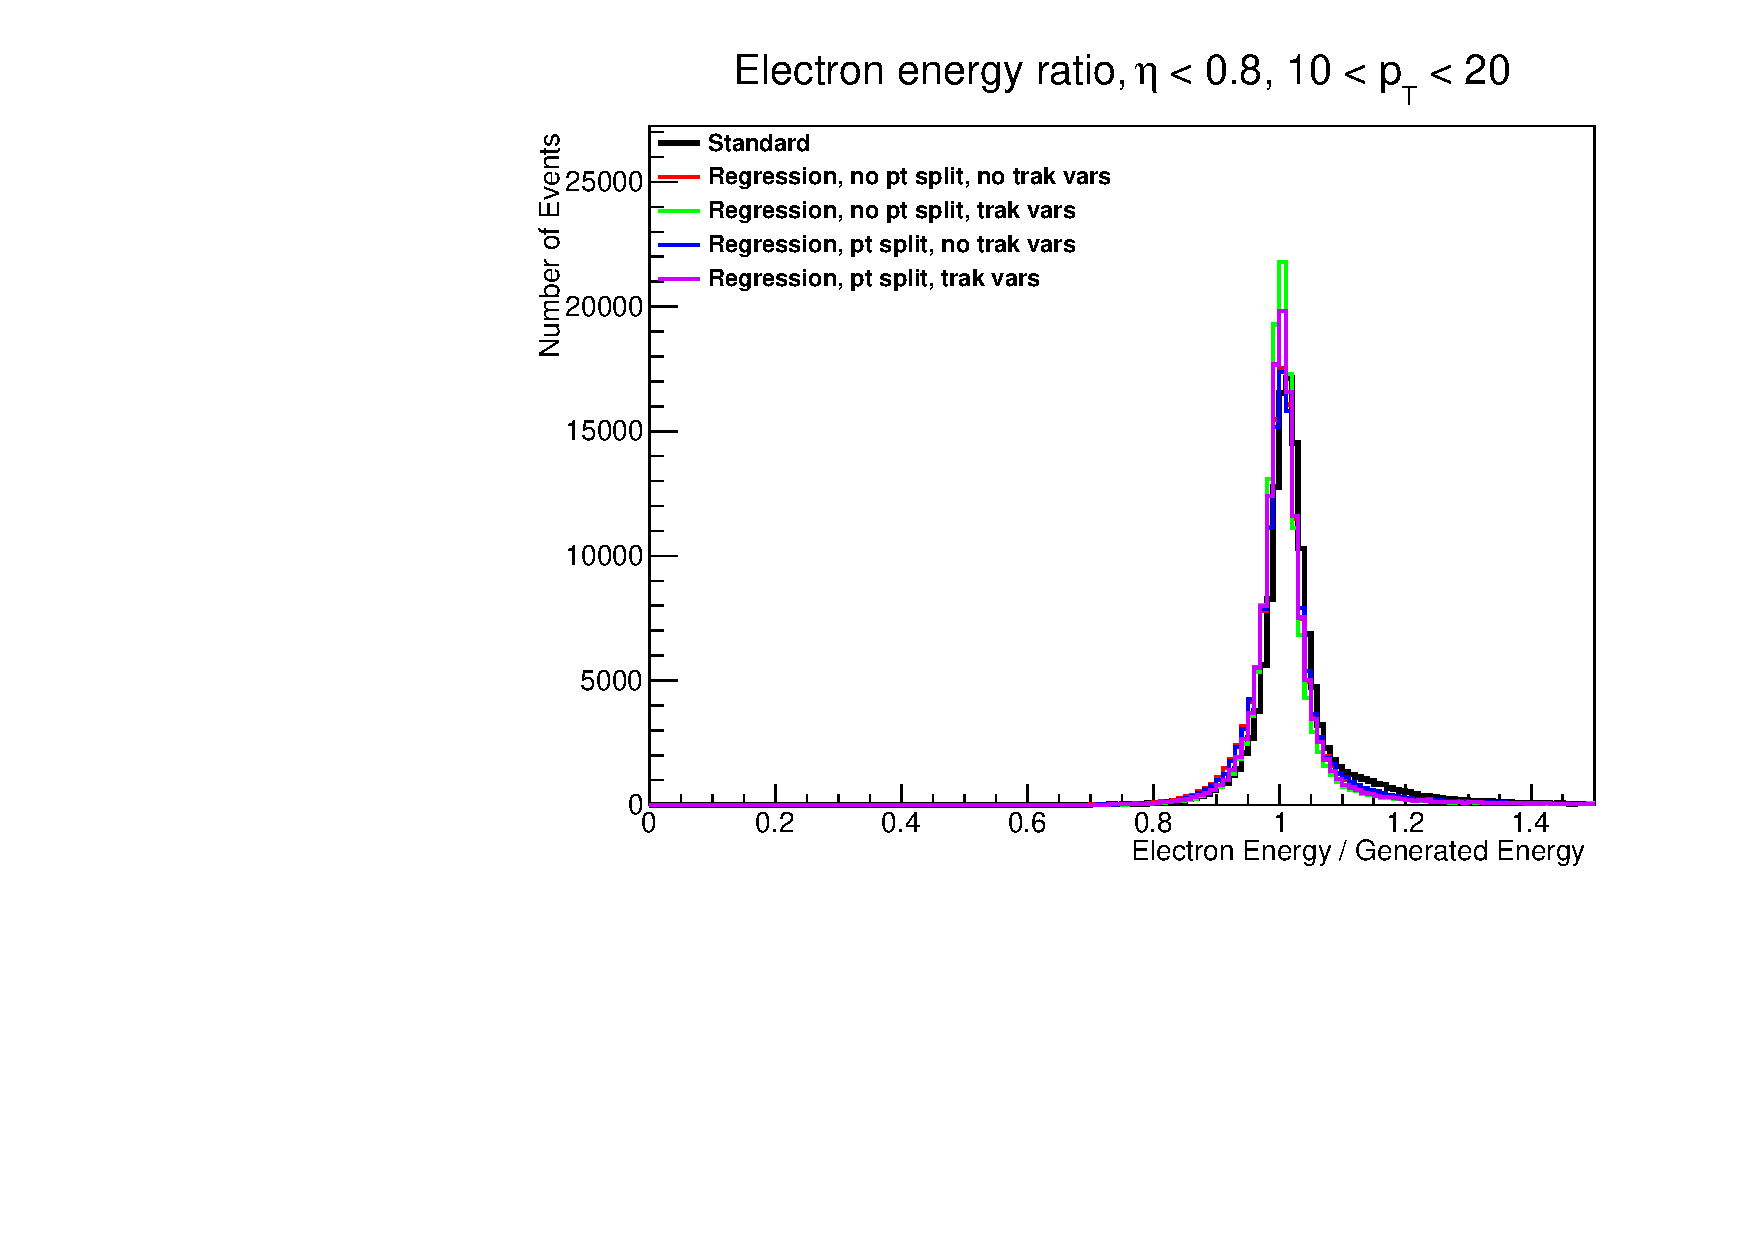
\includegraphics[width=0.6\textwidth]{figures/DY_cross_HZZ4l/EnergyResponse_allversions_binOption3.pdf}
	} \\
	\subfigure[]{
		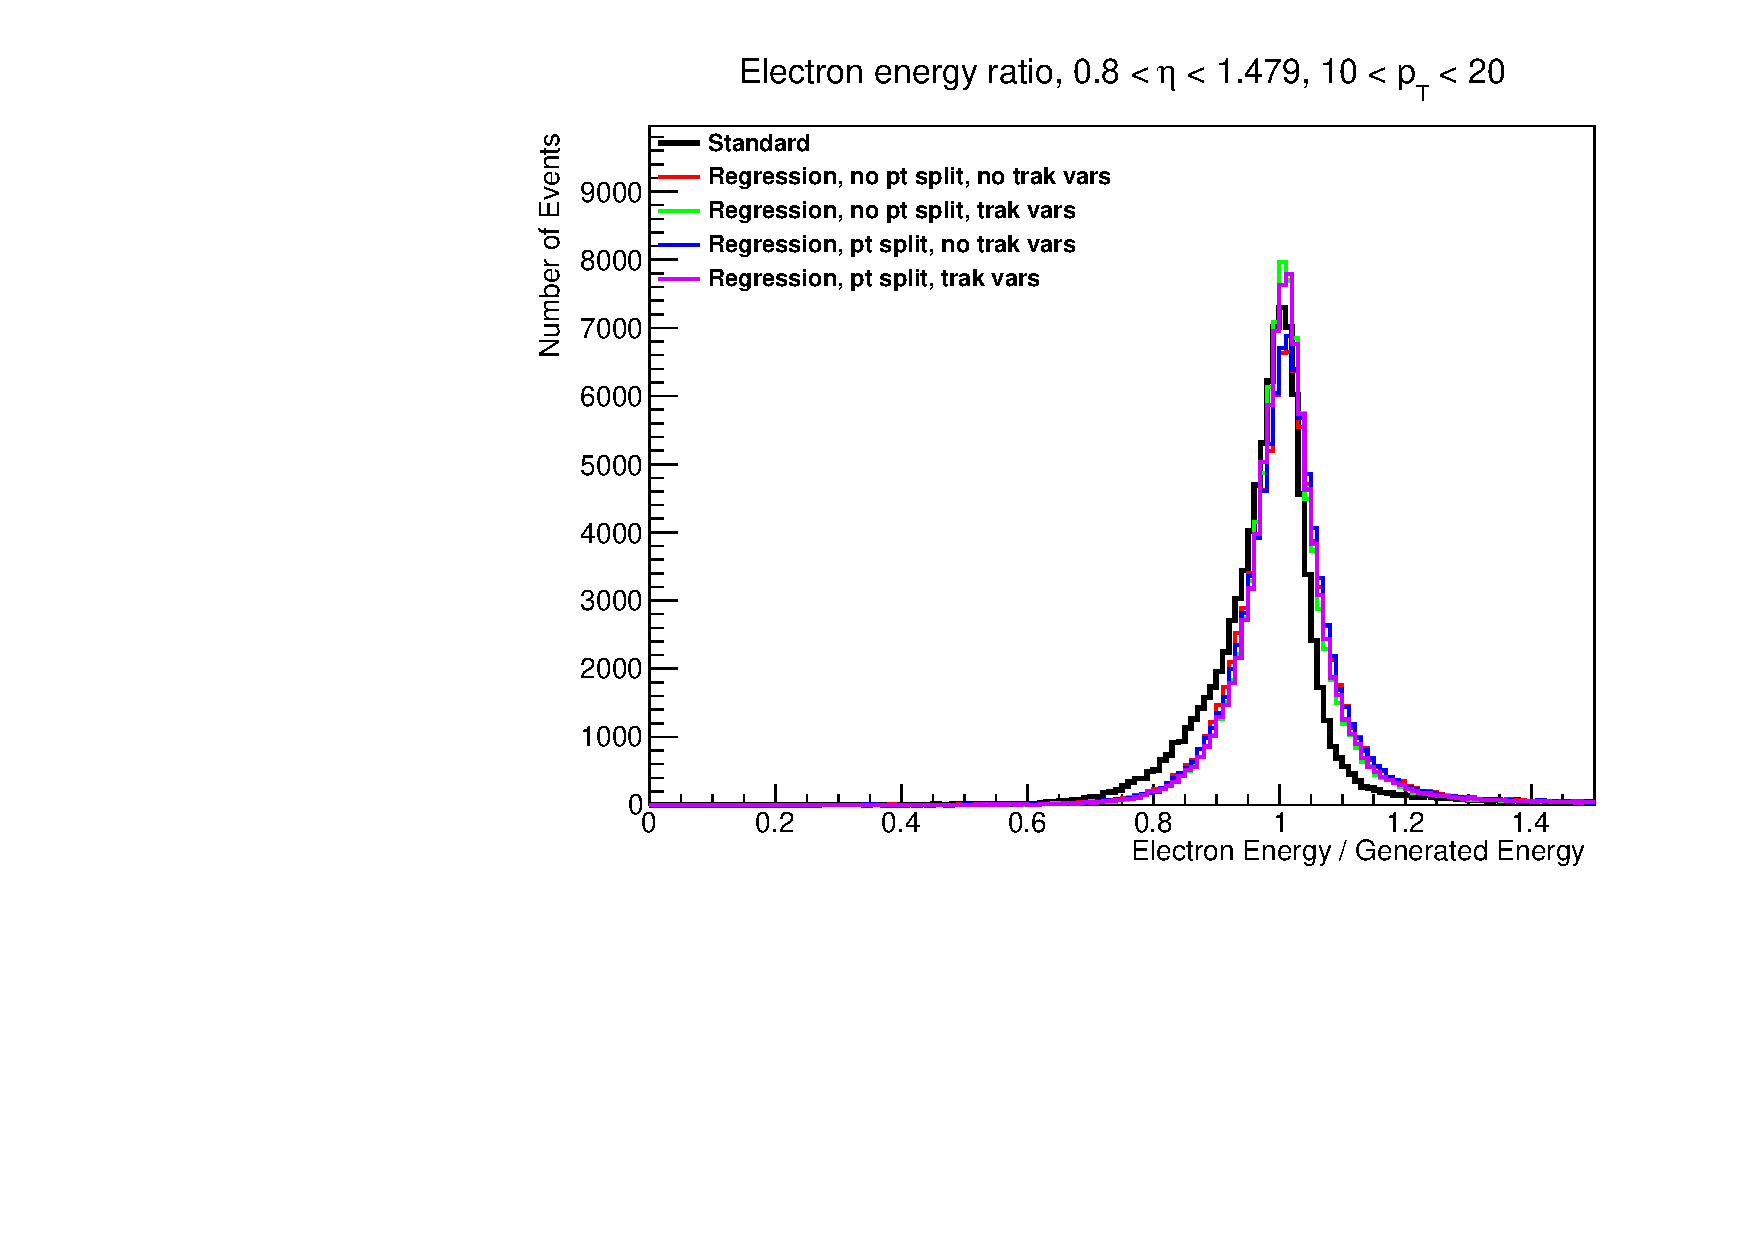
\includegraphics[width=0.6\textwidth]{figures/DY_cross_HZZ4l/EnergyResponse_allversions_binOption4.pdf}
	} \\
	\subfigure[]{
		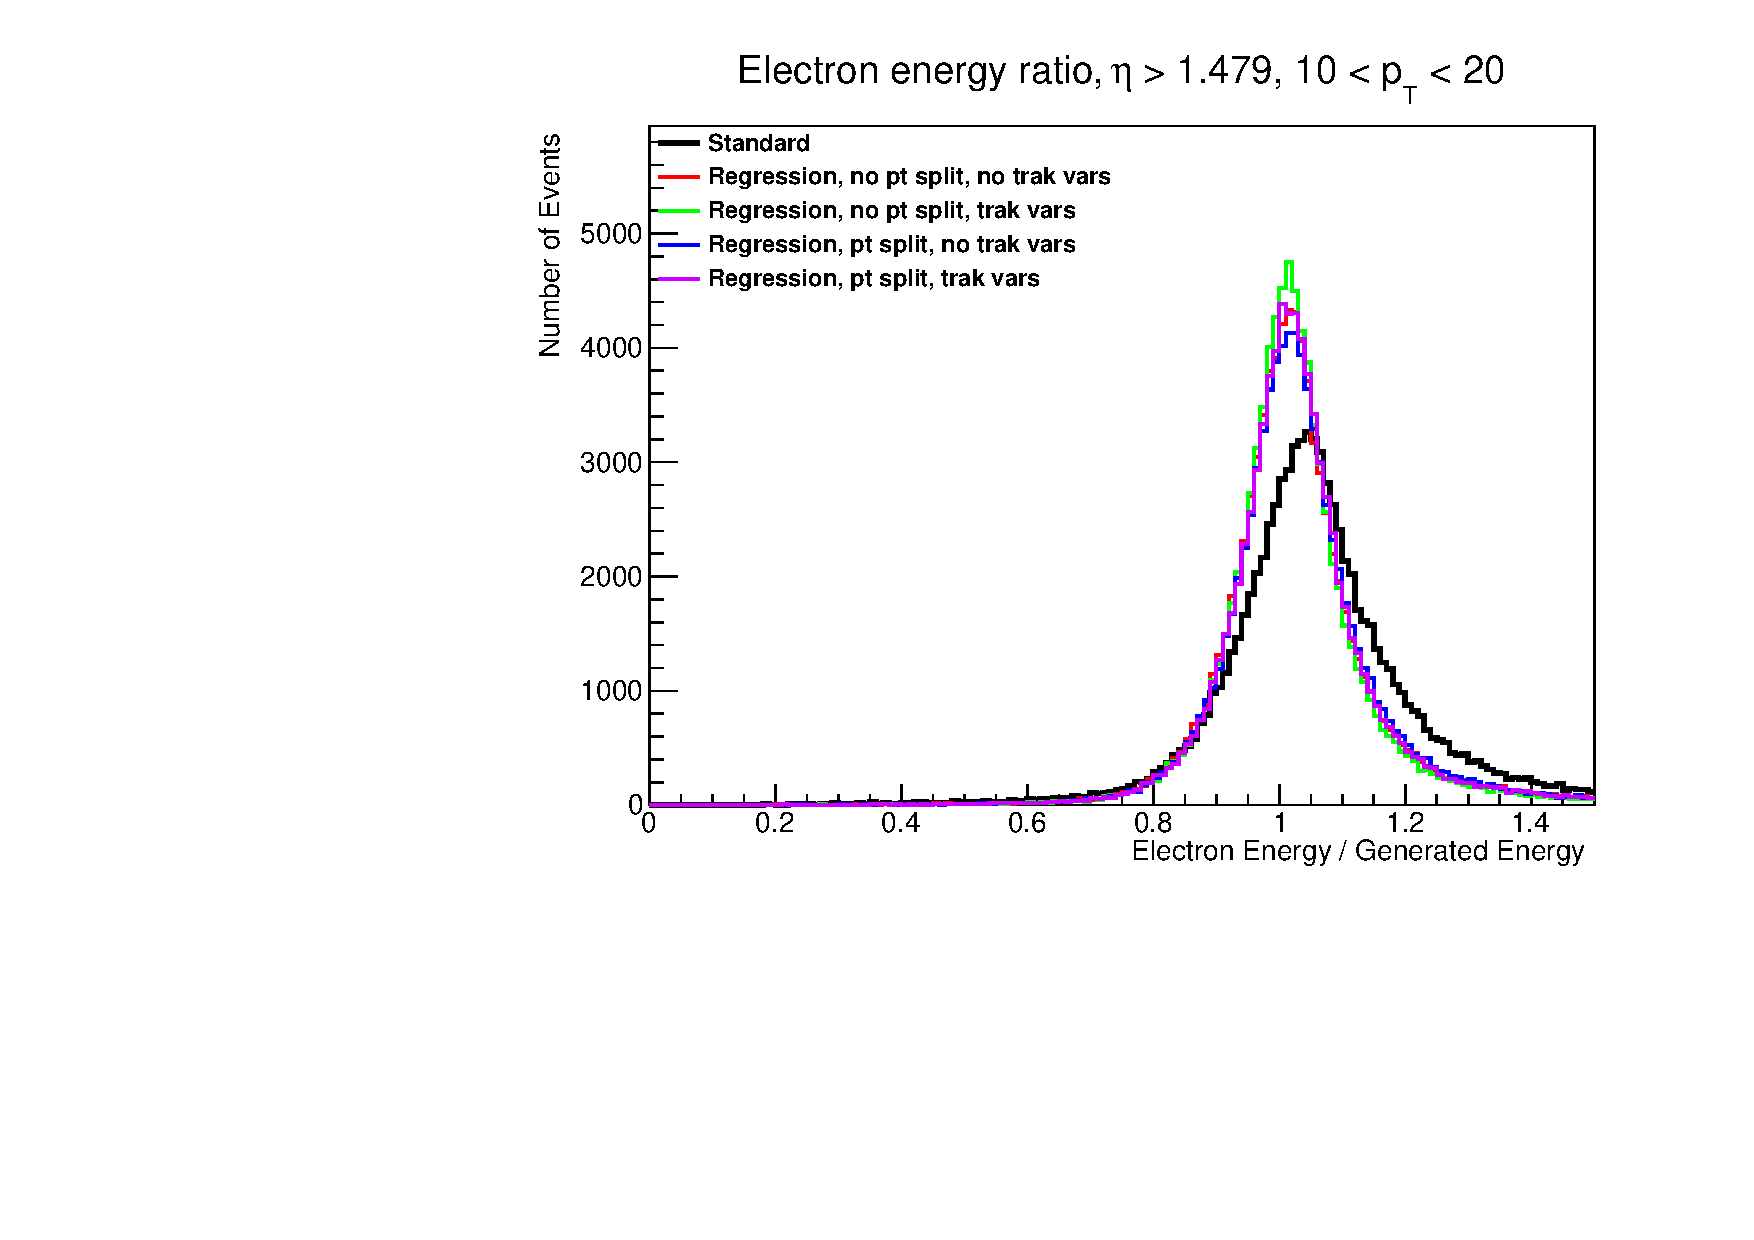
\includegraphics[width=0.6\textwidth]{figures/DY_cross_HZZ4l/EnergyResponse_allversions_binOption5.pdf}
	}
	\caption{Performance of regression trained on Drell-Yan and evaluated on Higgs Signal, medium $p_T$ bins}
	\label{fig:drellyanCrossHiggssignalEnergyResponse2}
\end{figure}

\begin{figure}[h]
\centering
	\subfigure[]{
		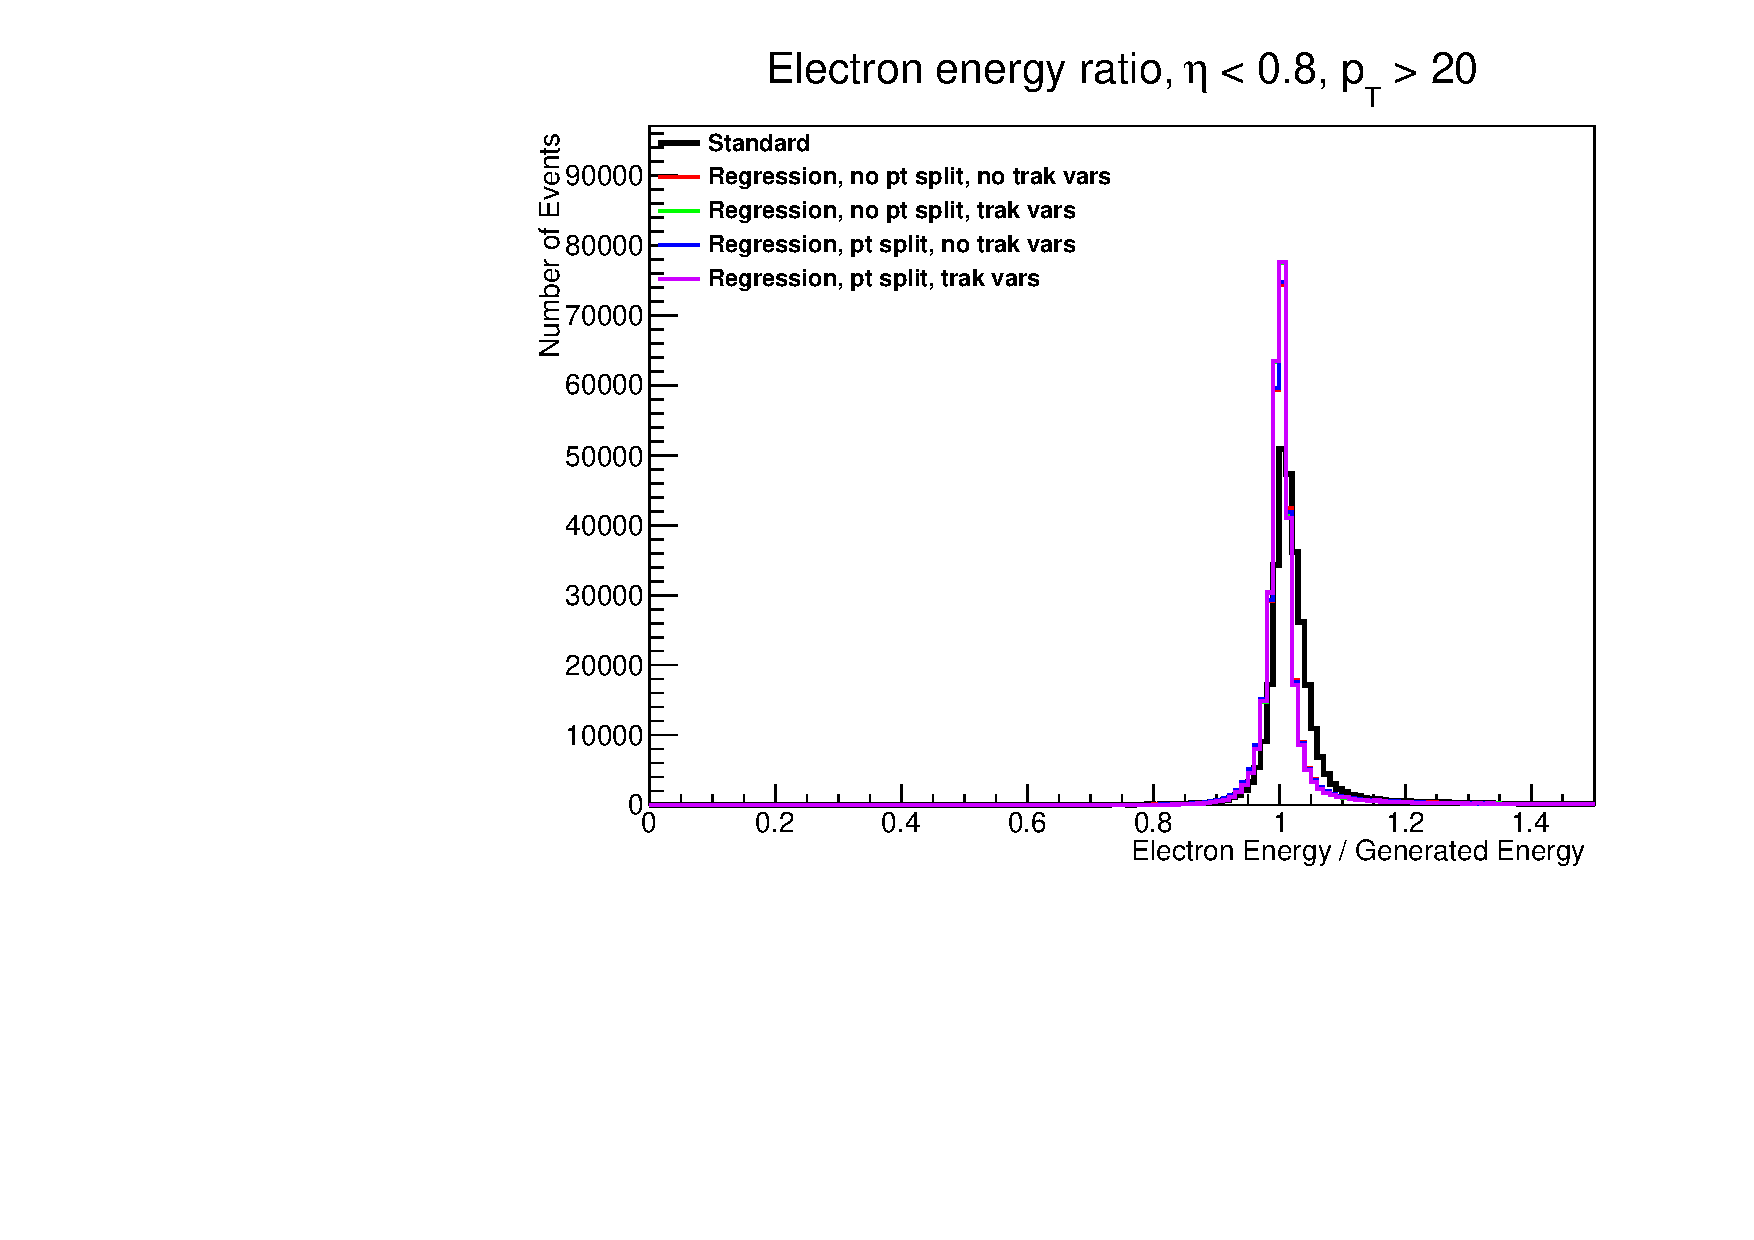
\includegraphics[width=0.6\textwidth]{figures/DY_cross_HZZ4l/EnergyResponse_allversions_binOption6.pdf}
	} \\
	\subfigure[]{
		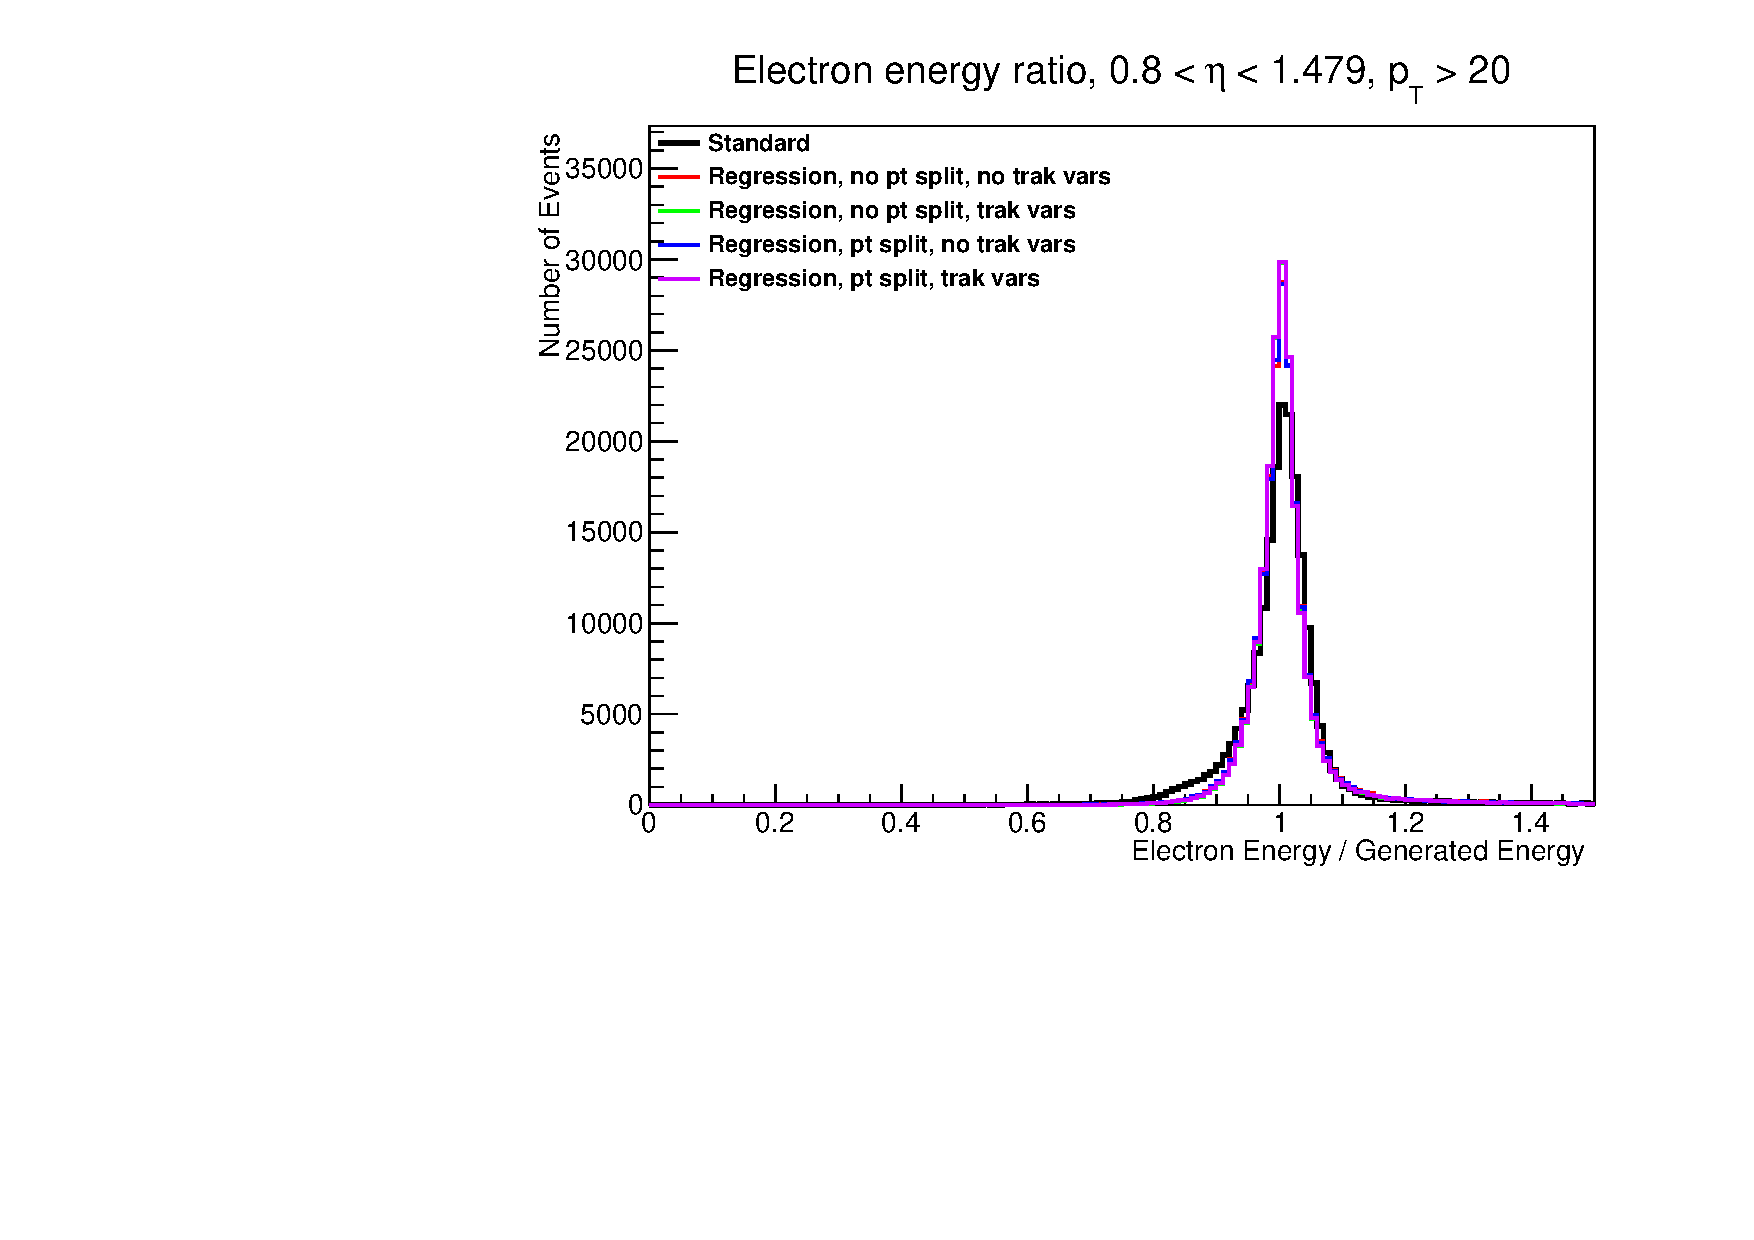
\includegraphics[width=0.6\textwidth]{figures/DY_cross_HZZ4l/EnergyResponse_allversions_binOption7.pdf}
	} \\
	\subfigure[]{
		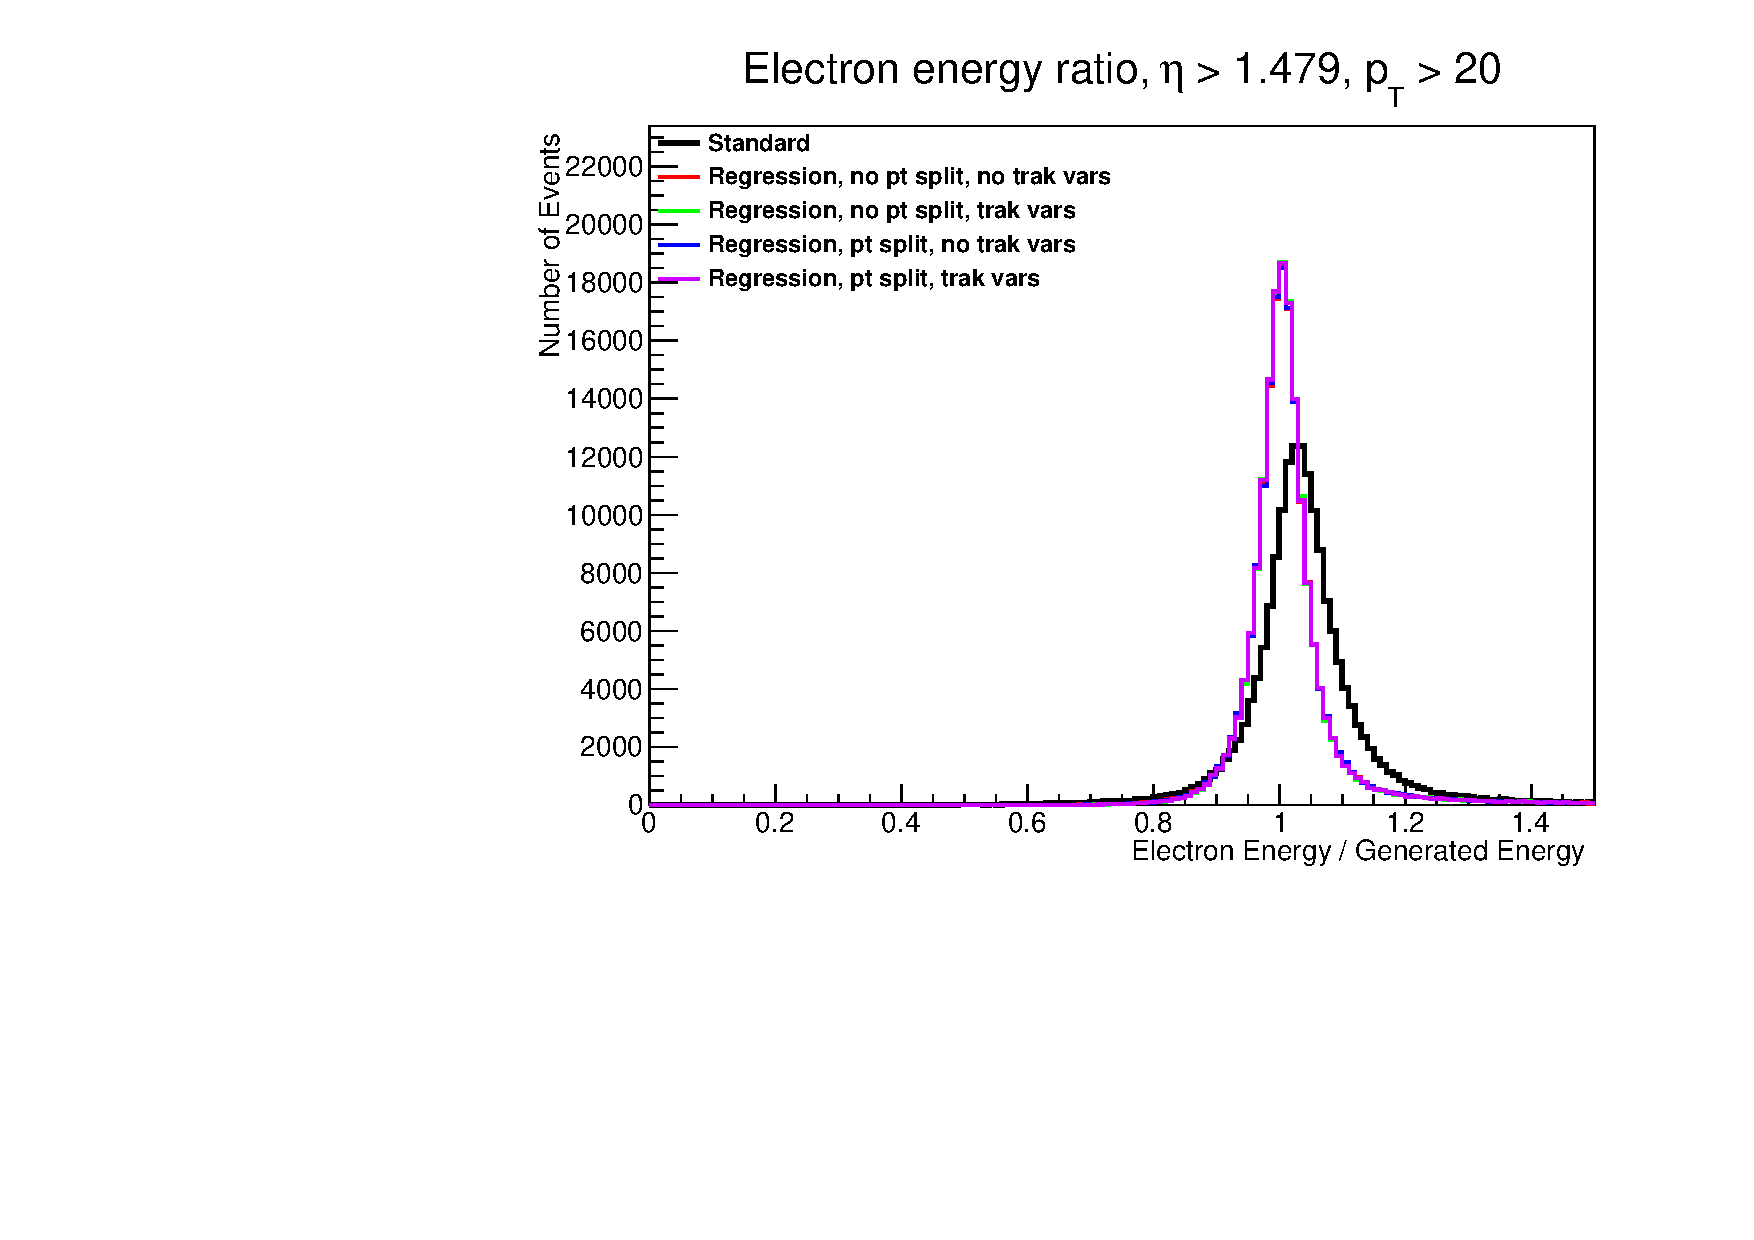
\includegraphics[width=0.6\textwidth]{figures/DY_cross_HZZ4l/EnergyResponse_allversions_binOption8.pdf}
	}
	\caption{Performance of regression trained on Drell-Yan and evaluated on Higgs Signal, high $p_T$ bins}
	\label{fig:drellyanCrossHiggssignalEnergyResponse3}
\end{figure}

\subsection{Performance Evaluated using \ZToEE\ mass spectrum} 
\label{subsec:zeesamplesperformance}

The resolution improvement brought by the electron energy regression is also evaluated in terms of its 
impact on the reconstructed Z mass spectrum. Using these samples also allow us to evaluate the difference 
in performance between data and Monte Carlo simulation. The samples used for the \ZToEE\ data and Monte Carlo
were given in Section \ref{sec:datasets}. For each sample, we compare the dielectron mass distribution for each regression 
with the mass computed using the standard electron momentum calculation.

(INSERT SOMETHING ABOUT CUTS ON ELECTRONS, LOW PT ETC.)

The distributions of the reconstructed Z masses can be seen for the MC sample in Figure \ref{fig:zmassMC} and for the data 
sample in Figure \ref{fig:zmassData}. We observe a significant improvement in mass resolution for the regression
compared to the standard momentum reconstruction. The different versions of the regression perform fairly similarly.

\begin{figure}[h]
	\centering
	\includegraphics[width=0.9 \textwidth]{figures/zmass/{ZeeNtuple.s12-zllm50-2-v9.Plots_zMass}.pdf}
	\caption{Distribution of reconstructed Z masses around Z pole, for the Monte Carlo sample}
	\label{fig:zmassMC}
\end{figure}

\begin{figure}[h]
	\centering 
	\includegraphics[width=0.9 \textwidth]{figures/zmass/{ZeeNtuple.2012Data.Plots_zMass}.pdf}
	\caption{Distribution of reconstructed Z masses around Z pole, for data}
	\label{fig:zmassData}
\end{figure}

\subsubsection{Energy Scale and Resolution Correction}
\label{sec:DataToMCCorrection}
Using the \ZToEE\ sample, we can determine any deviations in the average energy scale used to reconstruct
the momentum of the electrons in data, and any deviations between the average resolution 
predicted in the simulation and that observed in the data. We perform the same procedure used for the
\HiggsToGammaGamma\ analysis, where we perform a maximum likelihood fit to the dielectron mass distribution,
modelling the signal by the convolution of a Breit-Wigner function with a Crystal Ball function. The fit
is performed separately on data and Monte Carlo, where we extract the $\Delta$m and $\sigma$ parameters 
corresponding to the shift in the peak position of the \Z\ resonance and the width of the core of the 
mass resonance distribution. We extract these parameters in three bins of $|\eta|$, by performing 
the fit using events where both electron legs fall into the given $|\eta|$ bin. The resulting parameters
are summarized in Table \ref{tab:ScaleAndResolution_Standard} for the standard electron momentum
measurement and in Tables \ref{tab:ScaleAndResolution_Regression1} to \ref{tab:ScaleAndResolution_Regression4},
for the four versions of the regression. The fits from which the parameters are extracted are shown in 
Appendix \ref{sec:ScaleAndResolutionFits}. 



\begin{table}[!ht]
\begin{center} 
 Standard Electron Momentum Measurement \\
\begin{tabular}{|c|c|c|c|c|}
\hline
Bin   &   $\Delta m$ (MC)   &   $\Delta m$ (Data)  &  $\sigma$ (MC)  &   $\sigma$ (Data)  \\  \hline
$0.0 \le |\eta| < 1.0$ & $1.055 \pm 0.006$ & $0.388 \pm 0.005$ & $1.546 \pm 0.006$ & $1.592 \pm 0.006$ \\\hline
$1.0 \le |\eta| < 1.479$ & $-0.222 \pm 0.016$ & $-1.627 \pm 0.019$ & $2.598 \pm 0.017$ & $3.021 \pm 0.019$ \\\hline
$1.479 \le |\eta| < 2.5$ & $2.227 \pm 0.012$ & $0.261 \pm 0.015$ & $3.166 \pm 0.013$ & $4.210 \pm 0.015$ \\\hline
\end{tabular}
\caption{The parameters for the mass shift and the width of the crystal ball resolution function are 
shown for the data and Monte Carlo simulation in different bins of electron $\eta$ for the standard
electron momentum measurement. }
\label{tab:ScaleAndResolution_Standard}
\end{center}
\end{table}



\begin{table}[!ht]
\begin{center} 
 Regression without track-related variables and without $p_{T}$ bin splitting \\
\begin{tabular}{|c|c|c|c|c|}
\hline
Bin   &   $\Delta m$ (MC)   &   $\Delta m$ (Data)  &  $\sigma$ (MC)  &   $\sigma$ (Data)  \\  \hline
$0.0 \le |\eta| < 1.0$ & $0.027 \pm 0.005$ & $0.046 \pm 0.004$ & $1.049 \pm 0.006$ & $1.239 \pm 0.005$ \\\hline
$1.0 \le |\eta| < 1.479$ & $-0.265 \pm 0.018$ & $-1.093 \pm 0.016$ & $2.135 \pm 0.019$ & $2.539 \pm 0.017$ \\\hline
$1.479 \le |\eta| < 2.5$ & $-0.199 \pm 0.010$ & $-0.836 \pm 0.013$ & $1.906 \pm 0.011$ & $3.680 \pm 0.014$ \\\hline




\end{tabular}
\caption{ The parameters for the mass shift and the width of the crystal ball resolution function are 
shown for the data and Monte Carlo simulation in different bins of electron $\eta$ for the regression
trained without track-related variables and no $p_{T}$ bin splitting.}
\label{tab:ScaleAndResolution_Regression1}
\end{center}
\end{table}

\begin{table}[!ht]
\begin{center} 
 Regression with track-related variables and without $p_{T}$ bin splitting \\
\begin{tabular}{|c|c|c|c|c|}
\hline
Bin   &   $\Delta m$ (MC)   &   $\Delta m$ (Data)  &  $\sigma$ (MC)  &   $\sigma$ (Data)  \\  \hline
$0.0 \le |\eta| < 1.0$ & $0.031 \pm 0.005$ & $0.048 \pm 0.004$ & $1.050 \pm 0.006$ & $1.239 \pm 0.005$ \\\hline
$1.0 \le |\eta| < 1.479$ & $-0.274 \pm 0.018$ & $-0.951 \pm 0.016$ & $2.154 \pm 0.019$ & $2.421 \pm 0.015$ \\\hline
$1.479 \le |\eta| < 2.5$ & $-0.198 \pm 0.010$ & $-0.827 \pm 0.013$ & $1.906 \pm 0.011$ & $3.678 \pm 0.014$ \\\hline
\end{tabular}
\caption{The parameters for the mass shift and the width of the crystal ball resolution function are 
shown for the data and Monte Carlo simulation in different bins of electron $\eta$ for the regression
trained with track-related variables and no $p_{T}$ bin splitting.}
\label{tab:ScaleAndResolution_Regression2}
\end{center}
\end{table}


\begin{table}[!ht]
\begin{center} 
 Regression without track-related variables and with $p_{T}$ bin splitting \\
\begin{tabular}{|c|c|c|c|c|}
\hline
Bin   &   $\Delta m$ (MC)   &   $\Delta m$ (Data)  &  $\sigma$ (MC)  &   $\sigma$ (Data)  \\  \hline
$0.0 \le |\eta| < 1.0$ & $0.054 \pm 0.005$ & $0.117 \pm 0.004$ & $1.099 \pm 0.006$ & $1.297 \pm 0.005$ \\\hline
$1.0 \le |\eta| < 1.479$ & $-0.263 \pm 0.017$ & $-1.188 \pm 0.016$ & $2.244 \pm 0.018$ & $2.652 \pm 0.017$ \\\hline
$1.479 \le |\eta| < 2.5$ & $-0.189 \pm 0.010$ & $-0.854 \pm 0.014$ & $1.931 \pm 0.011$ & $3.739 \pm 0.014$ \\\hline
\end{tabular}
\caption{The parameters for the mass shift and the width of the crystal ball resolution function are 
shown for the data and Monte Carlo simulation in different bins of electron $\eta$ for the regression
trained without track-related variables and with $p_{T}$ bin splitting.}
\label{tab:ScaleAndResolution_Regression3}
\end{center}
\end{table}

\clearpage

\begin{table}[!ht]
\begin{center} 
 Regression with track-related variables and with $p_{T}$ bin splitting \\
\begin{tabular}{|c|c|c|c|c|}
\hline
Bin   &   $\Delta m$ (MC)   &   $\Delta m$ (Data)  &  $\sigma$ (MC)  &   $\sigma$ (Data)  \\  \hline
$0.0 \le |\eta| < 1.0$ & $0.060 \pm 0.005$ & $0.122 \pm 0.004$ & $1.095 \pm 0.006$ & $1.294 \pm 0.005$ \\\hline
$1.0 \le |\eta| < 1.479$ & $-0.257 \pm 0.018$ & $-1.175 \pm 0.016$ & $2.247 \pm 0.019$ & $2.663 \pm 0.017$ \\\hline
$1.479 \le |\eta| < 2.5$ & $-0.182 \pm 0.010$ & $-0.841 \pm 0.014$ & $1.928 \pm 0.011$ & $3.741 \pm 0.014$ \\\hline
\end{tabular}
\caption{The parameters for the mass shift and the width of the crystal ball resolution function are 
shown for the data and Monte Carlo simulation in different bins of electron $\eta$ for the regression
trained with track-related variables and with $p_{T}$ bin splitting.}
\label{tab:ScaleAndResolution_Regression4} 
\end{center}
\end{table}


From these parameters we determine energy corrections to be applied to the data electrons, described by:

\begin{eqnarray}
  \label{eqn:DeltaE} 
\frac{\Delta E}{E} = \frac{\Delta m_{\mathrm{Data}} - \Delta m_{\mathrm{MC}}}{m_{\mathrm{Z}} + \Delta m_{\mathrm{MC}}},
\end{eqnarray} 

where $\frac{\Delta E}{e}$ is the size of the energy scale correction expressed as a fraction of the 
energy of the electron, and terms that are second order in $\frac{\Delta E}{E}$ are neglected. 
The additional gaussian smearing that must be applied to the energy of each electron in the
Monte Carlo simulation is determined by subtracting in quadrature the width parameter obtained from the fit to the
simulation from the width parameter obtained from the data fit. The expression is given by:

\begin{eqnarray}
  \label{eqn:DeltaE} 
\frac{\sigma_{E}}{E} = \sqrt{2}\times\frac{\sigma^{\mathrm{CB}}_{\mathrm{Data}} - \sigma^{\mathrm{CB}}_{\mathrm{MC}}}{\times(m_{\mathrm{Z}} + \Delta m_{\mathrm{MC}})},
\end{eqnarray} 
 
where $\frac{\sigma_{E}}{E}$ is the width of the gaussian with which we smear the energy of the electrons
in the Monte Carlo simulation expressed as a fraction of the electron energy, and
$\sigma^{\mathrm{CB}}$ is the width parameter of the fitted Crystal Ball function. The energy scale
correction parameters and width parameters for the extra smearing are 
summarized in Tables \ref{tab:EnergyScaleAndResolutionCorrection_Regression1} to \ref{tab:EnergyScaleAndResolutionCorrection_Regression4}
for the four versions of the regressions.


\begin{table}[!ht]
\begin{center} 
 Regression without trk var \\
\begin{tabular}{|c|c|c|}
\hline
Bin   &   $\Delta E/E$ &   $\sigma_{E}/E$ \\  \hline
$0.0 \le |\eta| < 1.0$ & $0.00020 \pm 0.00007$ & $0.0102 \pm 0.0002$ \\\hline
$1.0 \le |\eta| < 1.479$ & $-0.0091 \pm 0.0003$ & $0.0214 \pm 0.0007$ \\\hline
$1.479 \le |\eta| < 2.5$ & $-0.0070 \pm 0.0002$ & $0.0489 \pm 0.0003$ \\\hline
\end{tabular}
\caption{The energy scale correction and the width of the additional gaussian smearing function
expressed as a fraction of the electron energy 
are shown for different bins of electron $\eta$ for the regression trained 
without track-related variables and without $p_{T}$ bin splitting. }
\label{tab:EnergyScaleAndResolutionCorrection_Regression1}
\end{center}
\end{table}


\begin{table}[!ht]
\begin{center} 
 Regression with trk var \\
\begin{tabular}{|c|c|c|}
\hline
Bin   &   $\Delta E/E$ &   $\sigma_{E}/E$ \\  \hline
$0.0 \le |\eta| < 1.0$ & $0.00019 \pm 0.00007$ & $0.0102 \pm 0.0002$ \\\hline
$1.0 \le |\eta| < 1.479$ & $-0.0074 \pm 0.0003$ & $0.0172 \pm 0.0008$ \\\hline
$1.479 \le |\eta| < 2.5$ & $-0.0069 \pm 0.0002$ & $0.0489 \pm 0.0003$ \\\hline
\end{tabular}
\caption{The energy scale correction and the width of the additional gaussian smearing function
expressed as a fraction of the electron energy 
are shown for different bins of electron $\eta$ for the regression trained 
with track-related variables and without $p_{T}$ bin splitting.}
\label{tab:EnergyScaleAndResolutionCorrection_Regression2}
\end{center}
\end{table}

 
\begin{table}[!ht]
\begin{center} 
 Regression without trk var, two pt bins \\
\begin{tabular}{|c|c|c|}
\hline
Bin   &   $\Delta E/E$ &   $\sigma_{E}/E$ \\  \hline
$0.0 \le |\eta| < 1.0$ & $0.00069 \pm 0.00007$ & $0.0107 \pm 0.0002$ \\\hline
$1.0 \le |\eta| < 1.479$ & $-0.0102 \pm 0.0003$ & $0.0220 \pm 0.0007$ \\\hline
$1.479 \le |\eta| < 2.5$ & $-0.0073 \pm 0.0002$ & $0.0498 \pm 0.0003$ \\\hline
\end{tabular}
\caption{The energy scale correction and the width of the additional gaussian smearing function
expressed as a fraction of the electron energy 
are shown for different bins of electron $\eta$ for the regression trained 
without track-related variables and with $p_{T}$ bin splitting.}
\label{tab:EnergyScaleAndResolutionCorrection_Regression3}
\end{center}
\end{table}


\begin{table}[!ht]
\begin{center} 
 Regression with trk var, two pt bins \\
\begin{tabular}{|c|c|c|}
\hline
Bin   &   $\Delta E/E$ &   $\sigma_{E}/E$ \\  \hline
$0.0 \le |\eta| < 1.0$ & $0.00068 \pm 0.00007$ & $0.0107 \pm 0.0002$ \\\hline
$1.0 \le |\eta| < 1.479$ & $-0.0101 \pm 0.0003$ & $0.0222 \pm 0.0007$ \\\hline
$1.479 \le |\eta| < 2.5$ & $-0.0072 \pm 0.0002$ & $0.0498 \pm 0.0003$ \\\hline
\end{tabular}
\caption{The energy scale correction and the width of the additional gaussian smearing function
expressed as a fraction of the electron energy 
are shown for different bins of electron $\eta$ for the regression trained 
with track-related variables and with $p_{T}$ bin splitting.} 
\label{tab:EnergyScaleAndResolutionCorrection_Regression4}
\end{center}
\end{table}


The impact of these energy scale and resolution corrections are illustrated by comparing Figure~\ref{fig:ZMassValidation_BeforeCorr}
with Figure~\ref{fig:ZMassValidation_AfterCorr}, where we plot the reconstructed Z mass distributions for \ZToEE\ events
before and after the corrections in different kinematic bins. The regression trained with track-related variables and 
without $p_{T}$ bin splitting is used for these plots. The agreement between data and Monte Carlo simulation is
significantly improved after the corrections. Small residual discrepancies remain even after the corrections, which are 
propagated as systematic uncertainties. 
 
\clearpage

\begin{figure}[h]
\centering
  \subfigure[Central Barrel, Central Barrel]{
    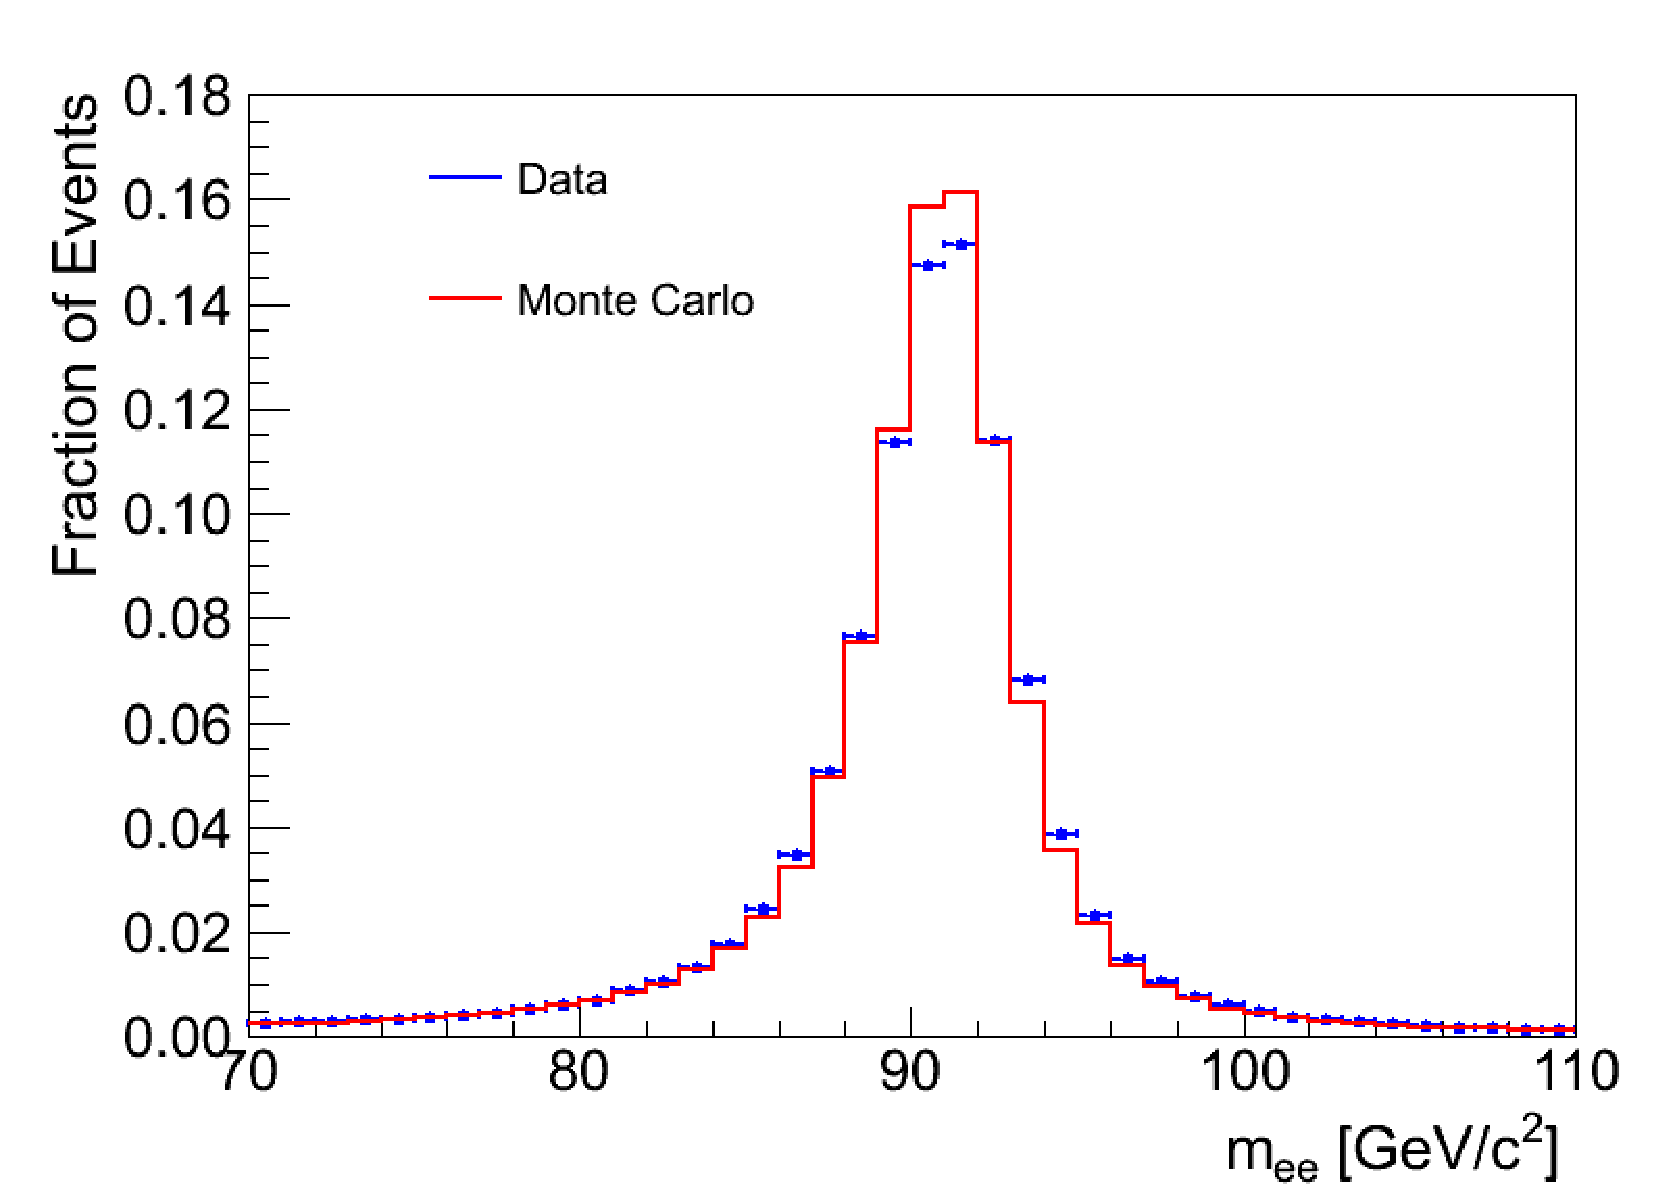
\includegraphics[width=0.45\textwidth]{figures/ZeeMassScaleAndResolutionValidationPlots_EnergyType2_BeforeCorr_CategoryBin0.pdf}
  } 
  \subfigure[Central Barrel, Outer Barrel ]{
    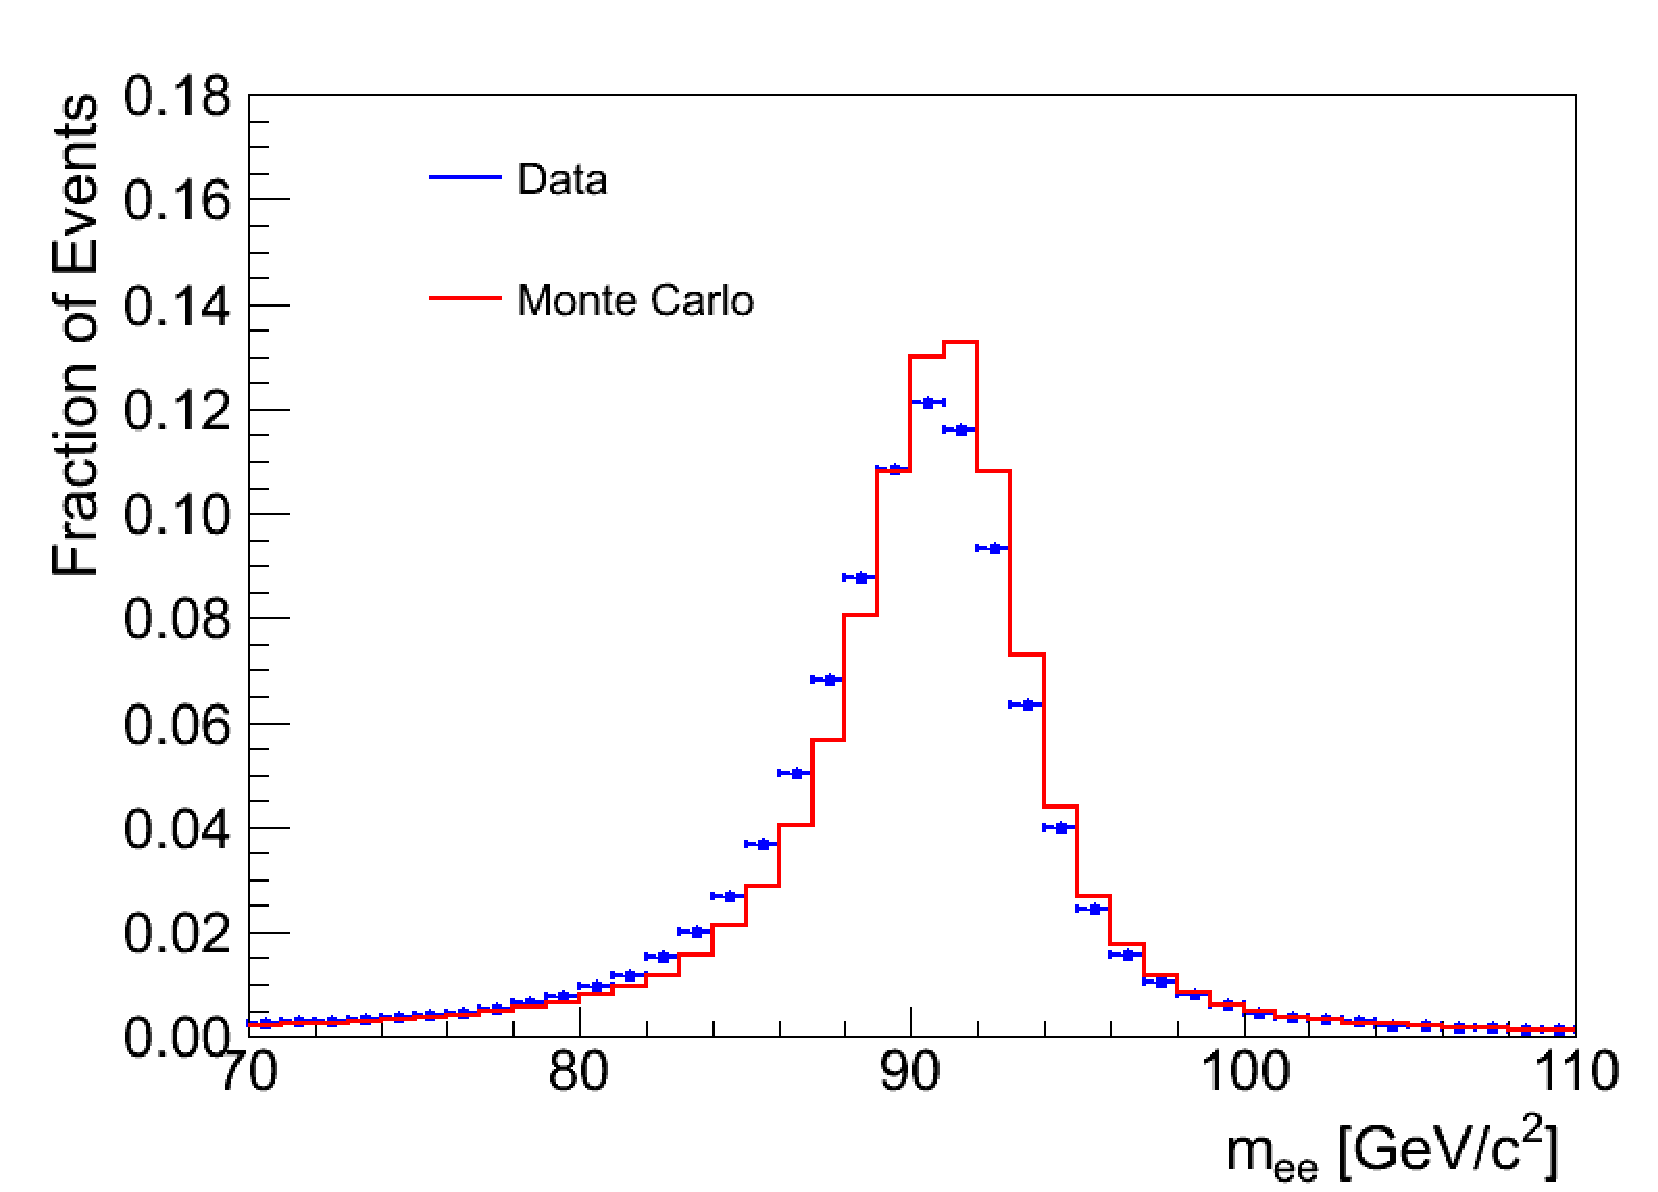
\includegraphics[width=0.45\textwidth]{figures/ZeeMassScaleAndResolutionValidationPlots_EnergyType2_BeforeCorr_CategoryBin1.pdf}
  } 
  \subfigure[Central Barrel, Endcap ]{
    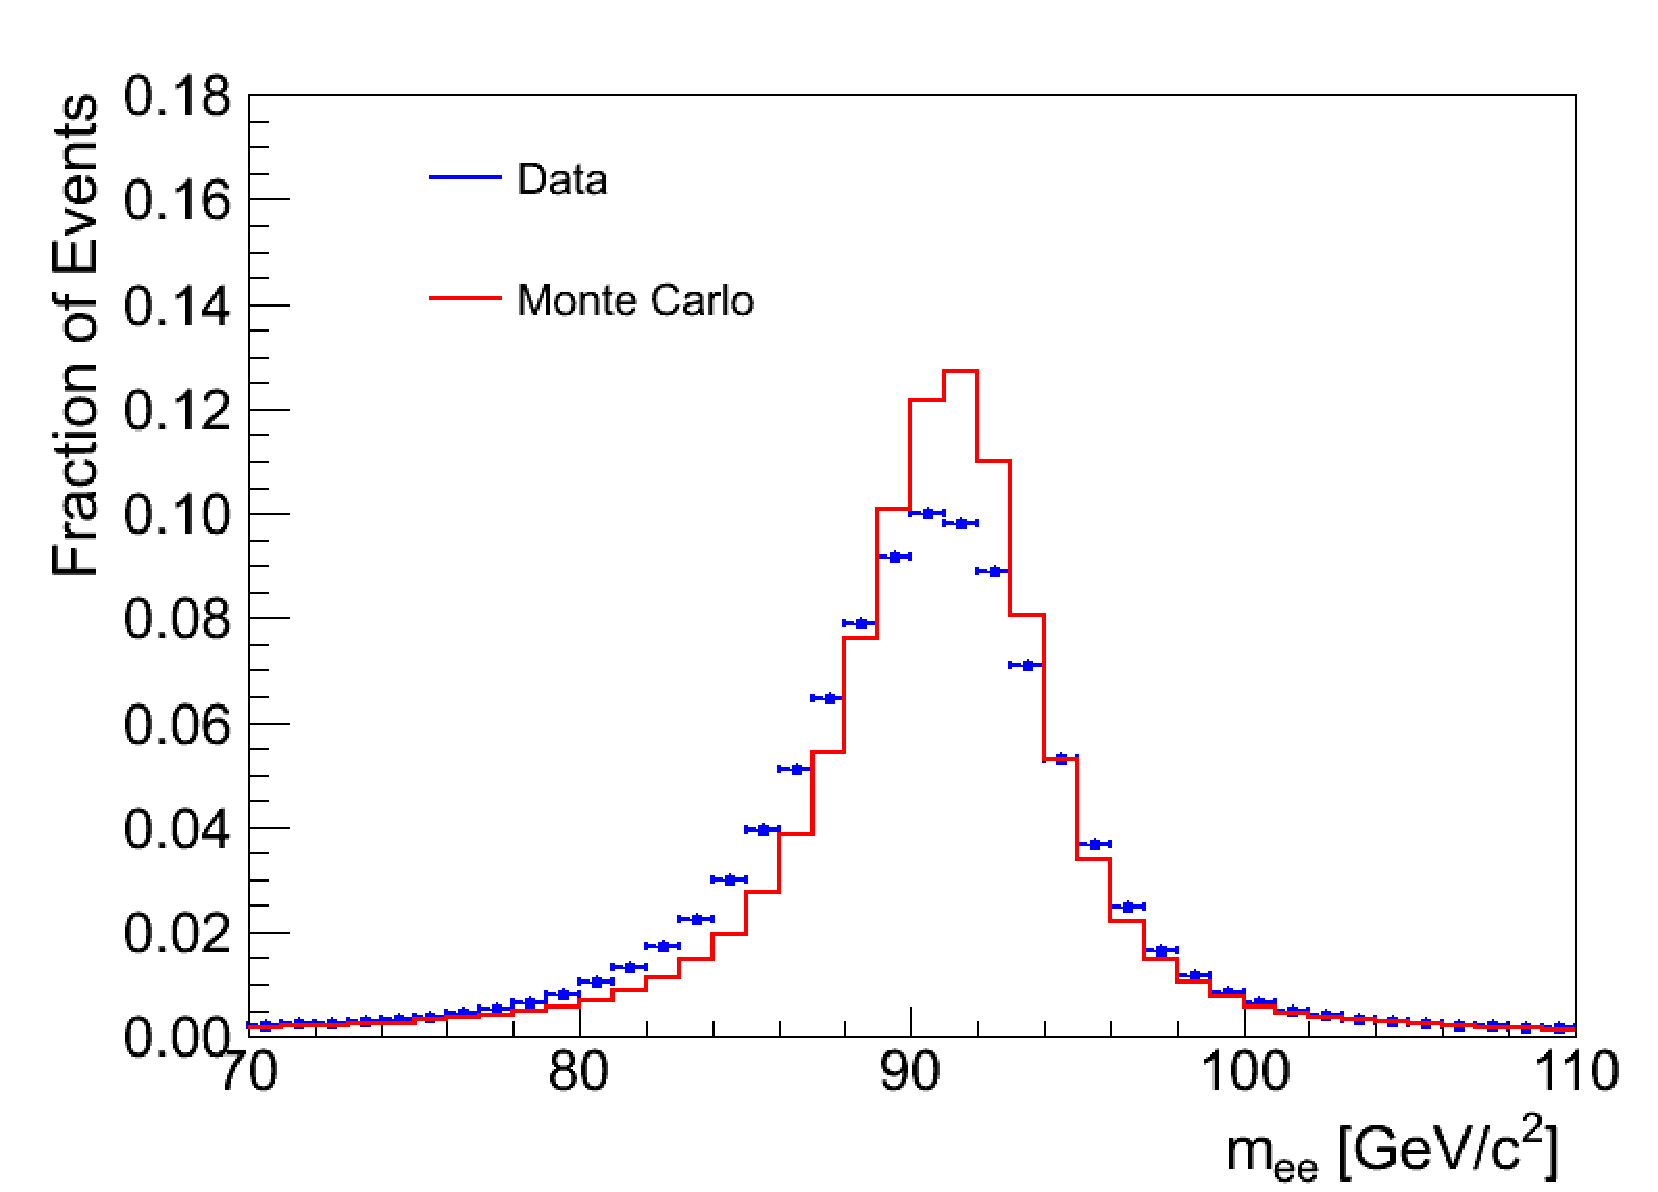
\includegraphics[width=0.45\textwidth]{figures/ZeeMassScaleAndResolutionValidationPlots_EnergyType2_BeforeCorr_CategoryBin2.pdf}
  } 
  \subfigure[Outer Barrel, Outer Barrel ]{
    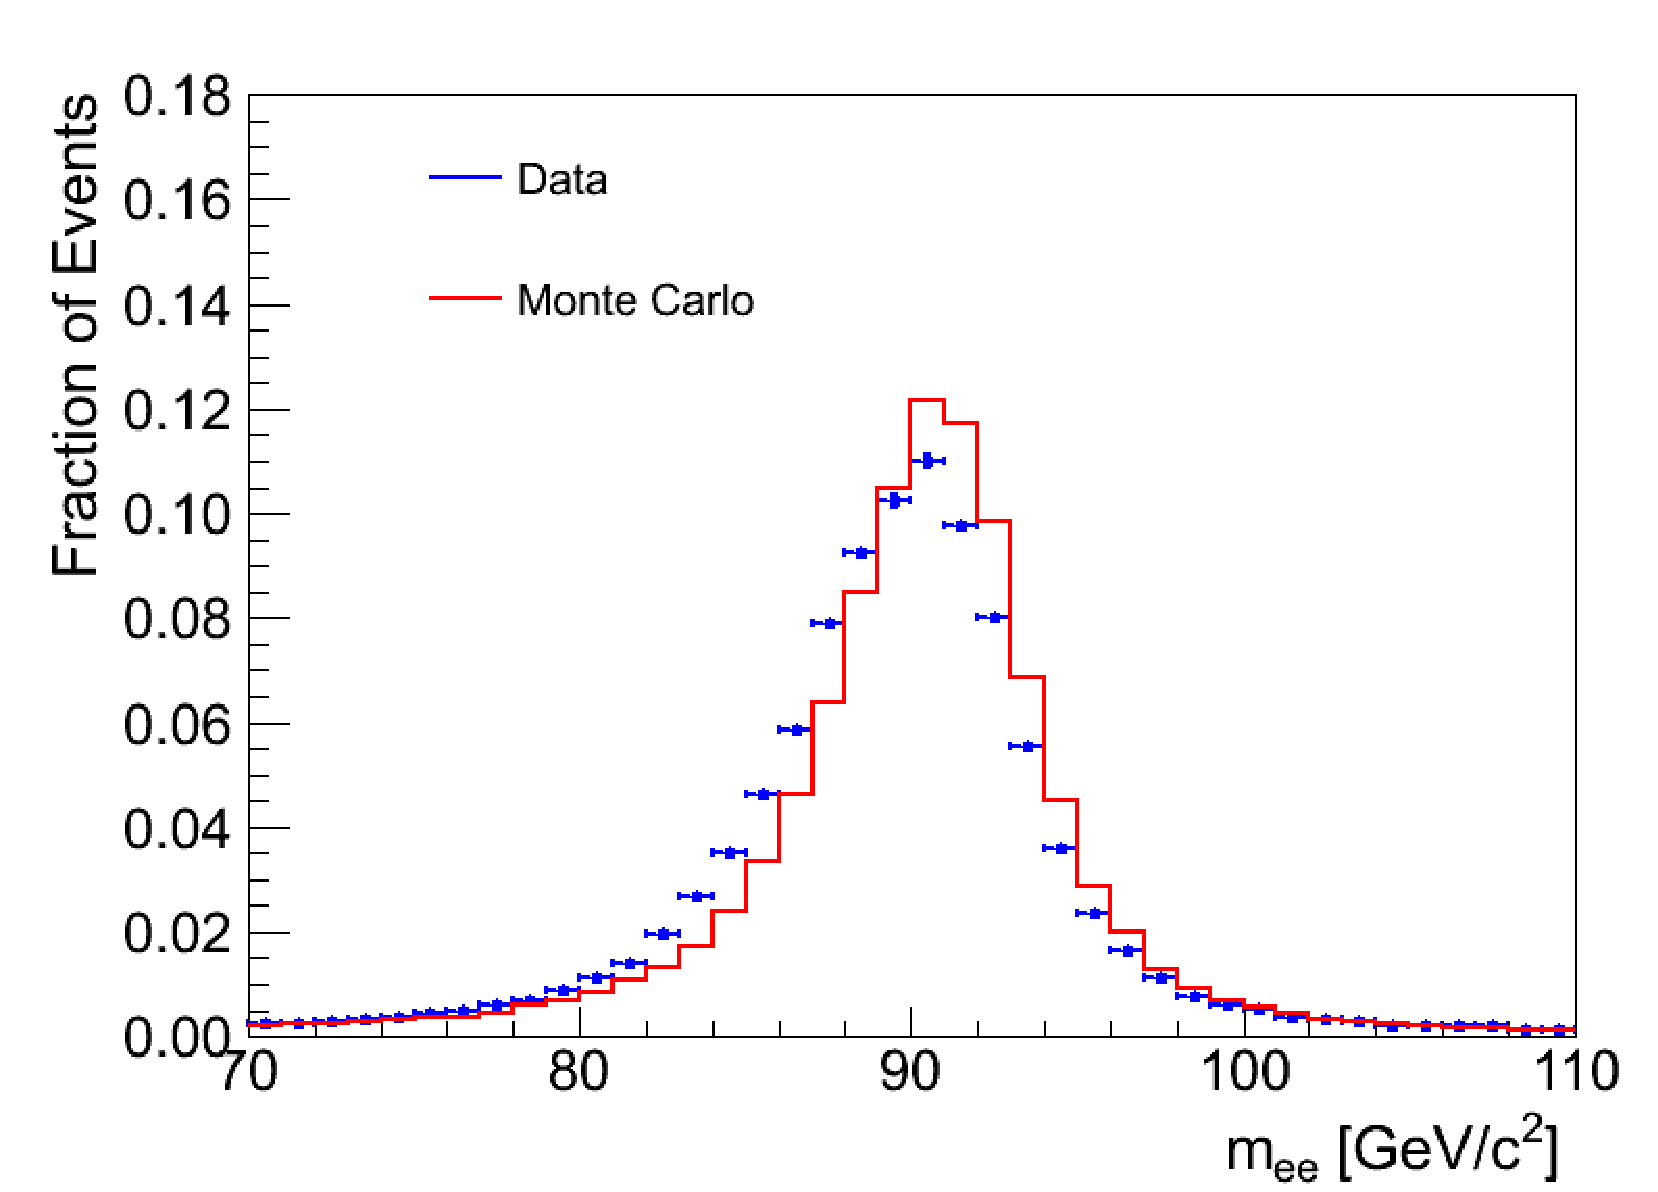
\includegraphics[width=0.45\textwidth]{figures/ZeeMassScaleAndResolutionValidationPlots_EnergyType2_BeforeCorr_CategoryBin3.pdf}
  } 
  \subfigure[Outer Barrel, Endcap Barrel]{
    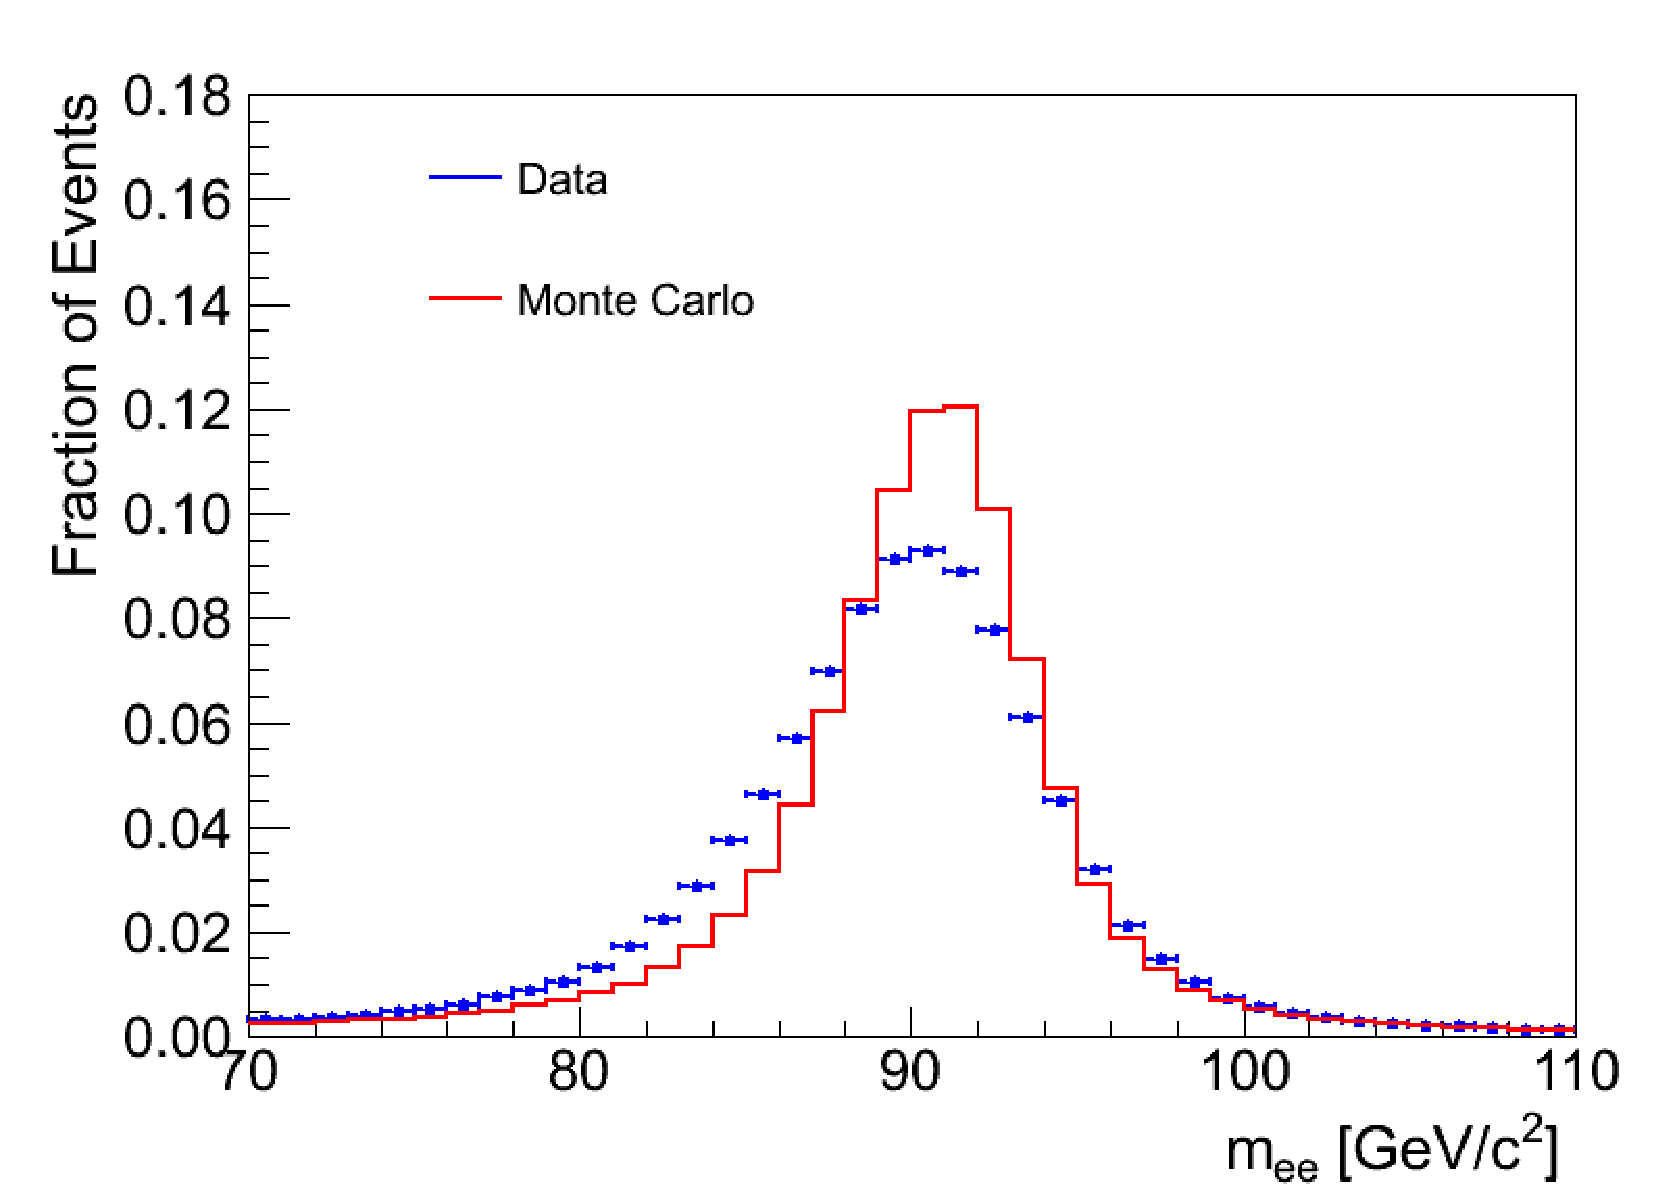
\includegraphics[width=0.45\textwidth]{figures/ZeeMassScaleAndResolutionValidationPlots_EnergyType2_BeforeCorr_CategoryBin4.pdf}
  } 
  \subfigure[Endcap Barrel, Endcap Barrel]{
    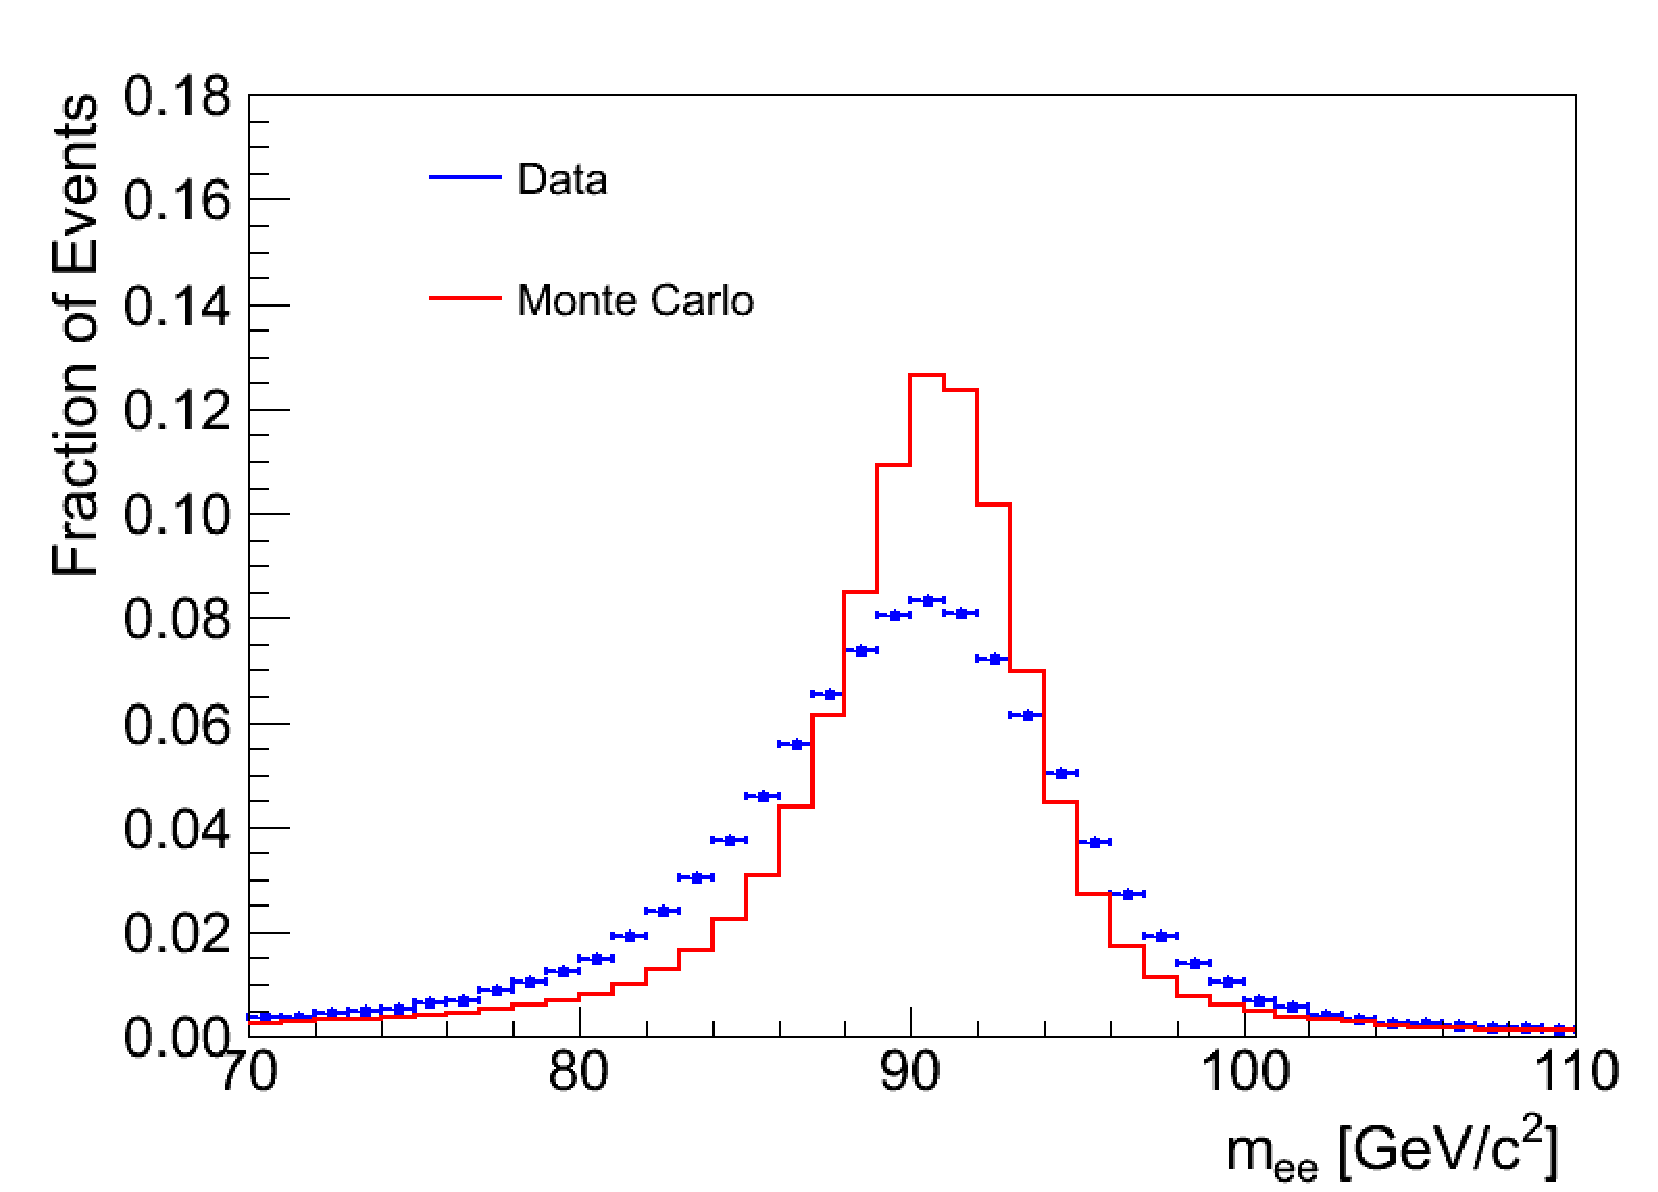
\includegraphics[width=0.45\textwidth]{figures/ZeeMassScaleAndResolutionValidationPlots_EnergyType2_BeforeCorr_CategoryBin5.pdf}
  }
  \caption{Distributions of dielectron mass for events passing \ZToEE\ selection in various kinematic bins of the
  two electrons before performing the energy scale and resolution corrections. The regression including track-related variables
  and without splitting in $p_{T}$ bins is used. ``Central Barrel'' is defined to be the region with
  $|\eta| < 1.0$; ``Outer Barrel'' is defined to be the region with $1.0 \le |\eta| < 1.479$; and ``Endcap''
  is defined to be the region with $1.479 \le |\eta| < 2.5$. } 
  \label{fig:ZMassValidation_BeforeCorr} 
\end{figure}




\begin{figure}[h]
\centering
  \subfigure[Central Barrel, Central Barrel]{
    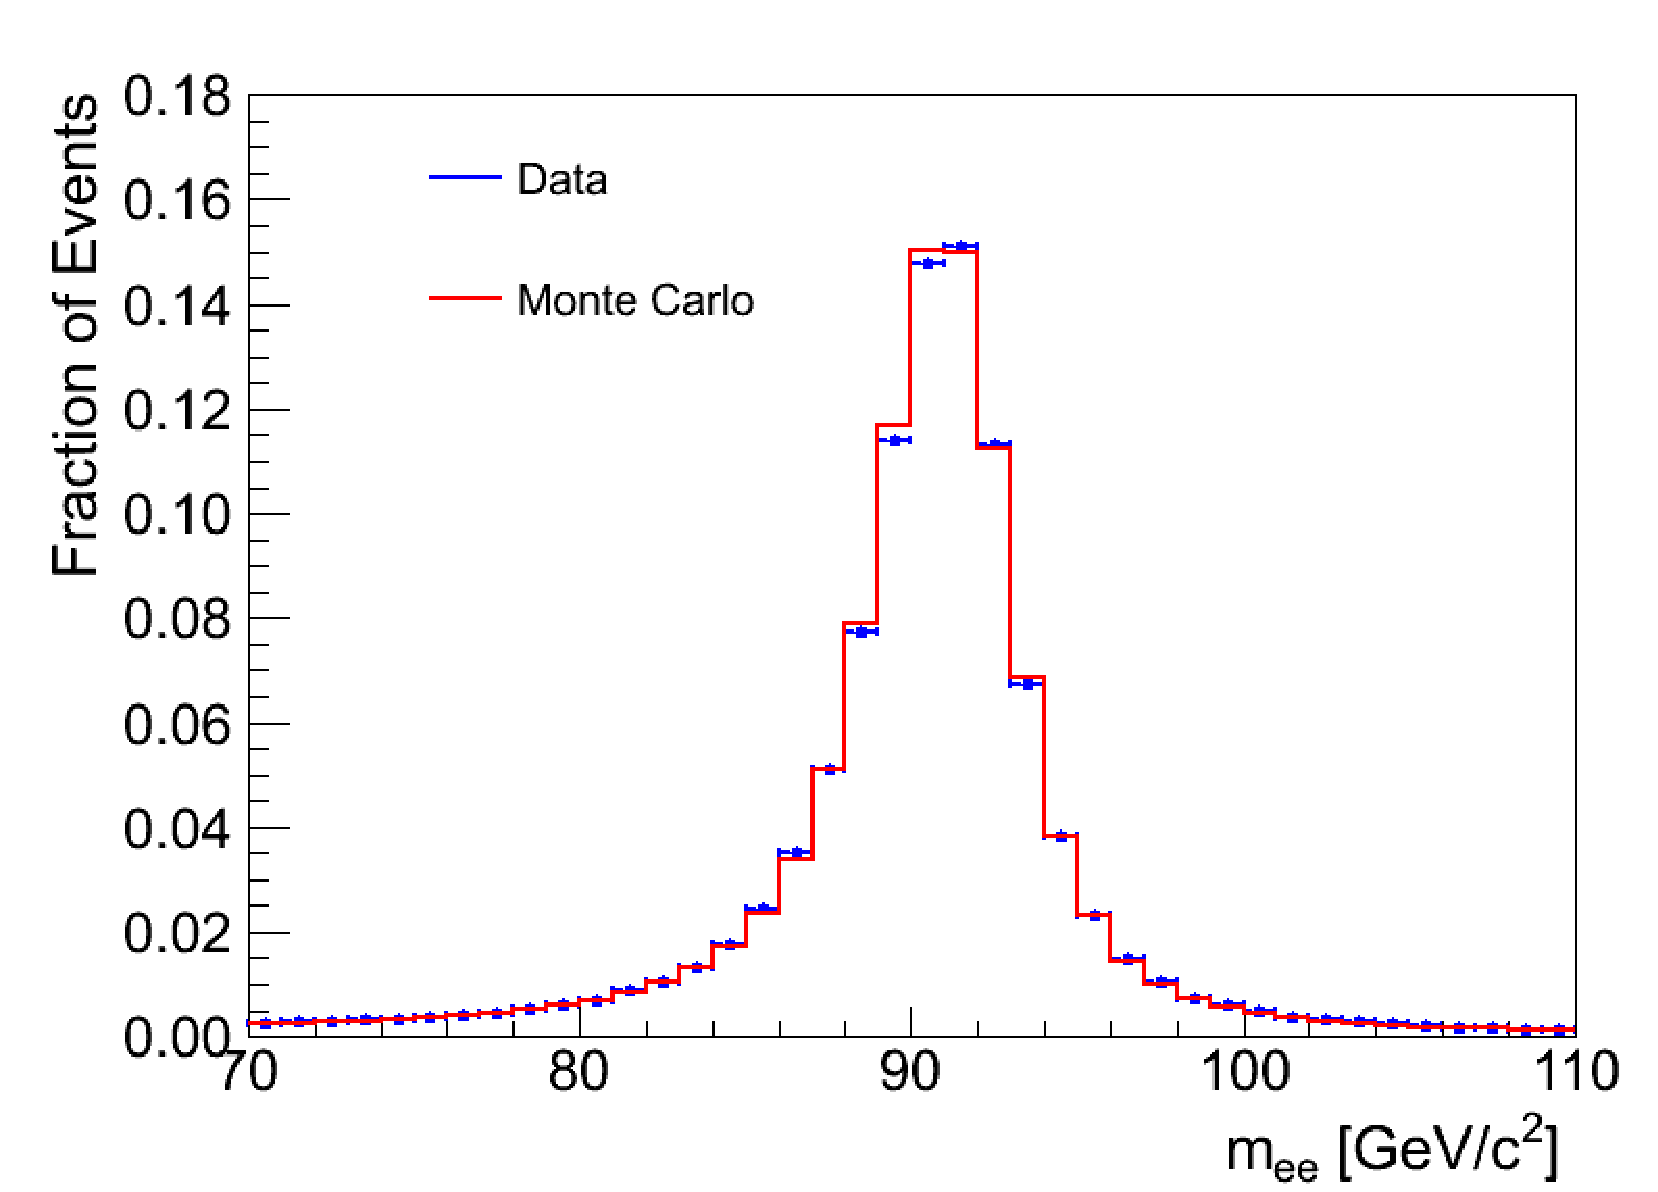
\includegraphics[width=0.45\textwidth]{figures/ZeeMassScaleAndResolutionValidationPlots_EnergyType2_AfterCorr_CategoryBin0.pdf}
  } 
  \subfigure[Central Barrel, Outer Barrel ]{
    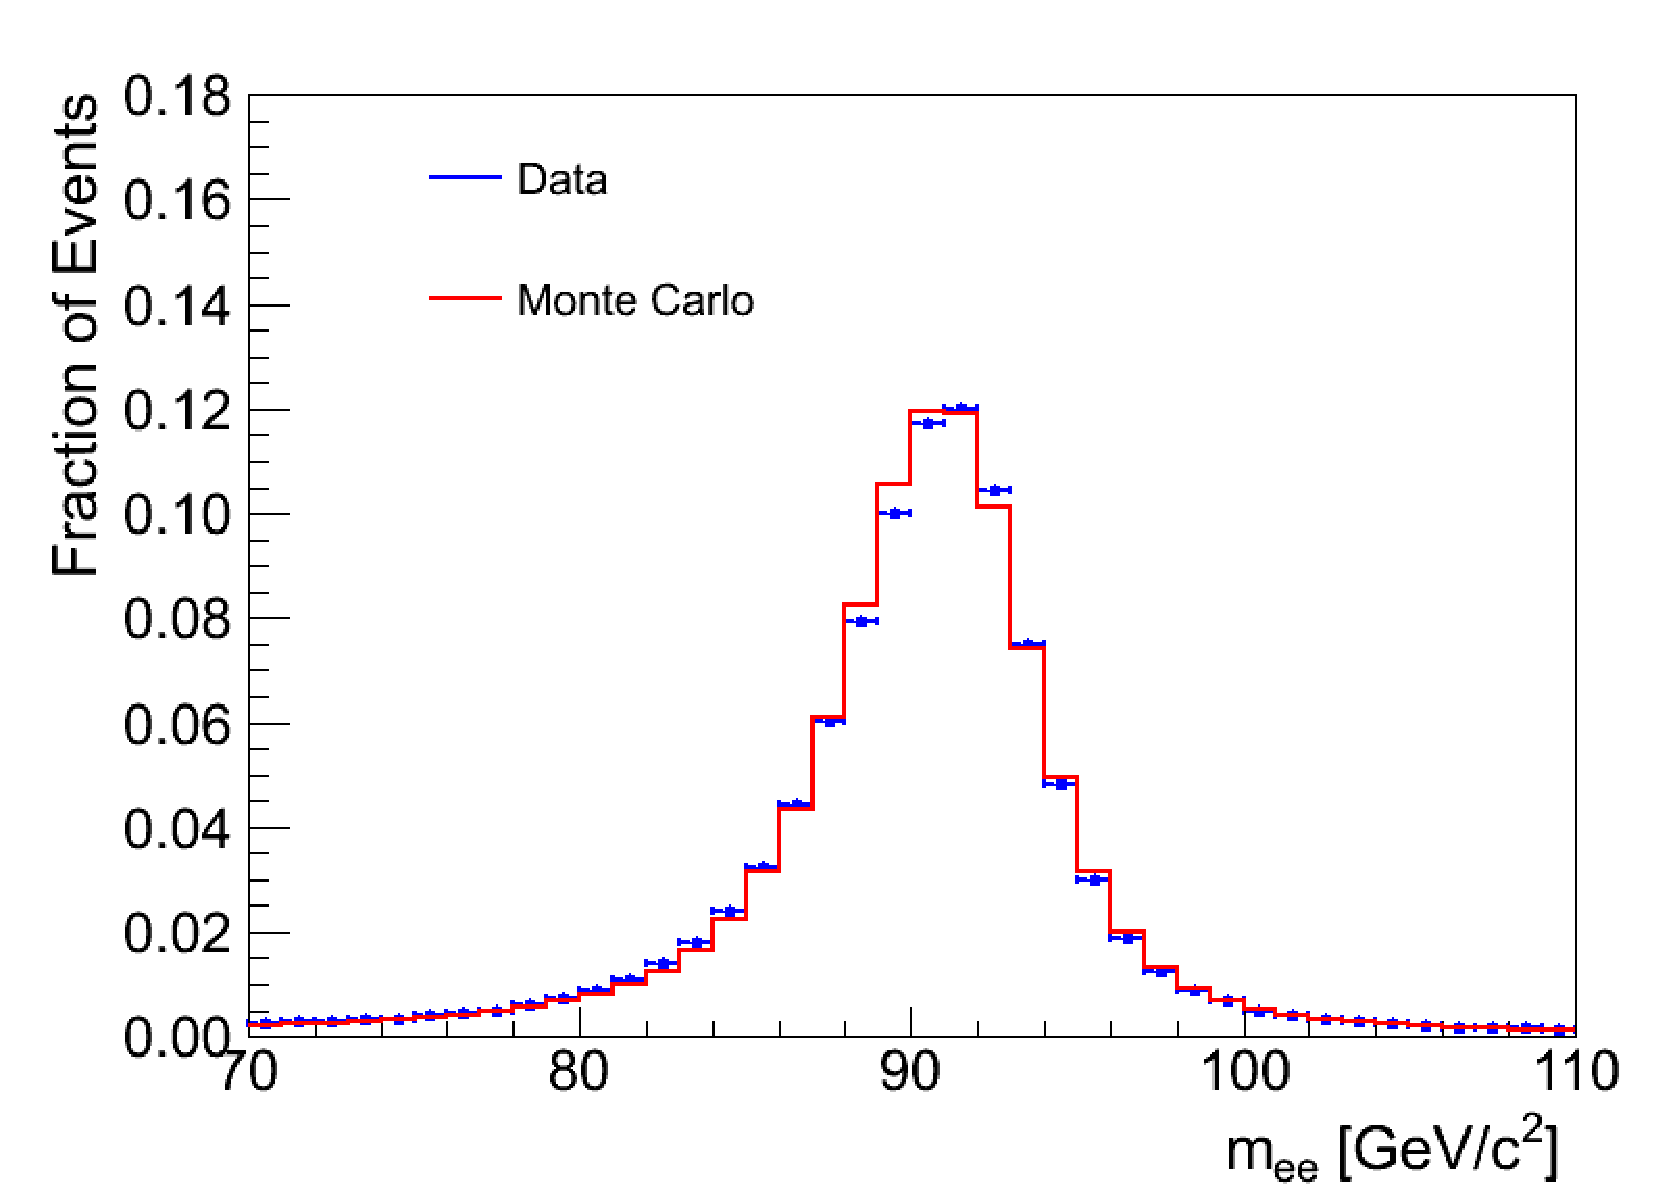
\includegraphics[width=0.45\textwidth]{figures/ZeeMassScaleAndResolutionValidationPlots_EnergyType2_AfterCorr_CategoryBin1.pdf}
  } 
  \subfigure[Central Barrel, Endcap ]{
    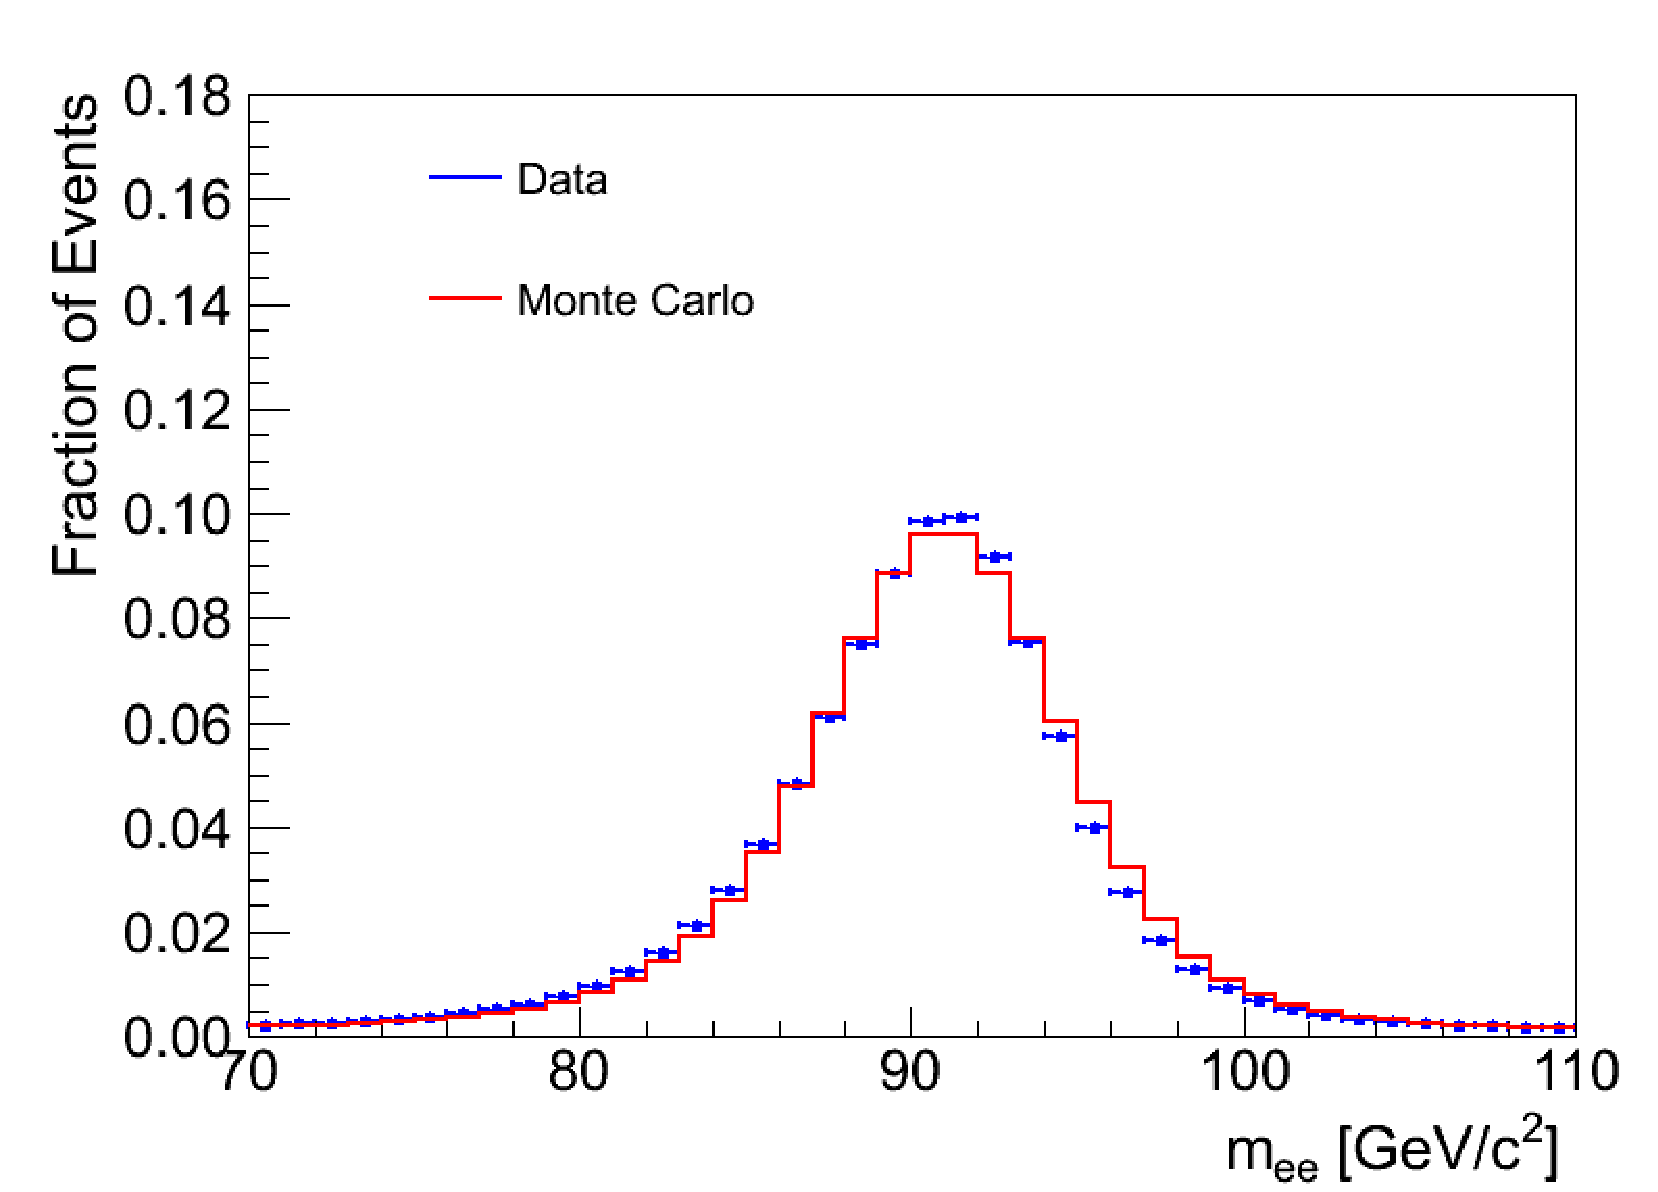
\includegraphics[width=0.45\textwidth]{figures/ZeeMassScaleAndResolutionValidationPlots_EnergyType2_AfterCorr_CategoryBin2.pdf}
  } 
  \subfigure[Outer Barrel, Outer Barrel ]{
    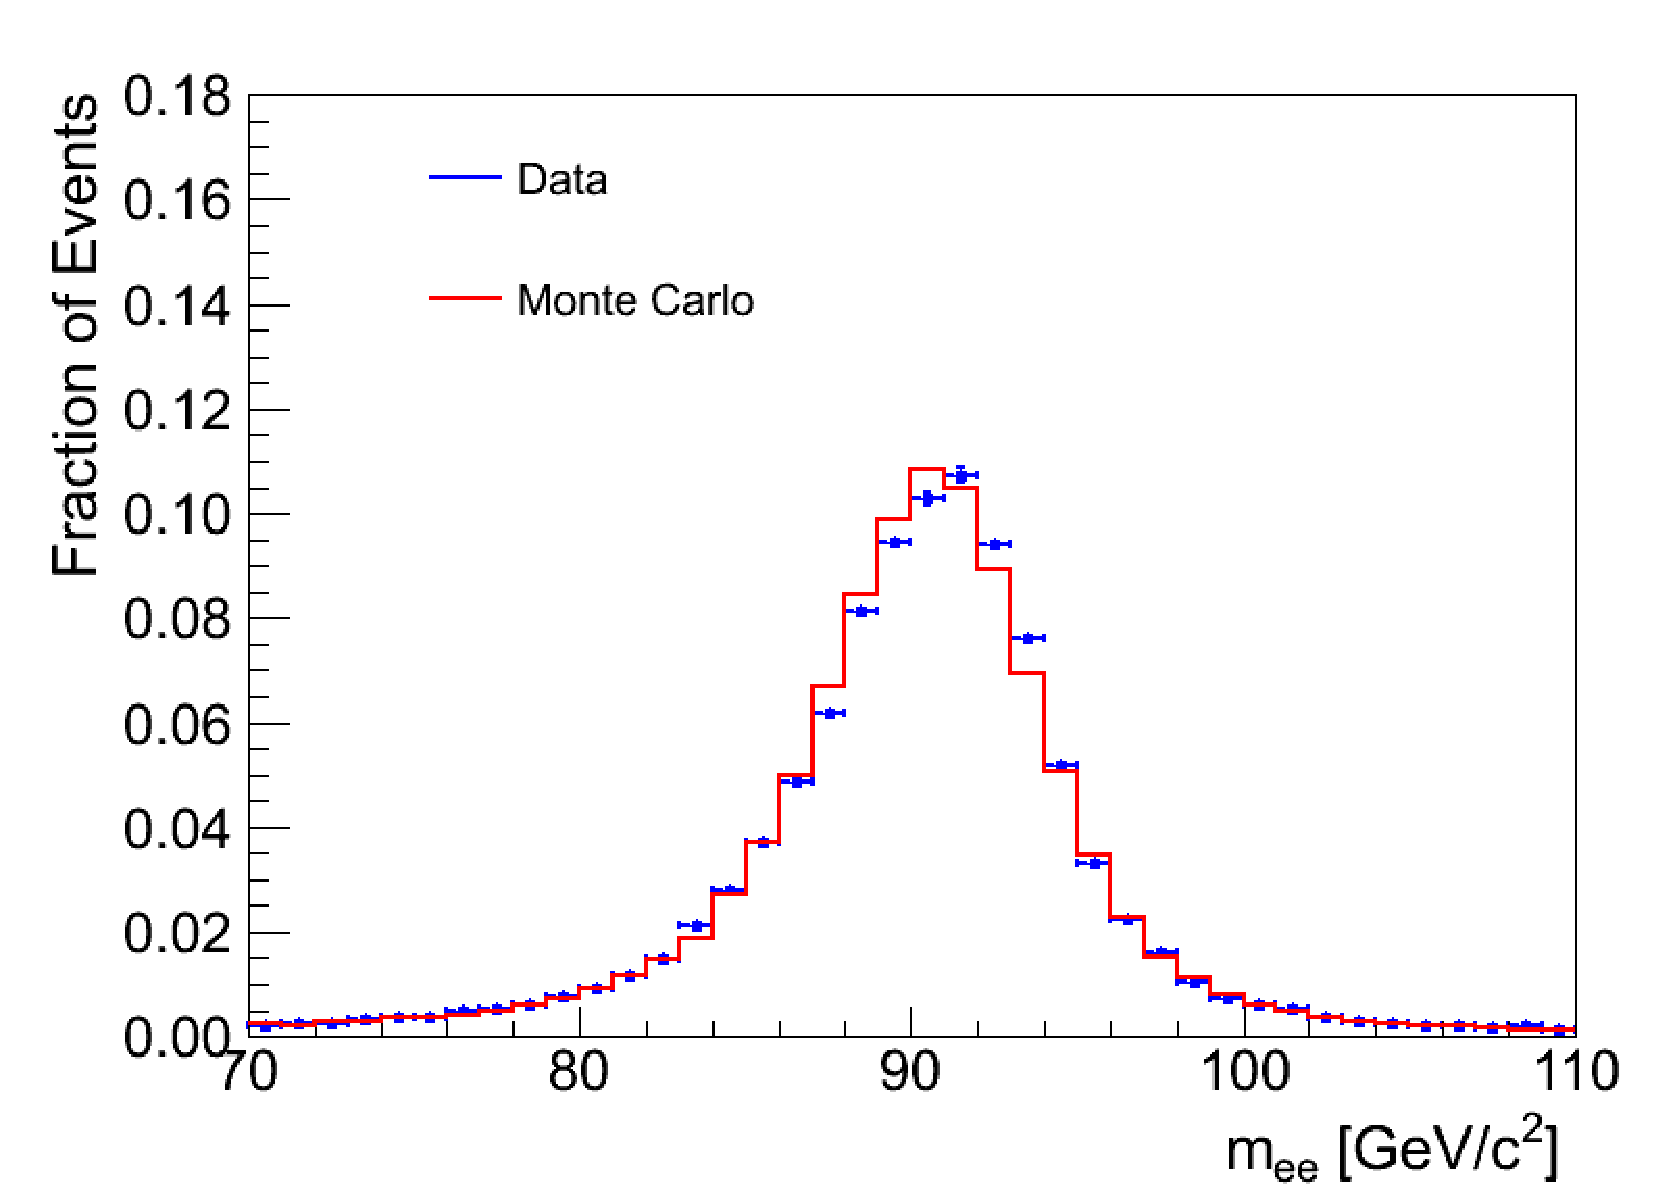
\includegraphics[width=0.45\textwidth]{figures/ZeeMassScaleAndResolutionValidationPlots_EnergyType2_AfterCorr_CategoryBin3.pdf}
  } 
  \subfigure[Outer Barrel, Endcap Barrel]{
    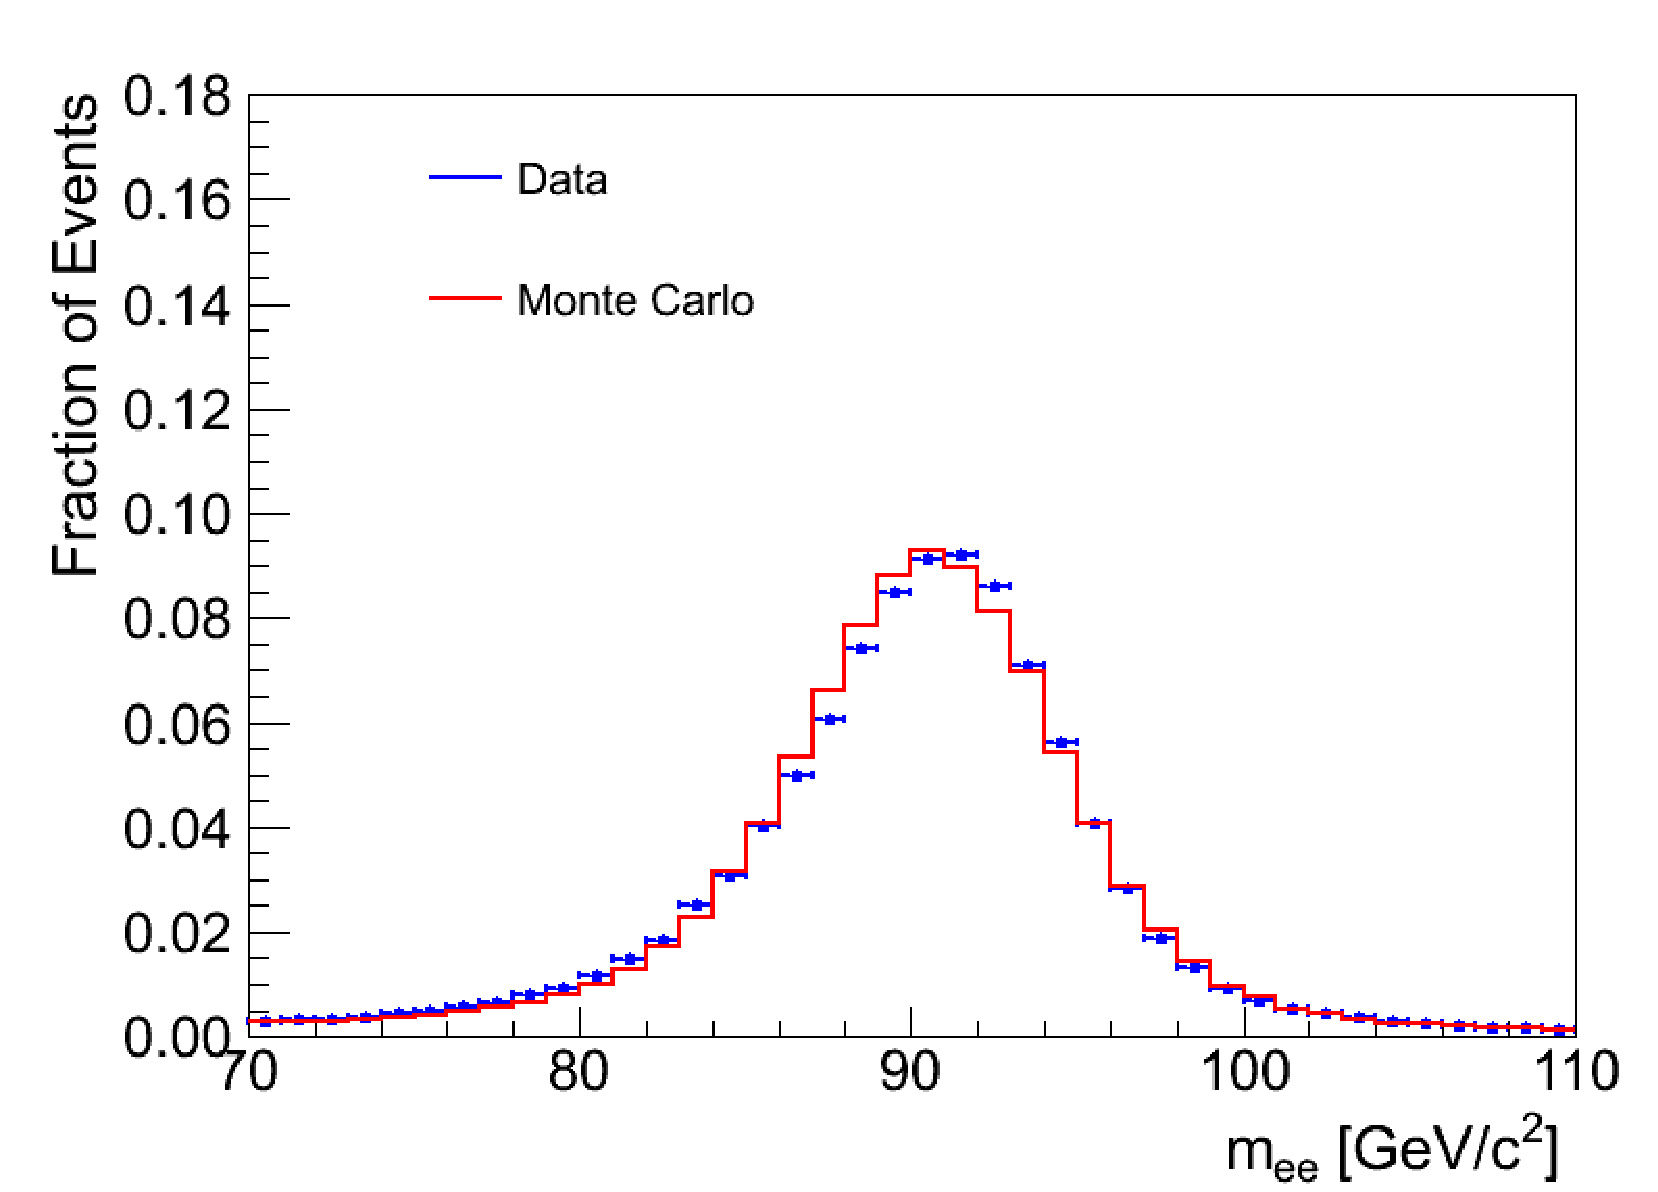
\includegraphics[width=0.45\textwidth]{figures/ZeeMassScaleAndResolutionValidationPlots_EnergyType2_AfterCorr_CategoryBin4.pdf}
  } 
  \subfigure[Endcap Barrel, Endcap Barrel]{
    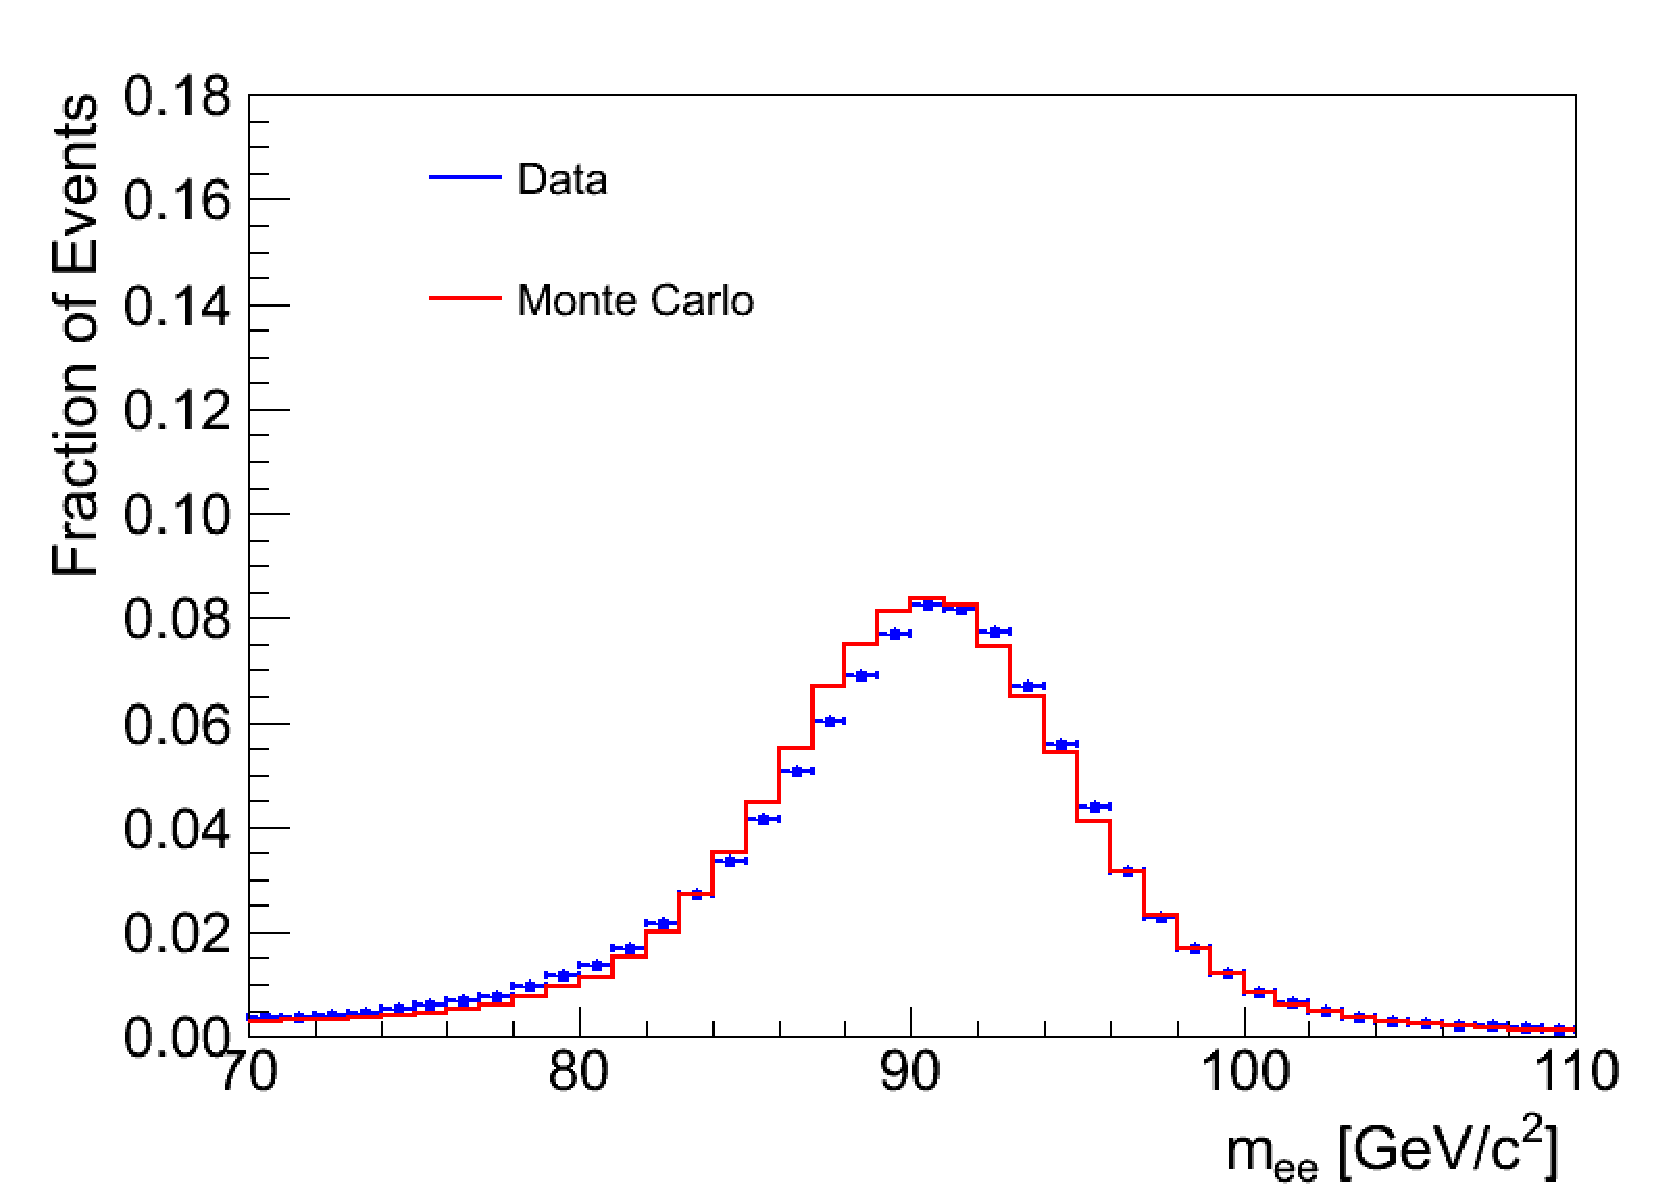
\includegraphics[width=0.45\textwidth]{figures/ZeeMassScaleAndResolutionValidationPlots_EnergyType2_AfterCorr_CategoryBin5.pdf}
  }
  \caption{Distributions of dielectron mass for events passing \ZToEE\ selection in various kinematic bins of the
  two electrons after performing the energy scale and resolution corrections. The regression including track-related variables
  and without splitting in $p_{T}$ bins is used. ``Central Barrel'' is defined to be the region with 
  $|\eta| < 1.0$; ``Outer Barrel'' is defined to be the region with $1.0 \le |\eta| < 1.479$; and ``Endcap''
  is defined to be the region with $1.479 \le |\eta| < 2.5$. } 
  \label{fig:ZMassValidation_AfterCorr} 
\end{figure}


\clearpage

\section{Impact on \HiggsToZZToFourL\ Analysis }

The four different regressions are applied to the \HiggsToZZ\ Monte Carlo simulation sample with mass 
$126$~\GeV\ and the corresponding four lepton mass distributions are compared with the one obtained
using the standard momentum measurement in Figure \ref{fig:HZZMass_Regression_NoCorrection}. 
No additional smearing has been applied yet.
We observe significant improvement in the four lepton mass resolution when using the regression.
 
\begin{figure}[h]
\centering
	\subfigure[4 electron final state]{
		\includegraphics[width=0.45\textwidth]{figures/HZZMass_Regression_4e.pdf}
	} 
	\subfigure[2 electron, 2 muon final state]{
		\includegraphics[width=0.45\textwidth]{figures/HZZMass_Regression_2e2m.pdf}
	} 
	\subfigure[all final states combined]{
		\includegraphics[width=0.6\textwidth]{figures/HZZMass_Regression_all.pdf}
	}
	\caption{Distributions of the reconstructed Higgs boson mass computed using various versions
          of the electron energy regression are compared to the mass distribution obtained using
          the standard electron momentum measurement. }
	\label{fig:HZZMass_Regression_NoCorrection}
\end{figure} 
 

Using the results of Section \ref{sec:DataToMCCorrection}, we perform the appropriate smearing to
each of the different regressions, as well as the standard smearing used for the standard 
momentum measurement \cite{HZZICHEPCMSNote}. The comparison of reconstructed Higgs boson mass distribution
after applying these simulation to data corrections between the standard electron momentum
measurement and the two regressions using track-related variables are shown in 
Figure \ref{fig:HZZMass_Regression_WithCorrection}. The improvement 
in performance using the regression remains after performing these corrections. The performance
is not significantly affected by the splitting of the $p_{T}$ bin, and therefore we choose the
version which does not do the explicit categorization for the sake of simplicity. 
In Figure \ref{fig:HZZMass_CompareFinalstates} we compare the reconstructed Higgs boson
mass distributions between the four electron, two electron two muon, and four muon final states
for the standard electron momentum measurement and the electron regression. We clearly observe
that the regression brings the resolution of the final states involving electrons much closer
to the resolution of the four muon final state. 


\begin{figure}[h]
\centering
	\subfigure[4 electron final state]{
		\includegraphics[width=0.45\textwidth]{figures/HZZMass_RegressionWithCorr_4e.pdf}
	} 
	\subfigure[2 electron, 2 muon final state]{
		\includegraphics[width=0.45\textwidth]{figures/HZZMass_RegressionWithCorr_2e2m.pdf}
	}  
	\subfigure[all final states combined]{
		\includegraphics[width=0.6\textwidth]{figures/HZZMass_RegressionWithCorr_all.pdf}
	}
	\caption{Distributions of the reconstructed Higgs boson mass computed using regressions 
          that include track-related variables are compared to the mass distribution obtained using
          the standard electron momentum measurement. The momentum of individual electrons from the 
          Monte Carlo simulation have been corrected to reflect the resolution measured in data. }
	\label{fig:HZZMass_Regression_WithCorrection}
\end{figure}

\begin{figure}[h]
\centering
	\subfigure[Standard Electron Momentum Measurement]{
		\includegraphics[width=0.45\textwidth]{figures/HZZMassCompareFinalstates_Standard.pdf}
	} 
	\subfigure[Electron Regression]{
		\includegraphics[width=0.45\textwidth]{figures/HZZMassCompareFinalstates_Regression.pdf}
	}  
	\caption{Distributions of the reconstructed Higgs boson mass in different final states are compared
        for the standard electron momentum measurement and the regression. 
        The momentum of individual electrons from the Monte Carlo simulation have been corrected
        to reflect the resolution measured in data. }
	\label{fig:HZZMass_CompareFinalstates}
\end{figure}



\subsection{ Combination with Track Momentum Measurement }

Given that a significant component of the overall improvement brought by the regression technique is
due to the improvement in the ECAL energy measurement, we further study the specific effect of the
inclusion of the tracking measurements into the regression. We define two benchmark regression
reconstruction methods. The electron momentum reconstruction labelled as ``Regression1'' is the combination
of the ECAL energy measured using the regression which does not include any track-related variables, and
the track momentum measurement from the GSF track fit. The standard combination is performed using the
regression estimate of the uncertainty on the ECAl energy measurement \cite{HZZICHEPCMSNote}. The
electron momentum reconstruction labelled as ``Regression2'' is the combined measurement from 
the regression that has been trained with track-related variables included.

In Figure \ref{fig:HZZMassComparison_NoCorr}, we compare the distributions of the reconstructed
Higgs boson mass, before applying any Monte Carlo to data corrections, 
using the default electron momentum reconstruction and the two variations of the
regression reconstruction for the four electron channel, two electron two muon channel, and 
the combination of all channels respectively. We observe relatively small differences in the performance
between the two different regression techniques. The analogous comparison after applying the 
Monte Carlo to data corrections are shown in Figure \ref{fig:HZZMassComparison_WithCorr}.
As the uncertainty of the ECAL regression measurement is increased in the method labelled
``Regression1'', a larger fraction of electrons rely more on the track momentum measurement. As a 
result the resolution becomes visibly worse for the four electron channel. 
 
\begin{figure}[h]
\centering
	\subfigure[4e Channel]{
		\includegraphics[width=0.45\textwidth]{figures/HZZMass_EPCombComparison_RegressionNoCorr_4e.pdf}
	} 
	\subfigure[2e2$\mu$ Channel]{
		\includegraphics[width=0.45\textwidth]{figures/HZZMass_EPCombComparison_RegressionNoCorr_2e2m.pdf}
	}  
	\subfigure[All Channels Combined]{
		\includegraphics[width=0.45\textwidth]{figures/HZZMass_EPCombComparison_RegressionNoCorr_all.pdf}
	}
	\caption{ A comparison of the reconstructed Higgs boson mass distributions before applying any Monte Carlo
          to data corrections for the default electron momentum reconstruction and two different regression reconstructions.
        Regression1 refers to the combination of the regression energy using only ECAL measurements and the
        momentum from the GSF track measurement, and Regression2 refers to the regression measurement that 
        combines ECAL measurements and track measurements.}
	\label{fig:HZZMassComparison_NoCorr}
\end{figure}

\begin{figure}[h]
\centering
	\subfigure[4e Channel]{
		\includegraphics[width=0.45\textwidth]{figures/HZZMass_EPCombComparison_RegressionWithCorr_4e.pdf}
	} 
	\subfigure[2e2$\mu$ Channel]{
		\includegraphics[width=0.45\textwidth]{figures/HZZMass_EPCombComparison_RegressionWithCorr_2e2m.pdf}
	}  
	\subfigure[All Channels Combined]{
		\includegraphics[width=0.45\textwidth]{figures/HZZMass_EPCombComparison_RegressionWithCorr_all.pdf}
	}
	\caption{ A comparison of the reconstructed Higgs boson mass distributions after applying any Monte Carlo
          to data corrections for the default electron momentum reconstruction and two different regression reconstructions.
        Regression1 refers to the combination of the regression energy using only ECAL measurements and the
        momentum from the GSF track measurement, and Regression2 refers to the regression measurement that 
        combines ECAL measurements and track measurements.}
	\label{fig:HZZMassComparison_WithCorr}
\end{figure}

Finally, we perform the signal model fit and extract the $\sigma$ parameter which describes the resolution of
the reconstructed Higgs boson mass. The comparison of the $\sigma$ parameter for the default electron momentum
reconstruction and the two different regression techniques is shown in Table \ref{tab:HiggsResolutionComparison}
for a signal mass of $125~\GeV$. We observe that the ``Regression1'' technique improves the resolution by about
$12\%$ over the standard electron momentum reconstruction 
for both the four electron and two electron two muon channels. The ``Regression2'' technique, which
includes track-related variables in a combined measurement of the electron momentum, gives an improvement
of about $17\%$ for the four electron channel and about $12\%$ for the two electron
two muon channel.

\begin{table}[!ht]
\begin{center} 
\begin{tabular}{|c|c|c|}
\hline
Electron Momentum Type   &   4e Channel               & 2e2$\mu$ Channel    \\  \hline
Default                  &   $3.21~\GeV$              & $2.25~\GeV$         \\  \hline
Regression1              &   $2.81~\GeV$              & $1.97~\GeV$         \\  \hline
Regression2              &   $2.67~\GeV$              & $1.98~\GeV$         \\  \hline
\end{tabular}
\caption{ Comparison of the $\sigma$ parameter describing the resolution of the reconstructed
  Higgs boson mass for different methods for reconstructing the electron momentum.}
\label{tab:HiggsResolutionComparison}
\end{center}
\end{table}




\subsection{Impact on Signal Significance }

We evaluate the impact of the regression on the expected signal significance on a dataset corresponding
to $30~\ifb$. The comparisons of the expected signal significance computed using the representative Asimov Toy
are shown in Figure \ref{fig:SignalSignificance}, and the ratios of expected signal significances are shown
in Figure \ref{fig:SignalSignificanceRatio}. We observe an improvement to the signal significance of 
about $7\%$ for the four electron final state, $5\%$ for the two electron two muon final state,
and $3\%$ for the combined analysis.


\begin{figure}[h]
\centering
	\subfigure[4e Channel]{
		\includegraphics[width=0.45\textwidth]{figures/expsignif_4e.pdf}
	} 
	\subfigure[2e2$\mu$ Channel]{
		\includegraphics[width=0.45\textwidth]{figures/expsignif_2e2mu.pdf}
	}  
	\subfigure[All Channels Combined]{
		\includegraphics[width=0.45\textwidth]{figures/expsignif_allchannels.pdf}
	}
	\caption{ A comparison of the expected signal significance at $30\ifb$ are shown for
        the default electron momentum reconstruction and two different regression reconstructions.
        Regression1 refers to the combination of the regression energy using only ECAL measurements and the
        momentum from the GSF track measurement, and Regression2 refers to the regression measurement that 
        combines ECAL measurements and track measurements.}
	\label{fig:SignalSignificance}
\end{figure}

\begin{figure}[h]
\centering
	\subfigure[4e Channel]{
		\includegraphics[width=0.45\textwidth]{figures/expsignif_ratio_4e.pdf}
	} 
	\subfigure[2e2$\mu$ Channel]{
		\includegraphics[width=0.45\textwidth]{figures/expsignif_ratio_2e2mu.pdf}
	}  
	\subfigure[All Channels Combined]{
		\includegraphics[width=0.45\textwidth]{figures/expsignif_ratio_allchannels.pdf}
	}
	\caption{ Ratios of the expected signal significance using the regression electron energy measurements
          to the expected signal significance using the default electron momentum reconstruction at $30\ifb$ are shown.}
	\label{fig:SignalSignificanceRatio}
\end{figure}


\subsection{Impact on Mass Measurement }

The impact of the electron energy regression on the Higgs boson mass measurement are 
summarized in Tables \ref{tab:MassMeasurementUncertainty_4e}, \ref{tab:MassMeasurementUncertainty_2e2mu},
and \ref {tab:MassMeasurementUncertainty_combined}, where the uncertainties estimated
using the asimov toy dataset for $30~\ifb$ are compared using the default electron momentum
reconstruction and the electron momentum reconstruction using the regression. We observe reductions
in the uncertainty of the mass measurement of about $20\%$ for the four electron channel only,
$11\%$ for the two electron two muon channel only, and $5\%$ for the combined measurement.

\begin{table}[!ht]
\begin{center} 
\begin{tabular}{|c|c|c|c|}
\hline
Electron Momentum Type   &   Statistical Uncertainty & Systematic Uncertainty  & Total Uncertainty    \\  \hline
Default                  &   $2.93~\GeV$              & $1.43~\GeV$              & $3.26~\GeV$        \\  \hline
Regression1              &   $2.57~\GeV$              & $1.16~\GeV$              & $2.82~\GeV$        \\  \hline
Regression2              &   $2.39~\GeV$              & $1.05~\GeV$              & $2.61~\GeV$        \\  \hline
\end{tabular}
\caption{ Uncertainties in the Higgs boson mass measurement performed using the four electron channel only
are compared between different methods for reconstructing the electron momentum.}
\label{tab:MassMeasurementUncertainty_4e}
\end{center}
\end{table}

\begin{table}[!ht]
\begin{center} 
\begin{tabular}{|c|c|c|c|}
\hline
Electron Momentum Type   &   Statistical Uncertainty & Systematic Uncertainty  & Total Uncertainty    \\  \hline
Default                  &   $1.09~\GeV$              & $0.60~\GeV$              & $1.24~\GeV$        \\  \hline
Regression1              &   $0.96~\GeV$              & $0.59~\GeV$              & $1.13~\GeV$        \\  \hline
Regression2              &   $0.94~\GeV$              & $0.59~\GeV$              & $1.11~\GeV$        \\  \hline
\end{tabular}
\caption{ Uncertainties in the Higgs boson mass measurement performed using the two electron two muon channel only
are compared between different methods for reconstructing the electron momentum.}
\label{tab:MassMeasurementUncertainty_2e2mu}
\end{center}
\end{table}

\begin{table}[!ht]
\begin{center} 
\begin{tabular}{|c|c|c|c|}
\hline
Electron Momentum Type   &   Statistical Uncertainty & Systematic Uncertainty  & Total Uncertainty    \\  \hline
Default                  &   $0.53~\GeV$              & $0.41~\GeV$              & $0.67~\GeV$        \\  \hline
Regression1              &   $0.51~\GeV$              & $0.39~\GeV$              & $0.64~\GeV$        \\  \hline
Regression2              &   $0.51~\GeV$              & $0.39~\GeV$              & $0.64~\GeV$        \\  \hline
\end{tabular}
\caption{ Uncertainties in the Higgs boson mass measurement performed using all channels
are compared between different methods for reconstructing the electron momentum.}
\label{tab:MassMeasurementUncertainty_combined}
\end{center}
\end{table}



\section{Conclusion}

We described the training and performance evaluation of a multivariate regression 
approach to measuring the momentum of electrons. The regression method is applied
to the \HiggsToZZ\ analysis where we observe an improvement of $17\%$ for the
four electron channel and $12\%$ for the two electron two muon channel. Propagating
this improvement in resolution to the signal extraction results in an improvement
of the expected signal significance at $30~\ifb$ of about $7\%$ for the four electron
channel, $5\%$ for the two electron two muon channel, and $3\%$ for the
combined analysis. Propagating this improvement in resolution to the Higgs boson
mass measurement in the four lepton channel gives a reduction in the 
mass uncertainty of about $20\%$ in the four electron channel, $11\%$ 
in the two electron two muon channel, and $5\%$ for the combination
of all channels.


%===================================================================================================
\clearpage

\vspace*{-0.2cm}
\thebibliography{12}

\bibitem{Item1}
 

%===================================================================================================

\appendix
\appendixpage

\section{Energy Scale and Resolution Fits}
\label{sec:ScaleAndResolutionFits}
\subsection{Standard Electron Momentum Measurement }

\begin{figure}[h]
\centering
	\subfigure[$0.0 \le |\eta| < 1.0$]{
		\includegraphics[width=0.45\textwidth]{figures/ZMassFits/ZeeFits_MC_EnergyType0_CategoryBin0.pdf}
	} 
	\subfigure[$1.0 \le |\eta| < 1.479$]{
		\includegraphics[width=0.45\textwidth]{figures/ZMassFits/ZeeFits_MC_EnergyType0_CategoryBin1.pdf}
	}  
	\subfigure[$1.479 \le |\eta| < 2.5$]{
		\includegraphics[width=0.45\textwidth]{figures/ZMassFits/ZeeFits_MC_EnergyType0_CategoryBin2.pdf}
	}
	\caption{Fits of the dielectron mass distribution in the Monte Carlo simulation to
        a Breit-Wigner convoluted with a Crystal Ball resolution function. The fitted parameters 
        of the Crystal Ball function are shown. The standard electron momentum measurement is 
        used.}
	\label{fig:ZMassFit_MC_Standard}
\end{figure}

\begin{figure}[h]
\centering
	\subfigure[$0.0 \le |\eta| < 1.0$]{
		\includegraphics[width=0.45\textwidth]{figures/ZMassFits/ZeeFits_2012Data_EnergyType0_CategoryBin0.pdf}
	} 
	\subfigure[$1.0 \le |\eta| < 1.479$]{
		\includegraphics[width=0.45\textwidth]{figures/ZMassFits/ZeeFits_2012Data_EnergyType0_CategoryBin1.pdf}
	}  
	\subfigure[$1.479 \le |\eta| < 2.5$]{
		\includegraphics[width=0.45\textwidth]{figures/ZMassFits/ZeeFits_2012Data_EnergyType0_CategoryBin2.pdf}
	}
	\caption{Fits of the dielectron mass distribution in the 2012 data to
        a Breit-Wigner convoluted with a Crystal Ball resolution function. The parameters $a_{\mathrm{CB}}$ 
        and $n_{\mathrm{CB}}$ describing the low side tail of the Crystal Ball function have been fixed to the values
        obtained from the corresponding fit to the MC simulation. The mass shift and width parameters 
        of the Crystal Ball function are shown. The standard electron momentum measurement is 
        used.}
	\label{fig:ZMassFit_2012Data_Standard}
\end{figure}
 
\clearpage

\subsection{Regression Without Track-related Variables and Without split $p_{T}$ bins }

\begin{figure}[h]
\centering
	\subfigure[$0.0 \le |\eta| < 1.0$]{
		\includegraphics[width=0.45\textwidth]{figures/ZMassFits/ZeeFits_MC_EnergyType1_CategoryBin0.pdf}
	} 
	\subfigure[$1.0 \le |\eta| < 1.479$]{
		\includegraphics[width=0.45\textwidth]{figures/ZMassFits/ZeeFits_MC_EnergyType1_CategoryBin1.pdf}
	}  
	\subfigure[$1.479 \le |\eta| < 2.5$]{
		\includegraphics[width=0.45\textwidth]{figures/ZMassFits/ZeeFits_MC_EnergyType1_CategoryBin2.pdf}
	}
	\caption{Fits of the dielectron mass distribution in the Monte Carlo simulation to
        a Breit-Wigner convoluted with a Crystal Ball resolution function. The fitted parameters 
        of the Crystal Ball function are shown. The regression trained without track-related variables
        and without $p_{T}$ bin splitting has been used to compute the electron momentum.}
	\label{fig:ZMassFit_MC_Regression1}
\end{figure}

\begin{figure}[h]
\centering
	\subfigure[$0.0 \le |\eta| < 1.0$]{
		\includegraphics[width=0.45\textwidth]{figures/ZMassFits/ZeeFits_2012Data_EnergyType1_CategoryBin0.pdf}
	} 
	\subfigure[$1.0 \le |\eta| < 1.479$]{
		\includegraphics[width=0.45\textwidth]{figures/ZMassFits/ZeeFits_2012Data_EnergyType1_CategoryBin1.pdf}
	}  
	\subfigure[$1.479 \le |\eta| < 2.5$]{
		\includegraphics[width=0.45\textwidth]{figures/ZMassFits/ZeeFits_2012Data_EnergyType1_CategoryBin2.pdf}
	}
	\caption{Fits of the dielectron mass distribution in the 2012 data to
        a Breit-Wigner convoluted with a Crystal Ball resolution function. The parameters $a_{\mathrm{CB}}$ 
        and $n_{\mathrm{CB}}$ describing the low side tail of the Crystal Ball function have been fixed to the values
        obtained from the corresponding fit to the MC simulation. The mass shift and width parameters 
        of the Crystal Ball function are shown. The regression trained without track-related variables
        and without $p_{T}$ bin splitting has been used to compute the electron momentum.}
	\label{fig:ZMassFit_2012Data_Regression1}
\end{figure}

\clearpage


\subsection{Regression Without Track-related Variables and With split $p_{T}$ bins }

\begin{figure}[h]
\centering
	\subfigure[$0.0 \le |\eta| < 1.0$]{
		\includegraphics[width=0.45\textwidth]{figures/ZMassFits/ZeeFits_MC_EnergyType2_CategoryBin0.pdf}
	} 
	\subfigure[$1.0 \le |\eta| < 1.479$]{
		\includegraphics[width=0.45\textwidth]{figures/ZMassFits/ZeeFits_MC_EnergyType2_CategoryBin1.pdf}
	}  
	\subfigure[$1.479 \le |\eta| < 2.5$]{
		\includegraphics[width=0.45\textwidth]{figures/ZMassFits/ZeeFits_MC_EnergyType2_CategoryBin2.pdf}
	}
	\caption{Fits of the dielectron mass distribution in the Monte Carlo simulation to
        a Breit-Wigner convoluted with a Crystal Ball resolution function. The fitted parameters 
        of the Crystal Ball function are shown. The regression trained with track-related variables
        and without $p_{T}$ bin splitting has been used to compute the electron momentum.}
	\label{fig:ZMassFit_MC_Regression2}
\end{figure}

\begin{figure}[h]
\centering
	\subfigure[$0.0 \le |\eta| < 1.0$]{
		\includegraphics[width=0.45\textwidth]{figures/ZMassFits/ZeeFits_2012Data_EnergyType2_CategoryBin0.pdf}
	} 
	\subfigure[$1.0 \le |\eta| < 1.479$]{
		\includegraphics[width=0.45\textwidth]{figures/ZMassFits/ZeeFits_2012Data_EnergyType2_CategoryBin1.pdf}
	}  
	\subfigure[$1.479 \le |\eta| < 2.5$]{
		\includegraphics[width=0.45\textwidth]{figures/ZMassFits/ZeeFits_2012Data_EnergyType2_CategoryBin2.pdf}
	}
	\caption{Fits of the dielectron mass distribution in the 2012 data to
        a Breit-Wigner convoluted with a Crystal Ball resolution function. The parameters $a_{\mathrm{CB}}$ 
        and $n_{\mathrm{CB}}$ describing the low side tail of the Crystal Ball function have been fixed to the values
        obtained from the corresponding fit to the MC simulation. The mass shift and width parameters 
        of the Crystal Ball function are shown. The regression trained with track-related variables
        and without $p_{T}$ bin splitting has been used to compute the electron momentum.}
	\label{fig:ZMassFit_2012Data_Regression2}
\end{figure}

\clearpage

\subsection{Regression With Track-related Variables and Without split $p_{T}$ bins }

\begin{figure}[h]
\centering
	\subfigure[$0.0 \le |\eta| < 1.0$]{
		\includegraphics[width=0.45\textwidth]{figures/ZMassFits/ZeeFits_MC_EnergyType3_CategoryBin0.pdf}
	} 
	\subfigure[$1.0 \le |\eta| < 1.479$]{
		\includegraphics[width=0.45\textwidth]{figures/ZMassFits/ZeeFits_MC_EnergyType3_CategoryBin1.pdf}
	}  
	\subfigure[$1.479 \le |\eta| < 2.5$]{
		\includegraphics[width=0.45\textwidth]{figures/ZMassFits/ZeeFits_MC_EnergyType3_CategoryBin2.pdf}
	}
	\caption{Fits of the dielectron mass distribution in the Monte Carlo simulation to
        a Breit-Wigner convoluted with a Crystal Ball resolution function. The fitted parameters 
        of the Crystal Ball function are shown. The regression trained without track-related variables
        and with $p_{T}$ bin splitting has been used to compute the electron momentum.}
	\label{fig:ZMassFit_MC_Regression3}
\end{figure}

\begin{figure}[h]
\centering
	\subfigure[$0.0 \le |\eta| < 1.0$]{
		\includegraphics[width=0.45\textwidth]{figures/ZMassFits/ZeeFits_2012Data_EnergyType3_CategoryBin0.pdf}
	} 
	\subfigure[$1.0 \le |\eta| < 1.479$]{
		\includegraphics[width=0.45\textwidth]{figures/ZMassFits/ZeeFits_2012Data_EnergyType3_CategoryBin1.pdf}
	}  
	\subfigure[$1.479 \le |\eta| < 2.5$]{
		\includegraphics[width=0.45\textwidth]{figures/ZMassFits/ZeeFits_2012Data_EnergyType3_CategoryBin2.pdf}
	}
	\caption{Fits of the dielectron mass distribution in the 2012 data to
        a Breit-Wigner convoluted with a Crystal Ball resolution function. The parameters $a_{\mathrm{CB}}$ 
        and $n_{\mathrm{CB}}$ describing the low side tail of the Crystal Ball function have been fixed to the values
        obtained from the corresponding fit to the MC simulation. The mass shift and width parameters 
        of the Crystal Ball function are shown. The regression trained without track-related variables
        and with $p_{T}$ bin splitting has been used to compute the electron momentum.}
	\label{fig:ZMassFit_2012Data_Regression3}
\end{figure}

\clearpage

\subsection{Regression With Track-related Variables and With split $p_{T}$ bins }

\begin{figure}[h]
\centering
	\subfigure[$0.0 \le |\eta| < 1.0$]{
		\includegraphics[width=0.45\textwidth]{figures/ZMassFits/ZeeFits_MC_EnergyType4_CategoryBin0.pdf}
	} 
	\subfigure[$1.0 \le |\eta| < 1.479$]{
		\includegraphics[width=0.45\textwidth]{figures/ZMassFits/ZeeFits_MC_EnergyType4_CategoryBin1.pdf}
	}  
	\subfigure[$1.479 \le |\eta| < 2.5$]{
		\includegraphics[width=0.45\textwidth]{figures/ZMassFits/ZeeFits_MC_EnergyType4_CategoryBin2.pdf}
	}
	\caption{Fits of the dielectron mass distribution in the Monte Carlo simulation to
        a Breit-Wigner convoluted with a Crystal Ball resolution function. The fitted parameters 
        of the Crystal Ball function are shown. The regression trained with track-related variables
        and with $p_{T}$ bin splitting has been used to compute the electron momentum.}
	\label{fig:ZMassFit_MC_Regression4}
\end{figure}

\begin{figure}[h]
\centering
	\subfigure[$0.0 \le |\eta| < 1.0$]{
		\includegraphics[width=0.45\textwidth]{figures/ZMassFits/ZeeFits_2012Data_EnergyType4_CategoryBin0.pdf}
	} 
	\subfigure[$1.0 \le |\eta| < 1.479$]{
		\includegraphics[width=0.45\textwidth]{figures/ZMassFits/ZeeFits_2012Data_EnergyType4_CategoryBin1.pdf}
	}  
	\subfigure[$1.479 \le |\eta| < 2.5$]{
		\includegraphics[width=0.45\textwidth]{figures/ZMassFits/ZeeFits_2012Data_EnergyType4_CategoryBin2.pdf}
	}
	\caption{Fits of the dielectron mass distribution in the 2012 data to
        a Breit-Wigner convoluted with a Crystal Ball resolution function. The parameters $a_{\mathrm{CB}}$ 
        and $n_{\mathrm{CB}}$ describing the low side tail of the Crystal Ball function have been fixed to the values
        obtained from the corresponding fit to the MC simulation. The mass shift and width parameters 
        of the Crystal Ball function are shown. The regression trained with track-related variables
        and with $p_{T}$ bin splitting has been used to compute the electron momentum.}
	\label{fig:ZMassFit_2012Data_Regression4}
\end{figure}

\clearpage


\end{document}
